% Arquivo LaTeX de exemplo de dissertação/tese a ser apresentada à CPG do IME-USP
%
% Criação: Jesús P. Mena-Chalco
% Revisão: Fabio Kon e Paulo Feofiloff
% Adaptação para UTF8, biblatex e outras melhorias: Nelson Lago
%
% Except where otherwise indicated, these files are distributed under
% the MIT Licence. The example text, which includes the tutorial and
% examples as well as the explanatory comments in the source, are
% available under the Creative Commons Attribution International
% Licence, v4.0 (CC-BY 4.0) - https://creativecommons.org/licenses/by/4.0/


%%%%%%%%%%%%%%%%%%%%%%%%%%%%%%%%%%%%%%%%%%%%%%%%%%%%%%%%%%%%%%%%%%%%%%%%%%%%%%%%
%%%%%%%%%%%%%%%%%%%%%%%%%%%%%%% PREÂMBULO LaTeX %%%%%%%%%%%%%%%%%%%%%%%%%%%%%%%%
%%%%%%%%%%%%%%%%%%%%%%%%%%%%%%%%%%%%%%%%%%%%%%%%%%%%%%%%%%%%%%%%%%%%%%%%%%%%%%%%

% "Book" tem capítulos (e partes, mas normalmente não usamos) e, se o documento
% é frente-e-verso, cada capítulo começa em uma página de numeração ímpar.
% Report é similar, mas cada capítulo começa em uma nova página, par ou ímpar.
% É possível mudar esse comportamento com a opção "openany". Observe que você
% pode adaptar este modelo para escrever artigos, mudando a classe do
% documento de "book" para "article" ou a classe de algum periódico específico.
% No entanto, o arquivo "artigo.tex" é um ponto de partida melhor: ele é
% similar a este, mas já inclui as mudanças necessárias para a classe article.
%
% A opção frente-e-verso aqui significa, por exemplo, que as margens das páginas
% ímpares e pares são diferentes ou que números de página aparecem à direita
% ou à esquerda alternadamente. Nada impede que você crie um documento "só
% frente" e, ao imprimir, faça a impressão frente-e-verso.
%
% Aqui também definimos a língua padrão do documento e línguas adicionais. A
% classe em si não usa essa informação mas, passando as opções de língua aqui,
% elas são repassadas para todas as packages, e diversas packages mudam
% seu comportamento em função da língua (em especial, babel/polyglossia).
% A última língua da lista é a língua padrão do documento.
\documentclass[12pt,twoside,brazil,english]{book}
%\documentclass[12pt,twoside,english,brazil]{book}

% Com papel tamanho A4, queremos estas margens:
%
% topo: 32mm
% pé: 28mm
% esquerda/interna: 24mm
% direita/externa: 34mm
%
% Para isso, definimos os tamanhos do texto, do cabeçalho e do rodapé,
% e deixamos a package geometry calcular os demais valores. Assim,
% obtemos o mesmo resultado impresso, mas com margens diferentes, se
% o tamanho do papel for diferente.

\usepackage[a4paper]{geometry}

\geometry{
  %top=32mm,
  %bottom=28mm,
  %left=24mm,
  %right=34mm,
  textwidth=152mm, % 210-24-34
  textheight=237mm, % 297-32-28
  vmarginratio=8:7, % 32:28
  hmarginratio=12:17, % 24:34
  % Com geometry, esta medida não é tão relevante; basta garantir que ela
  % seja menor que "top" e que o texto do cabeçalho caiba nela.
  headheight=25.4mm,
  % distância entre o início do texto principal e a base do cabeçalho;
  % ou seja, o cabeçalho "invade" a margem superior nessa medida. Essa
  % é a medida que determina a posição do cabeçalho
  headsep=11mm,
  footskip=10mm,
  marginpar=20mm,
  marginparsep=5mm,
}

% Vários pacotes e opções de configuração genéricos; para personalizar o
% resultado, modifique estes arquivos.
%%%%%%%%%%%%%%%%%%%%%%%%%%%%%%%%%%%%%%%%%%%%%%%%%%%%%%%%%%%%%%%%%%%%%%%%%%%%%%%%
%%%%%%%%%%%%%%%%%%%%%%% CONFIGURAÇÕES E PACOTES BÁSICOS %%%%%%%%%%%%%%%%%%%%%%%%
%%%%%%%%%%%%%%%%%%%%%%%%%%%%%%%%%%%%%%%%%%%%%%%%%%%%%%%%%%%%%%%%%%%%%%%%%%%%%%%%

% Vários comandos auxiliares para o desenvolvimento de packages e classes;
% aqui, usamos em alguns comandos de formatação e condicionais.
\usepackage{etoolbox}
\usepackage{xstring}
\usepackage{xparse}
\usepackage{regexpatch}
% Estas não estão em uso mas podem ser úteis.
%\usepackage{ltxcmds}
%\usepackage{letltxmacro}

% Esta package permite detectar XeTeX, LuaTeX e pdfTeX, mas pode não estar
% disponível em todas as instalações de TeX.
%\usepackage{iftex}
% Por conta disso, usaremos estas (que não detectam pdfTeX):
\usepackage{ifxetex}
\usepackage{ifluatex}

\newbool{unicodeengine}
\ifboolexpr{bool{xetex} or bool{luatex}}
  {\booltrue{unicodeengine}}
  {\boolfalse{unicodeengine}}

% Detecta se estamos produzindo um arquivo PDF ou DVI (lembrando que tanto
% pdfTeX quanto LuaTeX podem gerar ambos)
\usepackage{ifpdf}

% Algumas packages "padrão" da AMS, que são praticamente  obrigatórias.
% Algumas delas devem ser carregadas antes de unicode-math ou das
% definições das fontes do documento.
\usepackage{amssymb}
\usepackage{amsthm}
\usepackage{amsmath}
\usepackage{mathtools}

\ifunicodeengine
  % Não é preciso carregar fontenc e inputenc com LuaTeX e XeTeX!
  \usepackage{fontspec}
  \usepackage{unicode-math}
\else
  % "fontenc" é um parâmetro interno do LaTeX. Com pdfLaTeX, o fontenc
  % default é OT1, mas ele tem algumas limitações; a mais importante é
  % que, com ele, palavras acentuadas não podem ser hifenizadas. Por
  % conta disso, quase todos os documentos LaTeX utilizam o fontenc T1.
  % A escolha do fontenc tem consequências para as fontes que podem ser
  % usadas no documento; hoje em dia T1 tem mais opções de qualidade,
  % então não se perde nada.
  \usepackage[T1]{fontenc}
  \usepackage[utf8]{inputenc}
  \usepackage{fontaxes}
\fi

% Internacionalização dos nomes das seções ("chapter" X "capítulo" etc.),
% hifenização e outras convenções tipográficas. babel deve ser um dos
% primeiros pacotes carregados. É possível passar a língua do documento
% como parâmetro aqui, mas já fizemos isso ao carregar a classe, no início
% do documento.
\usepackage{babel}

% É possível personalizar as palavras-chave que babel utiliza, por exemplo:
%\addto\extrasbrazil{\renewcommand{\chaptername}{Chap.}}
% Com BibTeX, isso vale também para a bibliografia; com BibLaTeX, é melhor
% usar o comando "DefineBibliographyStrings".

% Para línguas baseadas no alfabeto latino, como o inglês e o português,
% o pacote babel funciona muito bem, mas com outros alfabetos ele às vezes
% falha. Por conta disso, o pacote polyglossia foi criado para substituí-lo.
% polyglossia só funciona com LuaTeX e XeTeX; como babel também funciona com
% esses sistemas, provavelmente não há razão para usar polyglossia, mas é
% possível que no futuro esse pacote se torne o padrão.
%\usepackage{polyglossia}
%\setdefaultlanguage{brazil}
%\setotherlanguage{english}

% Alguns pacotes (espeficicamente, tikz) usam, além de babel, este pacote
% como auxiliar para a tradução de palavras-chave, como os meses do ano.
\usepackage{translator}

% microajustes no tamanho das letras, espaçamento etc. para melhorar
% a qualidade visual do resultado. LaTeX tradicional não dá suporte a
% nenhum tipo de microajuste; pdfLaTeX dá suporte a todos. LuaLaTeX
% e XeLaTeX dão suporte a alguns:
%
% * expansion não funciona com XeLaTeX
% * tracking não funciona com XeLaTeX; é possível obter o mesmo resultado
%   com a opção "LetterSpace" do pacote fontspec, mas a configuração é
%   totalmente manual. Por padrão, aumenta o afastamento entre caracteres
%   nas fontes "small caps"; o resultado não se presta ao uso na
%   bibliografia ou citações, então melhor desabilitar.
% * kerning e spacing só funcionam com pdfLaTex; ambas são funções
%   consideradas experimentais e nem sempre produzem resultados vantajosos.

\newcommand\microtypeopts{
  protrusion=true,
  tracking=false,
  kerning=false,
  spacing=false
}

% TeXLive 2018 inclui a versão 2.7a da package microtype e a versão
% 1.07 de luatex. Essa combinação faz aparecer um bug:
% https://tex.stackexchange.com/questions/476740/microtype-error-with-lualatex-attempt-to-call-field-warning-a-nil-value
% Aqui, aplicamos a solução sugerida, que não tem "contra-indicações".
\ifluatex
  \usepackage{luatexbase}
\fi

\ifxetex
  \usepackage[expansion=false,\microtypeopts]{microtype}
\else
  \usepackage[expansion=true,\microtypeopts]{microtype}
\fi

% Alguns "truques" (sujos?) para minimizar over/underfull boxes.
%
% Para fazer um texto justificado, é preciso modificar o tamanho dos espaços
% em cada linha para mais ou para menos em relação ao seu tamanho ideal. Para
% escolher as quebras de linha, TeX vai percorrendo o texto procurando lugares
% possíveis para quebrar as linhas considerando essa flexibilidade mas dentro
% de um certo limite mínimo/máximo. Nesse processo, ele associa a cada possível
% linha o valor badness, que é o nível de distorção do tamanho dos espaços
% daquela linha em relação ao ideal, e ignora opções que tenham badness muito
% grande (esse limite é dado por \tolerance). Depois de encontradas todas as
% possíveis quebras de linha e a badness de cada uma, TeX calcula as penalties
% e demerits de cada possibilidade e escolhe a solução que minimiza o demerit
% total do parágrafo.
%
% Para cada fonte, o espaço em TeX tem um tamanho ideal, um tamanho mínimo e um
% tamanho máximo. TeX nunca reduz um espaço para menos que o mínimo da fonte,
% mas pode aumentá-lo para mais que o máximo. Se os espaços de uma linha ficam
% com o tamanho ideal, a badness da linha é 0; se o tamanho é
% reduzido/aumentado 50% do mínimo/máximo, a badness da linha é 12; se o
% tamanho é reduzido/aumentado para o mínimo/máximo, a badness é 100. Se esse
% aumento for de 30% além do máximo, a badness da linha é 200; se for de 45%
% além do máximo, a badness é 300; se for de 60% além do máximo, a badness é
% 400; se for de 100% além do máximo, a badness é 800.
%
% A \tolerance default é 200; aumentar para, digamos, 300 ou 400, permite que
% TeX escolha parágrafos com maior variação no espaçamento. No entanto, no
% cálculo de demerits, a badness de cada linha é elevada ao quadrado, então TeX
% geralmente prefere escolher outras opções no lugar de uma linha ruim. Por
% exemplo, órfãs/viúvas têm demerit de 22.500 e dois hífens seguidos têm
% demerit de 10.000 e, portanto, não é surpreendente que a maioria dos
% parágrafos tenha demerits abaixo de 40.000, quase todos abaixo de 100.000 e
% praticamente nenhum acima de 1.000.000. Isso significa que, para a grande
% maioria dos parágrafos, aumentar \tolerance não faz diferença: uma linha com
% badness 400 (correspondendo a demerit de 160.000) nunca será efetivamente
% escolhida se houver qualquer outra opção com badness menor. Também fica claro
% que não há muita diferença real entre definir \tolerance como 800 ou 9.999.
%
% O problema muda de figura se TeX não consegue encontrar uma solução. Isso
% pode acontecer em dois casos: (1) o parágrafo tem ao menos uma linha que não
% pode ser quebrada com badness < 10.000 e (2) o parágrafo tem ao menos uma
% linha que não pode ser quebrada com badness < tolerance (mas essa badness é
% menor que 10.000).
%
% No primeiro caso, se houver várias possibilidades de linhas que não podem ser
% quebradas, TeX não vai ser capaz de compará-las e escolher a melhor: todas
% têm a badness máxima (10.000) e, portanto, a que gerar menos deméritos no
% restante do parágrafo será a escolhida. Na realidade, no entanto, essas
% linhas *não* são igualmente ruins entre si, o que pode levar TeX a fazer uma
% má escolha. Para evitar isso, TeX tenta novamente aplicando
% \emergencystretch, que "faz de conta" que o tamanho máximo ideal dos espaços
% da linha é maior que o definido na fonte. Isso reduz a badness de todas as
% linhas, o que soa parecido com aumentar \tolerance. Há três diferenças, no
% entanto: (1) essa mudança só afeta os parágrafos que falharam; (2) soluções
% que originalmente teriam badness = 10.000 (e, portanto, seriam vistas como
% equivalentes) podem ser avaliadas e comparadas entre si; e (3) como a badness
% de todas as linhas diminui, a possibilidade de outras linhas que
% originalmente tinham badness alta serem escolhidas aumenta. Esse último ponto
% significa que \emergencystretch pode fazer TeX escolher linhas mais
% espaçadas, fazendo o espaçamento do parágrafo inteiro aumentar e, portanto,
% tornando o resultado mais homogêneo mesmo com uma linha particularmente ruim.
%
% É esse último ponto que justifica o uso de \emergencystretch no segundo caso
% também: apenas aumentar a tolerância, nesse caso, poderia levar TeX a
% diagramar uma linha ruim em meio a um parágrafo bom, enquanto
% \emergencystretch pode fazer TeX aumentar o espaçamento de maneira geral no
% parágrafo, minimizando o contraste da linha problemática com as demais.
% Colocando a questão de outra maneira, aumentar \tolerance para lidar com
% esses parágrafos problemáticos pode fazê-los ter uma linha especialmente
% ruim, enquanto \emergencystretch pode dividir o erro entre várias linhas.
% Assim, definir \tolerance em torno de 800 parece razoável: no caso geral,
% não há diferença e, se um desses casos difíceis não pode ser resolvido com
% uma linha de badness até 800, \emergencystretch deve ser capaz de gerar um
% resultado igual ou melhor.
%
% Penalties & demerits: https://tex.stackexchange.com/a/51264
% Definições (fussy, sloppy etc.): https://tex.stackexchange.com/a/241355
% Mais definições (hfuzz, hbadness etc.): https://tex.stackexchange.com/a/50850
% Donald Arseneau defendendo o uso de \sloppy: https://groups.google.com/d/msg/comp.text.tex/Dhf0xxuQ66E/QTZ7aLYrdQUJ
% Artigo detalhado sobre \emergencystretch: https://www.tug.org/TUGboat/tb38-1/tb118wermuth.pdf
% Esse artigo me leva a crer que algo em torno de 1.5em é suficiente

\tolerance=800
\hyphenpenalty=100 % Default 50; se o texto é em 2 colunas, 50 é melhor
\setlength{\emergencystretch}{2.5em}

% Não gera warnings para Overfull menor que 0.5pt
\hfuzz=.5pt
\vfuzz\hfuzz

% Não gera warnings para Underfull com badness < 1000
\hbadness=1000
\vbadness=1000

% Por padrão, o algoritmo LaTeX para textos não-justificados é (muito) ruim;
% este pacote implementa um algoritmo bem melhor
\usepackage[newcommands]{ragged2e}

% Com ragged2e e a opção "newcommands", textos curtos não-justificados
% podem gerar warnings sobre "underfull \hbox". Não há razão para pensar
% muito nesses warnings, então melhor desabilitá-los.
% https://tex.stackexchange.com/questions/17659/ragged2e-newcommands-option-produces-underfull-hbox-warnings
\makeatletter
\g@addto@macro{\centering}{\hbadness=\@M}
\g@addto@macro{\Centering}{\hbadness=\@M}
\g@addto@macro{\raggedright}{\hbadness=\@M}
\g@addto@macro{\RaggedRight}{\hbadness=\@M}
\g@addto@macro{\raggedleft}{\hbadness=\@M}
\g@addto@macro{\RaggedLeft}{\hbadness=\@M}
\g@addto@macro{\center}{\hbadness=\@M}
\g@addto@macro{\Center}{\hbadness=\@M}
\g@addto@macro{\flushleft}{\hbadness=\@M}
\g@addto@macro{\FlushLeft}{\hbadness=\@M}
\g@addto@macro{\flushright}{\hbadness=\@M}
\g@addto@macro{\FlushRight}{\hbadness=\@M}
\makeatother

% LaTeX às vezes coloca notas de rodapé logo após o final do texto da
% página ao invés de no final da página; este pacote evita isso.
\usepackage[bottom]{footmisc}

% Se uma página está vazia, não imprime número de página ou cabeçalho
\usepackage{emptypage}

% Espaçamento entre linhas configurável (\singlespacing, \onehalfspacing etc.)
\usepackage{setspace}

% Carrega nomes de cores disponíveis (podem ser usados com hyperref e listings)
\usepackage[hyperref,svgnames,x11names,table]{xcolor}

% LaTeX define os comandos "MakeUppercase" e "MakeLowercase", mas eles têm
% algumas limitações; esta package define os comandos MakeTextUppercase e
% MakeTextLowercase que resolvem isso.
\usepackage{textcase}

% Normalmente, LaTeX faz o final da página terminar sempre no mesmo lugar
% (exceto no final dos capítulos). Esse padrão pode ser ativado explicitamente
% com o comando "\flushbottom". Mas se, por alguma razão, o volume de texto na
% página é "pequeno", essa página vai ter espaços verticais artificialmente
% grandes. Uma solução para esse problema é modificar o padrão para
% "\raggedbottom"; isso permite que as páginas terminem em lugares diferentes.
% Outra opção é corrigir manualmente cada página problemática, por exemplo
% com o comando "\enlargethispage".
%\raggedbottom

% Por padrão, LaTeX coloca uma espaço aumentado após sinais de pontuação;
% Isso não é tão bom quanto alguns TeX-eiros defendem :) .
% Esta opção desabilita isso e, consequentemente, evita problemas com
% "id est" (i.e.) e "exempli gratia" (e.g.)
\frenchspacing

% Trechos de texto "puro" (tabs, quebras de linha etc. não são modificados)
\usepackage{verbatim}

% LaTeX procura por arquivos adicionais no diretório atual e nos diretórios
% padrão do sistema. Assim, é preciso usar caminhos relativos para incluir
% arquivos de subdiretórios: "\input{diretorio/arquivo}". No entanto, há
% duas limitações:
%
% 1. É necessário dizer "\input{diretorio/arquivo} mesmo quando o arquivo
%    que contém esse comando já está dentro do subdiretório.
%
% 2. Isso não deve ser usado para packages ("\usepackage{diretorio/package}"),
%    embora na prática funcione.
%
% O modo recomendado de resolver esses problemas é modificando o arquivo
% texmf.cnf ou a variável de ambiente TEXINPUTS ou colocando os arquivos
% compartilhados na árvore TEXMF (geralmente, no diretório texmf dentro do
% diretório do usuário), o que é um tanto complicado para usuários menos
% experientes.
%
% O primeiro problema pode ser solucionado também com a package import,
% mas não há muita vantagem pois é preciso usar outro comando no lugar de
% "\input". O segundo problema é mais importante, pois torna muito difícil
% colocar packages adicionais em um diretório separado. Para contorná-lo,
% vamos usar um truque que é suficiente para nossa necessidade, embora
% *não* seja normalmente recomendado.
%\usepackage{import}

\newcommand\dowithsubdir[2]{
    \csletcs{@oldinput@path}{input@path}
    \csappto{input@path}{{#1}}
    #2
    \csletcs{input@path}{@oldinput@path}
}

%%%%%%%%%%%%%%%%%%%%%%%%%%%%%%%%%%%%%%%%%%%%%%%%%%%%%%%%%%%%%%%%%%%%%%%%%%%%%%%%
%%%%%%%%%%%%%%%%%%%%%%%%%%%%%%%%%%% FONTE %%%%%%%%%%%%%%%%%%%%%%%%%%%%%%%%%%%%%%
%%%%%%%%%%%%%%%%%%%%%%%%%%%%%%%%%%%%%%%%%%%%%%%%%%%%%%%%%%%%%%%%%%%%%%%%%%%%%%%%

% LaTeX normalmente usa quatro tipos de fonte:
%
% * uma fonte serifada, para o corpo do texto;
% * uma fonte com design similar à anterior para modo matemático;
% * uma fonte sem serifa, para títulos ou "entidades". Por exemplo, "a classe
%   \textsf{TimeManager} é responsável..." ou "chamamos \textsf{primos} os
%   números que...". Observe que em quase todos os casos desse tipo é mais
%   adequado usar negrito ou itálico;
% * uma fonte "teletype", para trechos de programas.
%
% A escolha de uma família de fontes para o documento normalmente é feita
% carregando uma package específica que, em geral, seleciona as quatro fontes
% de uma vez. Com LuaLaTeX/XeLaTeX, é possível usar os comandos da package
% fontspec para controlar em detalhes as fontes do documento.

% LaTeX usa por default a família de fontes "Computer Modern". Essas fontes
% precisaram ser re-criadas diversas vezes em formatos diferentes, então há
% diversas variantes dela. Com o fontenc OT1 (default "ruim" do LaTeX), a
% versão usada é a BlueSky Computer Modern, que é de boa qualidade, mas com
% os problemas do OT1. Com fontenc T1 (padrão deste modelo quando usamos
% pdfLaTeX e recomendado), o LaTeX usa o conjunto "cm-super". Com fontspec
% (ou seja, com LuaLaTeX e XeLaTeX), LaTeX utiliza a versão "Latin Modern".
% Ao longo do tempo, versões diferentes dessas fontes foram recomendadas
% como "a melhor"; atualmente, a melhor opção para usar a família Computer
% Modern é a versão "Latin Modern".

\ifunicodeengine
    % Com LuaLaTex e XeLaTeX, Latin Modern é a fonte padrão. Existem
    % diversas packages e "truques" para melhorar alguns aspectos de
    % Latin Modern, mas eles foram feitos para pdflatex (veja o "else"
    % logo abaixo). Assim, se você pretende usar Latin Modern como a
    % fonte padrão do documento, é melhor usar pdfLaTeX. Deve ser
    % possível implementar essas melhorias com fontspec também, mas
    % este modelo não faz isso, apenas ativamos Small Caps aqui.

    \ifluatex
      % Com LuaTeX, basta indicar o nome de cada fonte; para descobrir
      % o nome "certo", use o comando "otfinfo -i" e veja os itens
      % "preferred family" e "full name"
      \setmainfont{Latin Modern Roman}[
        SmallCapsFont = {LMRomanCaps10-Regular},
        ItalicFeatures = {
          SmallCapsFont = {LMRomanCaps10-Oblique},
        },
        SlantedFont = {LMRomanSlant10-Regular},
        SlantedFeatures = {
          SmallCapsFont = {LMRomanCaps10-Oblique},
          BoldFont = {LMRomanSlant10-Bold}
        },
      ]
    \fi

    \ifxetex
      % Com XeTeX, é preciso informar o nome do arquivo de cada fonte.
      \setmainfont{lmroman10-regular.otf}[
        SmallCapsFont = {lmromancaps10-regular.otf},
        ItalicFeatures = {
          SmallCapsFont = {lmromancaps10-oblique.otf},
        },
        SlantedFont = {lmromanslant10-regular.otf},
        SlantedFeatures = {
          SmallCapsFont = {lmromancaps10-oblique.otf},
          BoldFont = {lmromanslant10-bold.otf}
        },
      ]
    \fi

\else
    % Usando pdfLaTeX

    % Ativa Latin Modern como a fonte padrão.
    \usepackage{lmodern}

    % Alguns truques para melhorar a aparência das fontes Latin Modern;
    % eles não funcionam com LuaLaTeX e XeLaTeX.

    % Latin Modern não tem fontes bold + Small Caps, mas cm-super sim;
    % assim, vamos ativar o suporte às fontes cm-super (sem ativá-las
    % como a fonte padrão do documento) e configurar substituições
    % automáticas para que a fonte Latin Modern seja substituída por
    % cm-super quando o texto for bold + Small Caps.
    \usepackage{fix-cm}

    % Com Latin Modern, é preciso incluir substituições para o encoding TS1
    % também por conta dos números oldstyle, porque para inclui-los nas fontes
    % computer modern foi feita uma hack: os dígitos são declarados como sendo
    % os números itálicos da fonte matemática e, portanto, estão no encoding TS1.
    %
    % Primeiro forçamos o LaTeX a carregar a fonte Latin Modern (ou seja, ler
    % o arquivo que inclui "DeclareFontFamily") e, a seguir, definimos a
    % substituição
    \fontencoding{TS1}\fontfamily{lmr}\selectfont
    \DeclareFontShape{TS1}{lmr}{b}{sc}{<->ssub * cmr/bx/n}{}
    \DeclareFontShape{TS1}{lmr}{bx}{sc}{<->ssub * cmr/bx/n}{}

    \fontencoding{T1}\fontfamily{lmr}\selectfont
    \DeclareFontShape{T1}{lmr}{b}{sc}{<->ssub * cmr/bx/sc}{}
    \DeclareFontShape{T1}{lmr}{bx}{sc}{<->ssub * cmr/bx/sc}{}

    % Latin Modern não tem "small caps + itálico", mas tem "small caps + slanted";
    % vamos definir mais uma substituição aqui.
    \fontencoding{T1}\fontfamily{lmr}\selectfont % já feito acima, mas tudo bem
    \DeclareFontShape{T1}{lmr}{m}{scit}{<->ssub * lmr/m/scsl}{}
    \DeclareFontShape{T1}{lmr}{bx}{scit}{<->ssub * lmr/bx/scsl}{}

    % Se fizermos mudanças manuais na fonte Latin Modern, estes comandos podem
    % vir a ser úteis
    %\newcommand\lmodern{%
    %  \renewcommand{\oldstylenums}[1]{{\fontencoding{TS1}\selectfont ##1}}%
    %  \fontfamily{lmr}\selectfont%
    %}
    %
    %\DeclareRobustCommand\textlmodern[1]{%
    %  {\lmodern #1}%
    %}
\fi

% Algumas packages mais novas que tratam de fontes funcionam corretamente
% tanto em LuaLaTeX/XeLaTeX quanto em pdfLaTeX, mas várias funcionam
% apenas em pdfLaTeX. Nesse caso, em LuaLaTeX/XeLaTeX é preciso usar os
% comandos de fontspec, como exemplificado mais abaixo.

% É possível mudar apenas uma das fontes. Em particular, a fonte
% teletype da família Computer Modern foi criada para simular
% as impressoras dos anos 1970/1980. Sendo assim, ela é uma fonte (1)
% com serifas e (2) de espaçamento fixo. Hoje em dia, é mais comum usar
% fontes sem serifa para representar código-fonte. Além disso, ao imprimir,
% é comum adotar fontes que não são de espaçamento fixo para fazer caber
% mais caracteres em uma linha de texto. Algumas opções de fontes para
% esse fim:
%\usepackage{newtxtt}
%\usepackage{DejaVuSansMono}
\ifunicodeengine
  \setmonofont{inconsolatan}
\else
  \usepackage[narrow]{inconsolata}
\fi

% Ao invés da família Computer Modern, é possível usar outras como padrão.
% Uma ótima opção é a libertine, similar (mas não igual) à Times mas com
% suporte a Small Caps e outras qualidades. A fonte teletype da família
% é serifada, então é melhor definir outra; a opção "mono=false" faz
% o pacote não carregar sua própria fonte, mantendo a escolha anterior.
% Versões mais novas de LaTeX oferecem um fork desta fonte, libertinus.
% As packages libertine/libertinus funcionam corretamente com pdfLaTeX,
% LuaLaTeX e XeLaTeX.
\makeatletter
\IfFileExists{libertinus.sty}
    {
      \usepackage[mono=false]{libertinus}
      % Com LuaLaTeX/XeLaTeX, Libertinus configura também
      % a fonte matemática; aqui só precisamos corrigir \mathit
      \ifunicodeengine
        \ifluatex
          \setmathfontface\mathit{Libertinus Serif Italic}
        \fi
        \ifxetex
          % O nome de arquivo da fonte mudou na versão 2019-04-04
          \@ifpackagelater{libertinus-otf}{2019/04/03}
              {\setmathfontface\mathit{LibertinusSerif-Italic.otf}}
              {\setmathfontface\mathit{libertinusserif-italic.otf}}
        \fi
      \fi
    }
    {
      % Libertinus não está disponível; vamos usar libertine
      \usepackage[mono=false]{libertine}

      % Com Libertine, é preciso modificar também a fonte
      % matemática, além de \mathit
      \ifunicodeengine
        \ifluatex
	  \setmathfont{Libertinus Math}
          \setmathfontface\mathit{Linux Libertine O Italic}
        \fi

        \ifxetex
          \setmathfont{libertinusmath-regular.otf}
          \setmathfontface\mathit{LinLibertine_RI.otf}
        \fi
      \fi
    }
\makeatother

\ifunicodeengine
  \relax
\else
  % A família libertine por padrão não define uma fonte matemática
  % específica para pdfLaTeX; uma opção que funciona bem com ela:
  %\usepackage[libertine]{newtxmath}
  % Outra, provavelmente melhor:
  \usepackage{libertinust1math}
\fi

% Ativa apenas a fonte biolinum, que é a fonte sem serifa da família.
%\usepackage{biolinum}

% Também é possível usar a Times como padrão; nesse caso, a fonte sem serifa
% é a Helvetica. Mas provavelmente libertine é uma opção melhor.
%\usepackage[helvratio=0.95,largesc]{newtxtext}

% gentium inclui apenas uma fonte serifada, similar a Garamond, que busca
% cobrir todos os caracteres unicode
%\usepackage{gentium}

% LaTeX normalmente funciona com fontes que foram adaptadas para ele, ou
% seja, ele não usa as fontes padrão instaladas no sistema: para usar
% uma fonte é preciso ativar o pacote correspondente, como visto acima.
% É possível escapar dessa limitação e acessar as fontes padrão do sistema
% com XeTeX ou LuaTeX. Com eles, além dos pacotes de fontes "tradicionais",
% pode-se usar o pacote fontspec para usar fontes do sistema.
%\usepackage{fontspec}
%\setmainfont{DejaVu Serif}
%\setmainfont{Charis SIL}
%\setsansfont{DejaVu Sans}
%\setsansfont{Libertinus Sans}[Scale=1.1]
%\setmonofont{DejaVu Sans Mono}

% fontspec oferece vários recursos interessantes para manipular fontes.
% Por exemplo, Garamond é uma fonte clássica; a versão EBGaramond é muito
% boa, mas não possui versões bold e bold-italic; aqui, usamos
% CormorantGaramond ou Gentium para simular a versão bold.
%\setmainfont{EBGaramond12}[
%  Numbers        = {Lining,} ,
%  Scale          = MatchLowercase ,
%  UprightFont    = *-Regular ,
%  ItalicFont     = *-Italic ,
%  BoldFont       = gentiumbasic-bold ,
%  BoldItalicFont = gentiumbasic-bolditalic ,
%%  BoldFont       = CormorantGaramond Bold ,
%%  BoldItalicFont = CormorantGaramond Bold Italic ,
%]
%
%\newfontfamily\garamond{EBGaramond12}[
%  Numbers        = {Lining,} ,
%  Scale          = MatchLowercase ,
%  UprightFont    = *-Regular ,
%  ItalicFont     = *-Italic ,
%  BoldFont       = gentiumbasic-bold ,
%  BoldItalicFont = gentiumbasic-bolditalic ,
%%  BoldFont       = CormorantGaramond Bold ,
%%  BoldItalicFont = CormorantGaramond Bold Italic ,
%]

% Crimson tem Small Caps, mas o recurso é considerado "em construção".
% Vamos utilizar Gentium para Small Caps
%\setmainfont{Crimson}[
%  Numbers           = {Lining,} ,
%  Scale             = MatchLowercase ,
%  UprightFont       = *-Roman ,
%  ItalicFont        = *-Italic ,
%  BoldFont          = *-Bold ,
%  BoldItalicFont    = *-Bold Italic ,
%  SmallCapsFont     = Gentium Plus ,
%  SmallCapsFeatures = {Letters=SmallCaps} ,
%]
%
%\newfontfamily\crimson{Crimson}[
%  Numbers           = {Lining,} ,
%  Scale             = MatchLowercase ,
%  UprightFont       = *-Roman ,
%  ItalicFont        = *-Italic ,
%  BoldFont          = *-Bold ,
%  BoldItalicFont    = *-Bold Italic ,
%  SmallCapsFont     = Gentium Plus ,
%  SmallCapsFeatures = {Letters=SmallCaps} ,
%]

% Com o pacote fontspec, também é possível usar o comando "\fontspec" para
% selecionar uma fonte temporariamente, sem alterar as fontes-padrão do
% documento.

%%%%%%%%%%%%%%%%%%%%%%%%%%%%%%%%%%%%%%%%%%%%%%%%%%%%%%%%%%%%%%%%%%%%%%%%%%%%%%%%
%%%%%%%%%%%%%%%%%%%%%%%%%%%%% FIGURAS / FLOATS %%%%%%%%%%%%%%%%%%%%%%%%%%%%%%%%%
%%%%%%%%%%%%%%%%%%%%%%%%%%%%%%%%%%%%%%%%%%%%%%%%%%%%%%%%%%%%%%%%%%%%%%%%%%%%%%%%

% Permite importar figuras. LaTeX "tradicional" só é capaz de trabalhar com
% figuras EPS. Hoje em dia não há nenhuma boa razão para usar essa versão;
% pdfTeX, XeTeX, e LuaTeX podem usar figuras nos formatos PDF, JPG e PNG; EPS
% também pode funcionar em algumas instalações mas não é garantido, então é
% melhor evitar.
\usepackage{graphicx}

% A package float é amplamente utilizada; ela permite definir novos tipos
% de float e também acrescenta a possibilidade de definir "H" como opção de
% posicionamento do float, que significa "aqui, incondicionalmente". No
% entanto, ela tem algumas fragilidades e não é atualizada desde 2001.
% floatrow é uma versão aprimorada e com mais recursos da package "float",
% mas também não é atualizada desde 2009. Aqui utilizamos alguns recursos
% disponibilizados por ambas e é possível escolher qual delas utilizar.
%\usepackage{float}
\usepackage{floatrow}

% Por padrão, LaTeX prefere colocar floats no topo da página que
% onde eles foram definidos; vamos mudar isso. Este comando depende
% do pacote "floatrow", carregado logo acima.
\floatplacement{table}{htbp}
\floatplacement{figure}{htbp}

% Garante que floats (tabelas e figuras) só apareçam após as seções a que
% pertencem. Por padrão, se a seção começa no meio da página, LaTeX pode
% colocar a figura no topo dessa página
\usepackage{flafter}
% Às vezes um float pode ser adiado por muitas páginas; é possível forçar
% LaTeX a imprimir todos os floats pendentes com o comando \clearpage.
% Esta package acrescenta o comando \FloatBarrier, que garante que floats
% definidos anteriormente sejam impressos e garante que floats subsequentes
% não apareçam antes desse ponto. A opção "section" faz o comando ser
% aplicado automaticamente a cada nova seção. "above" e "below" desabilitam
% a barreira quando os floats estão na mesma página.
\usepackage[section,above,below]{placeins}

% LaTeX escolhe automaticamente o "melhor" lugar para colocar cada float.
% Por padrão, ele tenta colocá-los no topo da página e depois no pé da
% página; se não tiver sucesso, vai para a página seguinte e recomeça.
% Se esse algoritmo não tiver sucesso "logo", LaTeX cria uma página só
% com floats. É possível modificar esse comportamento com as opções de
% posicionamento: "tp", por exemplo, instrui LaTeX a não colocar floats
% no pé da página, e "htbp" o instrui para tentar "aqui" como a primeira
% opção. O pacote "floatrow" acrescenta a opção "H", que significa "aqui,
% incondicionalmente".
%
% A escolha do "melhor" lugar leva em conta os parâmetros abaixo, mas é
% possível ignorá-los com a opção de posicionamento "!". Dado que os
% valores default não são muito bons para floats "grandes" ou documentos
% com muitos floats, é muito comum usar "!" ou "H". No entanto, modificando
% esses parâmetros o algoritmo automático tende a funcionar melhor. Ainda
% assim, vale ler a discussão a respeito na seção "Limitações do LaTeX"
% deste modelo.

% Fração da página que pode ser ocupada por floats no topo. Default: 0.7
\renewcommand{\topfraction}{.85}
% Idem para documentos em colunas e floats que tomam as 2 colunas. Default: 0.7
\renewcommand{\dbltopfraction}{.66}
% Fração da página que pode ser ocupada por floats no pé. Default: 0.3
\renewcommand{\bottomfraction}{.7}
% Fração mínima da página que deve conter texto. Default: 0.2
\renewcommand{\textfraction}{.15}
% Numa página só de floats, fração mínima que deve ser ocupada. Default: 0.5
\renewcommand{\floatpagefraction}{.66}
% Idem para documentos em colunas e floats que tomam as 2 colunas. Default: 0.5
\renewcommand{\dblfloatpagefraction}{.66}
% Máximo de floats no topo da página. Default: 2
\setcounter{topnumber}{9}
% Idem para documentos em colunas e floats que tomam as 2 colunas. Default: 2
\setcounter{dbltopnumber}{9}
% Máximo de floats no pé da página. Default: 1
\setcounter{bottomnumber}{9}
% Máximo de floats por página. Default: 3
\setcounter{totalnumber}{20}

% Define o ambiente "\begin{landscape} -- \end{landscape}"; o texto entre
% esses comandos é impresso em modo paisagem, podendo se estender por várias
% páginas. A rotação não inclui os cabeçalhos e rodapés das páginas.
% O principal uso desta package é em conjunto com a package longtable: se
% você precisa mostrar uma tabela muito larga (que precisa ser impressa em
% modo paisagem) e longa (que se estende por várias páginas), use
% "\begin{landscape}" e "\begin{longtable}" em conjunto. Note que o modo
% landscape entra em ação imediatamente, ou seja, "\begin{landscape}" gera
% uma quebra de página no local em que é chamado. Na maioria dos casos, o
% que se quer não é isso, mas sim um "float paisagem"; isso é o que a
% package rotating oferece (veja abaixo).
\usepackage{pdflscape}

% Define dois novos tipos de float: sidewaystable e sidewaysfigure, que
% imprimem a figura ou tabela sozinha em uma página em modo paisagem. Além
% disso, permite girar elementos na página de diversas outras maneiras.
\usepackage[figuresright,clockwise]{rotating}

% Captions com fonte menor, indentação normal, corpo do texto
% negrito e nome do caption itálico
\usepackage[
  font=small,
  format=plain,
  labelfont=bf,up,
  textfont=it,up]{caption}

% Em geral, a package caption é capaz de "adivinhar" se o caption
% está acima ou abaixo da figura/tabela, mas isso não funciona
% corretamente com longtable. Aqui, forçamos a package a considerar
% que os captions ficam abaixo das tabelas.
\captionsetup[longtable]{position=bottom}

% Sub-figuras (e seus captions) - observe que existe uma package chamada
% "subfigure", mas ela é obsoleta; use esta no seu lugar.
\usepackage{subcaption}

% Permite criar imagens com texto ao redor
\usepackage{wrapfig}

% Permite incorporar um arquivo PDF como uma página adicional. Útil se
% for necessário importar uma imagem ou tabela muito grande ou ainda
% para definir uma capa personalizada.
\usepackage{pdfpages}

% Caixas de texto coloridas
%\usepackage{tcolorbox}


%%%%%%%%%%%%%%%%%%%%%%%%%%%%%%%%%%%%%%%%%%%%%%%%%%%%%%%%%%%%%%%%%%%%%%%%%%%%%%%%
%%%%%%%%%%%%%%%%%%%%%%%%%%%%%%%%%% TABELAS %%%%%%%%%%%%%%%%%%%%%%%%%%%%%%%%%%%%%
%%%%%%%%%%%%%%%%%%%%%%%%%%%%%%%%%%%%%%%%%%%%%%%%%%%%%%%%%%%%%%%%%%%%%%%%%%%%%%%%

% Tabelas simples são fáceis de fazer em LaTeX; tabelas com alguma sofisticação
% são trabalhosas, pois é difícil controlar alinhamento, largura das colunas,
% distância entre células etc. Ou seja, é muito comum que a tabela final fique
% "torta". Por isso, em muitos casos, vale mais a pena gerar a tabela em uma
% planilha, como LibreOffice calc ou excel, transformar em PDF e importar como
% figura, especialmente se você quer controlar largura/altura das células
% manualmente etc. No entanto, se você quiser fazer as tabelas em LaTeX para
% garantir a consistência com o tipo e o tamanho das fontes, é possível e o
% resultado é muito bom. Aqui há alguns pacotes que incrementam os recursos de
% tabelas do LaTeX e alguns comandos pré-prontos que podem facilitar um pouco
% seu uso.

% LaTeX por padrão não permite notas de rodapé dentro de tabelas;
% este pacote acrescenta essa funcionalidade.
\usepackage{tablefootnote}

% Por padrão, cada coluna de uma tabela tem a largura do maior texto contido
% nela, ou seja, se uma coluna contém uma célula muito larga, LaTeX não
% força nenhuma quebra de linha e a tabela "estoura" a largura do papel. A
% solução simples, nesses casos, é inserir uma ou mais quebras de linha
% manualmente, o que além de deselegante não é totalmente trivial (é preciso
% usar \makecell).
% Esta package estende o ambiente tabular para permitir definir um tamanho
% fixo para uma ou mais colunas; nesse caso, LaTeX quebra as linhas se uma
% célula é larga demais para a largura definida. Encontrar valores "bons"
% para as larguras das colunas, no entanto, também é um trabalho manual
% um tanto penoso. As packages tabularx e tabulary permitem configurar
% algumas colunas como "largura automática", evitando a necessidade da
% definição manual. Finalmente, ltxtable permite utilizar tabularx e
% longtable juntas. Neste modelo, não usamos tabularx/tabulary, mas você
% pode carregá-las se quiser.
\usepackage{array}

% Se você quer ter um pouco mais de controle sobre o tamanho de cada coluna da
% tabela, utilize estes tipos de coluna (criados com base nos recursos do pacote
% array). É só usar algo como M{número}, onde "número" (por exemplo, 0.4) é a
% fração de \textwidth que aquela coluna deve ocupar. "M" significa que o
% conteúdo da célula é centralizado; "L", alinhado à esquerda; "J", justificado;
% "R", alinhado à direita. Obviamente, a soma de todas as frações não pode ser
% maior que 1, senão a tabela vai ultrapassar a linha da margem.
\newcolumntype{M}[1]{>{\centering}m{#1\textwidth}}
\newcolumntype{L}[1]{>{\RaggedRight}m{#1\textwidth}}
\newcolumntype{R}[1]{>{\RaggedLeft}m{#1\textwidth}}
\newcolumntype{J}[1]{m{#1\textwidth}}

% Permite alinhar os elementos de uma coluna pelo ponto decimal
\usepackage{dcolumn}

% Define tabelas do tipo "longtable", similares a "tabular" mas que podem ser
% divididas em várias páginas. "longtable" também funciona corretamente com
% notas de rodapé. Note que, como uma longtable pode se estender por várias
% páginas, não faz sentido colocá-las em um float "table". Por conta disso,
% longtable define o comando "\caption" internamente.
\usepackage{longtable}

% Permite agregar linhas de tabelas, fazendo colunas "compridas"
\usepackage{multirow}

% Cria comando adicional para possibilitar a inserção de quebras de linha
% em uma célula de tabela, entre outros
\usepackage{makecell}

% Às vezes a tabela é muito larga e não cabe na página. Se os cabeçalhos da
% tabela é que são demasiadamente largos, uma solução é inclinar o texto das
% células do cabeçalho. Para fazer isso, use o comando "\rothead".
\renewcommand{\rothead}[2][60]{\makebox[11mm][l]{\rotatebox{#1}{\makecell[c]{#2}}}}

% Se quiser criar uma linha mais grossa no meio de uma tabela, use
% o comando "\thickhline".
\newlength\savedwidth
\newcommand\thickhline{
  \noalign{
    \global\savedwidth\arrayrulewidth
    \global\arrayrulewidth 1.5pt
  }
  \hline
  \noalign{\global\arrayrulewidth\savedwidth}
}

% Modifica (melhora) o layout default das tabelas e acrescenta os comandos
% \toprule, \bottomrule, \midrule e \cmidrule
\usepackage{booktabs}

% Permite colorir linhas, colunas ou células
\usepackage{colortbl}

% Você também pode se interessar pelo ambiente "tabbing", que permite
% criar tabelas simples com algumas vantagens em relação a "tabular",
% ou por esta package, que permite criar tabulações.
%\usepackage{tabto-ltx}

%%%%%%%%%%%%%%%%%%%%%%%%%%%%%%%%%%%%%%%%%%%%%%%%%%%%%%%%%%%%%%%%%%%%%%%%%%%%%%%%
%%%%%%%%%%%%%%%%%%%%%%% SUMÁRIO, CABEÇALHOS, SEÇÕES %%%%%%%%%%%%%%%%%%%%%%%%%%%%
%%%%%%%%%%%%%%%%%%%%%%%%%%%%%%%%%%%%%%%%%%%%%%%%%%%%%%%%%%%%%%%%%%%%%%%%%%%%%%%%

% Formatação personalizada do sumário, lista de tabelas/figuras etc.
%\usepackage{titletoc}

% Coloca as linhas "Apêndices" e "Anexos" no sumário. Com a opção "inline",
% cada apêndice/anexo aparece como "Apêndice X" ao invés de apenas "X".
\dowithsubdir{extras/}{\usepackage{appendixlabel}}

% titlesec permite definir formatação personalizada de títulos, seções etc.
% Observe que titlesec é incompatível com os comandos refsection
% e refsegment do pacote biblatex!
\makeatletter
\ltx@IfUndefined{chapter}
    {
        % A classe atual não define "chapter" e, portanto, não faz sentido
        % carregar imagechapter. Ao invés disso, vamos usar titlesec apenas
        % para fazer títulos, seções etc. não serem justificados.
        \usepackage[raggedright]{titlesec}
    }
    {
        % Esta package utiliza titlesec e implementa a possibilidade de incluir
        % uma imagem no título dos capítulos com o comando \imgchapter (leia
        % os comentários no arquivo da package).
        \dowithsubdir{extras/}{\usepackage{imagechapter}}
    }
\makeatother

% Permite saber o número total de páginas; útil para colocar no
% rodapé algo como "página 3 de 10" com "\thepage de \pageref{LastPage}"
%\usepackage{lastpage}

% Permite definir cabeçalhos e rodapés
%\usepackage{fancyhdr}

% Personalização de cabeçalhos e rodapés com o estilo deste modelo
\dowithsubdir{extras/}{\usepackage{imeusp-headers}}

% Só olha até o nível 2 (seções), ou seja, não coloca nomes de
% subseções ou subsubseções no sumário (nem nos cabeçalhos).
\setcounter{tocdepth}{2}


%%%%%%%%%%%%%%%%%%%%%%%%%%%%%%%%%%%%%%%%%%%%%%%%%%%%%%%%%%%%%%%%%%%%%%%%%%%%%%%%
%%%%%%%%%%%%%%%%%%%%%%%%%% ESPAÇAMENTO E ALINHAMENTO %%%%%%%%%%%%%%%%%%%%%%%%%%%
%%%%%%%%%%%%%%%%%%%%%%%%%%%%%%%%%%%%%%%%%%%%%%%%%%%%%%%%%%%%%%%%%%%%%%%%%%%%%%%%

% LaTeX por default segue o estilo americano e não faz a indentação da
% primeira linha do primeiro parágrafo de uma seção; este pacote ativa essa
% indentação, como é o estilo brasileiro
\usepackage{indentfirst}

% A primeira linha de cada parágrafo costuma ter um pequeno recuo para
% tornar mais fácil visualizar onde cada parágrafo começa. Além disso, é
% possível colocar um espaço em branco entre um parágrafo e outro. Esta
% package coloca o espaço em branco e desabilita o recuo; como queremos
% o espaço *e* o recuo, é preciso guardar o valor padrão do recuo e
% redefini-lo depois de carregar a package.
\newlength\oldparindent
\setlength\oldparindent\parindent
\usepackage[parfill]{parskip}
\setlength\parindent\oldparindent

\input{extras/index}
%%%%%%%%%%%%%%%%%%%%%%%%%%%%%%%%%%%%%%%%%%%%%%%%%%%%%%%%%%%%%%%%%%%%%%%%%%%%%%%%
%%%%%%%%%%%%%%%%%%%%%%%%%% HIPERLINKS E REFERÊNCIAS %%%%%%%%%%%%%%%%%%%%%%%%%%%%
%%%%%%%%%%%%%%%%%%%%%%%%%%%%%%%%%%%%%%%%%%%%%%%%%%%%%%%%%%%%%%%%%%%%%%%%%%%%%%%%

% O comando \ref por padrão mostra apenas o número do elemento a que se
% refere; assim, é preciso escrever "veja a Figura~\ref{grafico}" ou
% "como visto na Seção~\ref{sec:introducao}". Usando o pacote hyperref
% (carregado mais abaixo), esse número é transformado em um hiperlink.
%
% Se você quiser mudar esse comportamento, ative as packages varioref
% e cleveref e também as linhas "labelformat" e "crefname" mais abaixo.
% Nesse caso, você deve escrever apenas "veja a \ref{grafico}" ou
% "como visto na \ref{sec:introducao}" etc. e o nome do elemento será
% gerado automaticamente como hiperlink.
%
% Se, além dessa mudança, você quiser usar os recursos de varioref ou
% cleveref, mantenha as linhas labelformat comentadas e use os comandos
% \vref ou \cref, conforme sua preferência, também sem indicar o nome do
% elemento, que é inserido automaticamente. Vale lembrar que o comando
% \vref de varioref pode causar problemas com hyperref, impedindo a
% geração do PDF final.
%
% ATENÇÃO: varioref, hyperref e cleveref devem ser carregadas nessa ordem!
%\usepackage{varioref}

%\labelformat{figure}{Figura~#1}
%\labelformat{table}{Tabela~#1}
%\labelformat{equation}{Equação~#1}
%% Isto não funciona corretamente com os apêndices; o comando seguinte
%% contorna esse problema
%%\labelformat{chapter}{Capítulo~#1}
%\makeatletter
%\labelformat{chapter}{\@chapapp~#1}
%\makeatother
%\labelformat{section}{Seção~#1}
%\labelformat{subsection}{Seção~#1}
%\labelformat{subsubsection}{Seção~#1}

% Usamos "PassOptions" aqui porque outras packages definem opções para
% hyperref também e chamar a package com opções diretamente gera conflitos.
\PassOptionsToPackage{
  unicode=true,
  plainpages=false,
  pdfpagelabels,
  colorlinks=true,
  %citecolor=black,
  %linkcolor=black,
  %urlcolor=black,
  %filecolor=black,
  citecolor=DarkGreen,
  linkcolor=NavyBlue,
  urlcolor=DarkRed,
  filecolor=green,
  bookmarksopen=true,
  % hyperref não gera hyperlinks corretos em índices remissivos criados com
  % xindy; assim, é possível desabilitar essa função aqui e gerar os
  % hyperlinks através da configuração de xindy definida anteriormente. Com
  % makeindex (o default), quem precisa criar os hyperlinks é hyperref.
  %hyperindex=false,
}{hyperref}

% Cria hiperlinks para capítulos, seções, \ref's, URLs etc.
\usepackage{hyperref}

%\usepackage[nameinlink,noabbrev,capitalise]{cleveref}
%% cleveref não tem tradução para o português
%\crefname{figure}{Figura}{Figuras}
%\crefname{table}{Tabela}{Tabelas}
%\crefname{chapter}{Capítulo}{Capítulos}
%\crefname{section}{Seção}{Seções}
%\crefname{subsection}{Seção}{Seções}
%\crefname{subsubsection}{Seção}{Seções}
%\crefname{appendix}{Apêndice}{Apêndices}
%\crefname{subappendix}{Apêndice}{Apêndices}
%\crefname{subsubappendix}{Apêndice}{Apêndices}

% ao criar uma referência hyperref para um float, a referência aponta
% para o final do caption do float, o que não é muito bom. Este pacote
% faz a referência apontar para o início do float (é possível personalizar
% também). Esta package é incompatível com a classe beamer (usada para
% criar posters e apresentações), então testamos a compatibilidade antes
% de carregá-la.
\ifboolexpr{
  test {\ifcsdef{figure}} and
  test {\ifcsdef{figure*}} and
  test {\ifcsdef{table}} and
  test {\ifcsdef{table*}}
}{\usepackage[all]{hypcap}}{}

% XMP (eXtensible Metadata Platform) is a mechanism proposed by Adobe for
% embedding document metadata within the document itself. The package
% integrates seamlessly with hyperref and requires virtually no modifications
% to documents that already exploit hyperref's mechanisms for specifying PDF
% metadata.
\usepackage{hyperxmp}

% hyperref detecta url's definidas com \url que começam com "http" e
% "www" e cria links adequados. No entanto, quando a url não começa
% com essas strings (por exemplo, "usp.br"), hyperref considera que
% se trata de um link para um arquivo local. Isto força todas as
% \url's que não tem esquema definido a serem do tipo http.
\hyperbaseurl{http://}

% Para formatar código-fonte (ex. em Java). listings funciona bem mas
% tem algumas limitações (https://tex.stackexchange.com/a/153915 ).
% Se isso for um problema, a package minted pode oferecer resultados
% melhores; a desvantagem é que ela depende de um programa externo,
% o pygments (escrito em python).
%
% listings também não tem suporte específico a pseudo-código, mas
% incluímos uma configuração para isso que deve ser suficiente.
% Caso contrário, há diversas packages específicas para a criação
% de pseudocódigo:
%
%  * a mais comum é algorithmicx ("\usepackage{algpseudocode}");
%  * algorithm2e é bastante flexível, mas um tanto complexa;
%  * clrscode3e foi usada no livro "Introduction to Algorithms"
%    de Cormen, Leiserson, Rivert e Stein.
%  * pseudocode foi usada no livro "Combinatorial Algorithms"
%    de Kreher e Stinson.

\usepackage{xcolor, listings}
\usepackage{lstautogobble}
% Carrega a "linguagem" pseudocode para listings
\appto{\lstaspectfiles}{,lstpseudocode.sty}
\appto{\lstlanguagefiles}{,lstpseudocode.sty}
\dowithsubdir{extras/}{\lstloadaspects{simulatex,invisibledelims,pseudocode}}
\dowithsubdir{extras/}{\lstloadlanguages{[base]pseudocode,[english]pseudocode,[brazil]pseudocode}}

% O pacote listings não lida bem com acentos! No caso dos caracteres acentuados
% usados em português é possível contornar o problema com a tabela abaixo.
% From https://en.wikibooks.org/wiki/LaTeX/Source_Code_Listings#Encoding_issue
%\lstset{literate=
%  {á}{{\'a}}1 {é}{{\'e}}1 {í}{{\'i}}1 {ó}{{\'o}}1 {ú}{{\'u}}1
%  {Á}{{\'A}}1 {É}{{\'E}}1 {Í}{{\'I}}1 {Ó}{{\'O}}1 {Ú}{{\'U}}1
%  {à}{{\`a}}1 {è}{{\`e}}1 {ì}{{\`i}}1 {ò}{{\`o}}1 {ù}{{\`u}}1
%  {À}{{\`A}}1 {È}{{\'E}}1 {Ì}{{\`I}}1 {Ò}{{\`O}}1 {Ù}{{\`U}}1
%  {ä}{{\"a}}1 {ë}{{\"e}}1 {ï}{{\"i}}1 {ö}{{\"o}}1 {ü}{{\"u}}1
%  {Ä}{{\"A}}1 {Ë}{{\"E}}1 {Ï}{{\"I}}1 {Ö}{{\"O}}1 {Ü}{{\"U}}1
%  {â}{{\^a}}1 {ê}{{\^e}}1 {î}{{\^i}}1 {ô}{{\^o}}1 {û}{{\^u}}1
%  {Â}{{\^A}}1 {Ê}{{\^E}}1 {Î}{{\^I}}1 {Ô}{{\^O}}1 {Û}{{\^U}}1
%  {Ã}{{\~A}}1 {ã}{{\~a}}1 {Õ}{{\~O}}1 {õ}{{\~o}}1
%  {œ}{{\oe}}1 {Œ}{{\OE}}1 {æ}{{\ae}}1 {Æ}{{\AE}}1 {ß}{{\ss}}1
%  {ű}{{\H{u}}}1 {Ű}{{\H{U}}}1 {ő}{{\H{o}}}1 {Ő}{{\H{O}}}1
%  {ç}{{\c c}}1 {Ç}{{\c C}}1 {ø}{{\o}}1 {å}{{\r a}}1 {Å}{{\r A}}1
%  {€}{{\euro}}1 {£}{{\pounds}}1 {«}{{\guillemotleft}}1
%  {»}{{\guillemotright}}1 {ñ}{{\~n}}1 {Ñ}{{\~N}}1 {¿}{{?`}}1
%}

% Opções default para o pacote listings
% Ref: http://en.wikibooks.org/wiki/LaTeX/Packages/Listings
\lstset{language=C++,
  basicstyle=\footnotesize\ttfamily,
  keywordstyle=\color{blue}\bfseries,
  commentstyle=\color{green},
  stringstyle=\ttfamily\color{red!50!brown},
  showstringspaces=false,
  frame=single,	                % adds a frame around the code
  tabsize=2,	                    % sets default tabsize to 2 spaces
  numbers=left,                   % where to put the line-numbers
  stepnumber=1,                   % the step between two line-numbers. If it's 1 each line will b
  numbersep=5pt,                  % how far the line-numbers are from the code
  showspaces=false,               % show spaces adding particular underscores
  showstringspaces=false,         % underline spaces within strings
  showtabs=false,                 % show tabs within strings adding particular underscores
  framerule=0.6pt,
  captionpos=b,                   % sets the caption-position to bottom
  breaklines=true,                % sets automatic line breaking
  breakatwhitespace=false,        % sets if automatic breaks should only happen at whitespace
  backgroundcolor=\color[rgb]{1.0,1.0,1.0}, % choose the background color.
  xleftmargin=14pt,
  xrightmargin=14pt,
  framexleftmargin=14pt,
  framexrightmargin=14pt
}
\lstset{literate=%
  *{0}{{{\color{red!20!violet}0}}}1
  {1}{{{\color{red!20!violet}1}}}1
  {2}{{{\color{red!20!violet}2}}}1
  {3}{{{\color{red!20!violet}3}}}1
  {4}{{{\color{red!20!violet}4}}}1
  {5}{{{\color{red!20!violet}5}}}1
  {6}{{{\color{red!20!violet}6}}}1
  {7}{{{\color{red!20!violet}7}}}1
  {8}{{{\color{red!20!violet}8}}}1
  {9}{{{\color{red!20!violet}9}}}1
}

%\lstset{
%  columns=[l]fullflexible,            % do not try to align text with proportional fonts
%  basicstyle=\footnotesize\ttfamily,  % the font that is used for the code
%  numbers=left,                       % where to put the line-numbers
%  numberstyle=\footnotesize\ttfamily, % the font that is used for the line-numbers
%  stepnumber=1,                       % the step between two line-numbers. If it's 1 each lin%e will be numbered
%  numbersep=20pt,                     % how far the line-numbers are from the code
%  autogobble,                         % ignore irrelevant indentation
%  commentstyle=\color{Brown}\upshape,
%  stringstyle=\color{black},
%  identifierstyle=\color{DarkBlue},
%  keywordstyle=\color{cyan},
%  showspaces=false,                   % show spaces adding particular underscores
%  showstringspaces=false,             % underline spaces within strings
%  showtabs=false,                     % show tabs within strings adding particular underscores
  %frame=single,                       % adds a frame around the code
%  framerule=0.6pt,
%  tabsize=2,                          % sets default tabsize to 2 spaces
%  captionpos=b,                       % sets the caption-position to bottom
%  breaklines=true,                    % sets automatic line breaking
%  breakatwhitespace=false,            % sets if automatic breaks should only happen at whitespace
%  escapeinside={\%*}{*)},             % if you want to add a comment within your code
%  backgroundcolor=\color[rgb]{1.0,1.0,1.0}, % choose the background color.
%  rulecolor=\color{darkgray},
%  extendedchars=true,
%  inputencoding=utf8,
%  xleftmargin=30pt,
%  xrightmargin=10pt,
%  framexleftmargin=25pt,
%  framexrightmargin=5pt,
%  framesep=5pt,
%}

% Um exemplo de estilo personalizado para listings (tabulações maiores)
%\lstdefinestyle{wider} {
%  tabsize = 4,
%  numbersep=15pt,
%  xleftmargin=25pt,
%  framexleftmargin=20pt,
%}

% Outro exemplo de estilo personalizado para listings (sem cores)
%\lstdefinestyle{nocolor} {
%  commentstyle=\color{darkgray}\upshape,
%  stringstyle=\color{black},
%  identifierstyle=\color{black},
%  keywordstyle=\color{black}\bfseries,
%}

% Um exemplo de definição de linguagem para listings (XML)
%\lstdefinelanguage{XML}{
%  morecomment=[s]{<!--}{-->},
%  morecomment=[s]{<!-- }{ -->},
%  morecomment=[n]{<!--}{-->},
%  morecomment=[n]{<!-- }{ -->},
 % morestring=[b]",
 % morestring=[s]{>}{<},
 % morecomment=[s]{<?}{?>},
 % morekeywords={xmlns,version,type}% list your attributes here
%}

% Estilo padrão para a "linguagem" pseudocode
%\lstdefinestyle{pseudocode}{
%  basicstyle=\rmfamily\small,
%  commentstyle=\itshape,
%  keywordstyle=\bfseries,
%  identifierstyle=\itshape,
%  % as palavras "function" e "procedure"
%  procnamekeystyle=\bfseries\scshape,
%  % funções precedidas por function/procedure ou com \func{}
%  procnamestyle=\ttfamily,
%  specialidentifierstyle=\ttfamily\bfseries,
%}
\lstset{defaultdialect=[english]{C++}}

% A package listings tem seu próprio mecanismo para a criação de
% captions, lista de programas etc. Neste modelo não usamos esses
% recursos (veja mais abaixo), mas utilizamos estes nomes:
\addto\extrasbrazil{%
  \gdef\lstlistlistingname{Lista de Programas}%
  \gdef\lstlistingname{Programa}%
}
\addto\extrasenglish{%
  \gdef\lstlistlistingname{List of Programs}%
  \gdef\lstlistingname{Program}%
}

% Novo tipo de float para programas, possível graças à package floatrow.
% Observe que a lista de floats de cada tipo é criada automaticamente
% pela package floatrow, mas precisamos:
%  1. Definir o nome do comando ("\begin{program}")
%  2. Definir o nome do float em cada língua ("Figura X", "Programa X")
%  3. Definir a extensão do arquivo temporário a ser usada. Pode ser
%     qualquer coisa, desde que não haja repetições. Aqui, usamos "lop";
%     lembre-se que LaTeX já usa várias outras, como "lof", "lot" etc.,
%     então seja cuidadoso na escolha!
%  4. Acrescentar os comandos correspondentes em folhas-de-rosto.tex

\makeatletter
\@ifpackageloaded{floatrow}
  {
    \ltx@IfUndefined{chapter}
        % O novo ambiente se chama "program" ("\begin{program}") e a extensão
        % temporária é "lop"
        {\DeclareNewFloatType{program}{placement=htbp,fileext=lop}}
        {\DeclareNewFloatType{program}{placement=htbp,fileext=lop,within=chapter}}

    % Ajusta ligeiramente o espaçamento do estilo "ruled".
    \DeclareFloatVCode{customrule}{{\kern 0pt\hrule\kern 2.5pt\relax}}
    \floatsetup[program]{style=ruled,precode=customrule}
  }
  {
    % Não temos a package floatrow; vamos assumir que temos a package float.

    % O estilo padrão do novo float a ser criado (veja mais sobre isso na
    % documentação da package float). Para "program" usamos "ruled", mas
    % para outros floats provavelmente é melhor usar o mesmo formato de
    % Figuras e Tables (plain).
    \floatstyle{ruled}

    \ltx@IfUndefined{chapter}
        % O novo ambiente se chama "program" ("\begin{program}") e a extensão
        % temporária é "lop"
        {\newfloat{program}{htbp}{lop}}
        {\newfloat{program}{htbp}{lop}[chapter]}

    % Retorna o estilo dos floats para o padrão
    \floatstyle{plain}
  }
\makeatother

\captionsetup[program]{style=ruled,position=top}

% "Program X / Programa X" e "Lista de Programas / List of Programs"
\floatname{program}{\lstlistingname}
\gdef\programlistname{\lstlistlistingname}

% Se um programa é maior que uma página, ele não pode ser inserido em
% um float. Nesse caso, vamos criar o ambiente "programruledcaption",
% que cria a mesma estrutura visual e os mesmos captions que os floats
% do tipo "program", mas sem ser um float. Para isso, vamos usar recursos
% da package framed (a package tcolorbox poderia ter sido usada também).
%
% Observe que "programruledcaption" funciona *apenas* para os floats do
% tipo "program". Se quiser criar algo similar para outro tipo de float,
% você vai precisar criar um novo comando ("myfloatruledcaption")
% copiando os comandos abaixo e modificando-os conforme necessário.
\newsavebox{\captiontextBox}
\usepackage{framed}
\newenvironment{programruledcaption}[2][]{
  % All spacing measurements were adjusted to visually reproduce
  % the float captions
  \setlength\fboxsep{0pt}

  % topsep means space before AND after
  \setlength\topsep{.28\baselineskip plus .3\baselineskip minus 0pt}

  \vspace{.3\baselineskip} % Some extra top space

  % For whatever reason, the framed package actually calls "\captionof"
  % multiple times, messing up the counter. We need to prevent this,
  % so we put the caption in a box once and reuse the box.

  \savebox{\captiontextBox}{%
    \parbox[b]{\textwidth}{%
      \ifstrempty{#1}
        {\captionof{program}[#2]{#2}}%
        {\captionof{program}[#1]{#2}}%
    }
  }

  \def\fullcaption{
    \vspace*{-.325\baselineskip}
    \noindent\usebox{\captiontextBox}%
    \vspace*{-.56\baselineskip}%
    \kern 2pt\hrule\kern 2pt\relax
  }

  \def\FrameCommand{
    \hspace{-.007\textwidth}%
    \CustomFBox
      {\fullcaption}
      {\vspace{.13\baselineskip}}
      {.8pt}{.4pt}{0pt}{0pt}
  }

  \def\FirstFrameCommand{
    \hspace{-.007\textwidth}%
    \CustomFBox
      {\fullcaption}
      {\hfill\textit{cont}\enspace$\longrightarrow$}
      {.8pt}{0pt}{0pt}{0pt}
  }

  \def\MidFrameCommand{
    \hspace{-.007\textwidth}%
    \CustomFBox
      {$\longrightarrow$\enspace\textit{cont}\par\vspace*{.3\baselineskip}}
      {\hfill\textit{cont}\enspace$\longrightarrow$}
      {0pt}{0pt}{0pt}{0pt}
  }

  \def\LastFrameCommand{
    \hspace{-.007\textwidth}%
    \CustomFBox
      {$\longrightarrow$\enspace\textit{cont}\par\vspace*{.3\baselineskip}}
      {\vspace{.13\baselineskip}}
      {0pt}{.4pt}{0pt}{0pt}
  }

  \MakeFramed{\FrameRestore}

}{
  \endMakeFramed
}

%%%%%%%%%%%%%%%%%%%%%%%%%%%%%%%%%%%%%%%%%%%%%%%%%%%%%%%%%%%%%%%%%%%%%%%%%%%%%%%%
%%%%%%%%%%%%%%%%%%%%%%%%%%%% OUTROS PACOTES ÚTEIS %%%%%%%%%%%%%%%%%%%%%%%%%%%%%%
%%%%%%%%%%%%%%%%%%%%%%%%%%%%%%%%%%%%%%%%%%%%%%%%%%%%%%%%%%%%%%%%%%%%%%%%%%%%%%%%

% Você provavelmente vai querer ler a documentação de alguns destes pacotes
% para personalizar algum aspecto do trabalho ou usar algum recurso específico.

% A classe Book inclui o comando \appendix, que (obviamente) permite inserir
% apêndices no documento. No entanto, não há suporte similar para anexos. Esta
% package (que não é padrão do LaTeX, foi criada para este modelo) define o
% comando \annex. Ela deve ser carregada depois de hyperref.
\dowithsubdir{extras/}{\usepackage{annex}}

% Formatação personalizada das listas "itemize", "enumerate" e
% "description", além de permitir criar novos tipos de listas
%\usepackage{paralist}
% Esta package tem a mesma finalidade, mas é mais "moderna" e tem mais
% recursos:
%  * É possível personalizar labels, espaçamento etc.
%  * É possível definir novos tipos de lista, que podem ou não ser
%    baseados nos tipos padrão
%  * É possível "interromper" uma lista e retornar a ela depois sem
%    perder a numeração
%  * Com a opção "inline", a package define os ambientes "itemize*",
%    "description*" e "enumerate*", que fazem os itens da lista como
%    parte de um único parágrafo
%\usepackage[inline]{enumitem}

% Sublinhado e outras formas de realce de texto
\usepackage{soul}
\usepackage{soulutf8}

% Notação bra-ket
%\usepackage{braket}

%\num \SI and \SIrange. For example, \SI{10}{\hertz} \SIrange{10}{100}{\hertz}
%\usepackage[binary-units]{siunitx}

% Citações melhores; se você pretende fazer citações de textos
% relativamente extensos, vale a pena ler a documentação. biblatex
% utiliza recursos deste pacote.
\usepackage{csquotes}

\usepackage{url}
% URL com fonte sem serifa ao invés de teletype
\urlstyle{sf}

% Permite inserir comentários, muito bom durante a escrita do texto;
% você também pode se interessar pela package pdfcomment.
\usepackage[textsize=scriptsize,colorinlistoftodos,textwidth=2.5cm]{todonotes}
\presetkeys{todonotes}{color=orange!40!white}{}

% Comando para fazer notas com highlight no texto correspondente:
% \hltodo[texto][opções]{comentário}
\makeatletter
\if@todonotes@disabled
  \NewDocumentCommand{\hltodo}{O{} O{} +m}{#1}
\else
  \NewDocumentCommand{\hltodo}{O{} O{} +m}{
    \ifstrempty{#1}{}{\texthl{#1}}%
    \todo[#2]{#3}{}%
  }
\fi
\makeatother

% Vamos reduzir o espaçamento entre linhas nas notas/comentários
\makeatletter
\xpatchcmd{\@todo}
  {\renewcommand{\@todonotes@text}{#2}}
  {\renewcommand{\@todonotes@text}{\begin{spacing}{0.5}#2\end{spacing}}}
  {}
  {}
\makeatother

% Símbolos adicionais, como \celsius, \ohm, \perthousand etc.
%\usepackage{gensymb}

% Símbolos adicionais, como \textrightarrow, \texteuro etc.
\usepackage{textcomp}

% Permite criar listas como glossários, listas de abreviaturas etc.
% https://en.wikibooks.org/wiki/LaTeX/Glossary
%\usepackage{glossaries}

% Permite formatar texto em colunas
\usepackage{multicol}

% Gantt charts; útil para fazer o cronograma para o exame de
% qualificação, por exemplo.
\usepackage{pgfgantt}

% Na versão 5 do pacote pgfgantt, a opção "compress calendar"
% deixou de existir, sendo substituída por "time slot unit=month".
% Aqui, um truque para funcionar com ambas as versões.
\makeatletter
\@ifpackagelater{pgfgantt}{2018/01/01}
  {\ganttset{time slot unit=month}}
  {\ganttset{compress calendar}}
\makeatother

% Estes parâmetros definem a aparência das gantt charts e variam
% em função da fonte do documento.
\ganttset{
    time slot format=isodate-yearmonth,
    vgrid,
    x unit=1.7em,
    y unit title=3ex,
    y unit chart=4ex,
    % O "strut" é necessário para alinhar o baseline dos nomes dos meses
    title label font=\strut\footnotesize,
    group label font=\footnotesize\bfseries,
    bar label font=\footnotesize,
    milestone label font=\footnotesize\itshape,
    % "align=right" é necessário para \ganttalignnewline funcionar
    group label node/.append style={align=right},
    bar label node/.append style={align=right},
    milestone label node/.append style={align=right},
    group incomplete/.append style={fill=black!50},
    bar/.append style={fill=black!25,draw=black},
    bar incomplete/.append style={fill=white,draw=black},
    % Não é preciso imprimir "0%"
    progress label text=\ifnumequal{#1}{0}{}{(#1\%)},
    % Formato e tamanho dos elementos
    title height=.9,
    group top shift=.4,
    group left shift=0,
    group right shift=0,
    group peaks tip position=0,
    group peaks width=.2,
    group peaks height=.3,
    milestone height=.4,
    milestone top shift=.4,
    milestone left shift=.8,
    milestone right shift=.2,
}

% Em inglês, tanto o nome completo quanto a abreviação do mês de maio
% são "May"; por conta disso, na tradução em português LaTeX erra a
% abreviação. Como talvez usemos o nome inteiro do mês em outro lugar,
% ao invés de forçar a tradução para "Mai" globalmente, fazemos isso
% apenas em ganttchart.
\AtBeginEnvironment{ganttchart}{\deftranslation[to=Portuguese]{May}{Mai}}

% Ilustrações, diagramas, gráficos etc. criados diretamente em LaTeX.
% Também é útil se você quiser importar gráficos gerados com GnuPlot.
\usepackage{tikz}

% Gráficos gerados diretamente em LaTeX; é possível usar tikz para
% isso também.
\usepackage{pgfplots}
% sobre níveis de compatibilidade do pgfplots, veja
% https://tex.stackexchange.com/a/81912/183146
%\pgfplotsset{compat=1.14} % TeXLive 2016
%\pgfplotsset{compat=1.15} % TeXLive 2017
%\pgfplotsset{compat=1.16} % TeXLive 2019
\pgfplotsset{compat=newest}

% Importação direta de arquivos gerados por gnuplot com o
% driver/terminal "lua tikz"; esta package não faz parte da
% instalação padrão do LaTeX, mas sim do gnuplot.
%\usepackage{gnuplot-lua-tikz}

% O formato pdf permite anexar arquivos ao documento, que aparecem
% na página como ícones "clicáveis"; esta package implementa esse
% recurso em LaTeX.
%\usepackage{attachfile}

% Os comandos \TeX e \LaTeX são nativos do LaTeX; esta package acrescenta os
% comandos \XeLaTeX e \LuaLaTeX. Você provavelmente não precisa desse recurso
% e, portanto, pode removê-la.
\usepackage{metalogo}
\providecommand{\ConTeXt}{\textsc{Con\TeX{}t}}
% Outros logos da família TeX; você também pode remover estas linhas:
\usepackage{hologo}
\renewcommand{\ConTeXt}{\hologo{ConTeXt}}


% Diretórios onde estão as figuras; com isso, não é preciso colocar o caminho
% completo em \includegraphics (e nem a extensão).
\graphicspath{{figuras/},{logos/}}

% Comandos rápidos para mudar de língua:
% \en -> muda para o inglês
% \br -> muda para o português
% \texten{blah} -> o texto "blah" é em inglês
% \textbr{blah} -> o texto "blah" é em português
\babeltags{br = brazil, en = english}

% Espaçamento simples
\onehalfspacing


%%%%%%%%%%%%%%%%%%%%%%%%%%%%%%% BIBLIOGRAFIA %%%%%%%%%%%%%%%%%%%%%%%%%%%%%%%%%%%

% O estilo de citação e de lista de referências usado por biblatex
\PassOptionsToPackage{
  % Estilo similar a plainnat
  bibstyle=extras/plainnat-ime,
  citestyle=extras/plainnat-ime,
  % Estilo similar a alpha
  %bibstyle=alphabetic,
  %citestyle=alphabetic,
  % O estilo numérico é comum em artigos
  %bibstyle=numeric,
  %citestyle=numeric,
  % Um estilo que busca ser compatível com a ABNT:
  %bibstyle=abnt,
  %citestyle=abnt,
  %style=bwl-FU,
}{biblatex}

% Para personalizar outros aspectos da bibliografia e citações ou
% para utilizar bibtex, modifique este arquivo.
%%%%%%%%%%%%%%%%%%%%%%%%%%%%%%%%%%%%%%%%%%%%%%%%%%%%%%%%%%%%%%%%%%%%%%%%%%%%%%%%
%%%%%%%%%%%%%%%%%%%%%%%%%%%%%%% BIBLIOGRAFIA %%%%%%%%%%%%%%%%%%%%%%%%%%%%%%%%%%%
%%%%%%%%%%%%%%%%%%%%%%%%%%%%%%%%%%%%%%%%%%%%%%%%%%%%%%%%%%%%%%%%%%%%%%%%%%%%%%%%

% Tradicionalmente, bibliografias no LaTeX são geradas com uma combinação entre
% LaTeX (muitas vezes usando o pacote natbib) e um programa auxiliar chamado
% bibtex. Nesse esquema, LaTeX e natbib são responsáveis por formatar as
% referências ao longo do texto e a formatação da bibliografia fica por conta
% do programa bibtex. A configuração dessa formatação é feita através de um
% arquivo auxiliar de "estilo", com extensão ".bst". Vários journals etc.
% fornecem o aqruivo .bst que corresponde ao formato esperado da bibliografia.
%
% bibtex e natbib funcionam bem e, se você tiver alguma boa razão para usá-los,
% obterá bons resultados. No entanto, bibtex tem dois problemas: não lida
% corretamente com caracteres acentuados (embora, na prática, funcione com
% os caracteres usados em português) e o formato .bst, que define a formatação
% da bibliografia, é complexo e pouco flexível.
%
% Por conta disso, a comunidade está migrando para um novo sistema chamado
% biblatex. No biblatex, as formatações da bibliografia e das citações são
% feitas pelo próprio pacote biblatex, dentro do LaTeX. Assim, é bem mais fácil
% modificar e personalizar o estilo da bibliografia. biblatex usa o mesmo
% formato de arquivo de dados do bibtex (".bib") e, portanto, não é difícil
% migrar de um para o outro. biblatex também usa um programa auxiliar (biber),
% mas não para realizar a formatação da bibliografia. A maior desvantagem de
% biblatex é que ele é significativamente mais lento que bibtex.
%
% Observe que biblatex pode criar bibliografias independentes por capítulo
% ou outras divisões do texto. Normalmente é preciso indicar essas seções
% manualmente, mas as opções "refsection" e "refsegment" fazem biblatex
% identificar cada capítulo/seção/etc como uma nova divisão desse tipo.
% No entanto, refsection e refsegment são incompatíveis com o pacote
% titlesec, mencionado em thesis-formatting.tex. Se você pretende criar
% bibliografias independentes por seções, há duas soluções: (1) desabilitar
% o pacote titlesec; (2) indicar as seções manualmente.

%%%%%%%%%%% Usando bibtex: %%%%%%%%%%%%
%\usepackage[hyperpageref]{backref}
%\renewcommand*{\backref}[1]{}
%\renewcommand*{\backrefalt}[4]{%
%  \scriptsize%
%  \ifcase #1\relax%
%  \or(Citado na pg. #2)%
%  \else(Citado nas pgs. #2)%
%  \fi%
%}
%\usepackagefromsubdir[square,sort,nonamebreak,comma]{extras/}{natbib-ime}  % citação bibliográfica alpha (alpha-ime.bst)
%\usepackagefromsubdir[round,sort,nonamebreak]{extras/}{natbib-ime} % citação bibliográfica textual(plainnat-ime.bst)

%%%%%%%%%%% Usando biblatex: %%%%%%%%%%%
% https://tex.stackexchange.com/questions/12806/guidelines-for-customizing-biblatex-styles
% https://github.com/PaulStanley/biblatex-tutorial/releases

% "natbib=true" faz biblatex reconhecer comandos no estilo
% do pacote natbib (\citet, \citep)
\usepackage[natbib=true,]{biblatex}

\ExecuteBibliographyOptions{
  % Ativa o suporte ao pacote hyperref
  hyperref=true,
  % Se um item da bibliografia tem língua definida (com langid), permite
  % hifenizar com base na língua selecionada.
  autolang=hyphen,
  % Inclui, em cada item da bibliografia, links para as páginas onde o
  % item foi citado
  backref=true,
  % Com mais de 5 nomes, usa "et. al." na bibliografia
  maxbibnames=5,
  % Com mais de 2 nomes, usa "et. al." nas citações (só faz
  % diferença nos estilos autor-data, como plainnat-ime)
  maxcitenames=2,
}

% Sobrenomes nas citações e na bibliografia em Small Caps
\renewcommand{\mkbibnamefamily}[1]{\textsc{#1}}

% Autores no formato "nome sobrenome"
\DeclareNameAlias{sortname}{given-family}
\DeclareNameAlias{default}{given-family}

% Autores no formato "sobrenome, nome"
%\DeclareNameAlias{sortname}{family-given}
%\DeclareNameAlias{default}{family-given}

% Vamos deixar um pequeno espaço entre cada item da bibliografia
\setlength{\bibitemsep}{1em}

% A primeira linha de cada item da bibliografia pode ter margem menor
% que as demais; aqui definimos essa diferença:
\setlength{\bibhang}{2em}

\DefineBibliographyStrings{brazilian}{
  % Na bibliografia, criamos links para as páginas onde uma
  % determinada obra foi citada. O texto padrão para indicar
  % isso é "ver...", vamos trocar.
  backrefpage  = {citado na pg\adddot},
  backrefpages = {citado nas pgs\adddot},
  page         = {pg\adddot},
  pages        = {pgs\adddot},
}

% biblatex redefine os cabeçalhos das páginas na bibliografia;
% vamos deixar essa tarefa para fancyhdr.
% Sem incluir a bibliografia no sumário:
\defbibheading{bibliography}[\bibname]{%
  % Testamos chaptermark e não chapter porque titlesec
  % define chapter, mesmo na classe article. Este teste
  % depende da package fancyhdr; no entanto, a razão de
  % ser desta configuração é configurar fancyhdr, então
  % isso não é um problema.
  \ifcsdef{chaptermark}
    {\chapter*{#1}\chaptermark{#1}}
    {\section*{#1}\sectionmark{#1}}
}

% Incluindo a bibliografia no sumário:
\defbibheading{bibintoc}[\bibname]{%
  \ifcsdef{chaptermark}
    {\chapter*{#1}\addcontentsline{toc}{chapter}{#1}\chaptermark{#1}}
    {\section*{#1}\sectionmark{#1}}
}

% Por padrão, biblatex mantém a caixa alta/baixa dos títulos como
% digitados no arquivo bib, mas fornece a possibilidade de modificar
% esse comportamento em função da língua. Se a opção abaixo for
% ativada, plainnat-ime mantém maiúsculas/minúsculas como no arquivo
% .bib, exceto para artigos ou capítulos de livro (essa é uma convenção
% comum). Para mais opções, leia os comentários em plainnat-ime.bbx.
%
% Aqui, ativamos esse mecanismo para a língua portuguesa:
\DeclareCaseLangs{brazilian,brazil,portuges}


% O arquivo com os dados bibliográficos; você pode usar este comando
% mais de uma vez para acrescentar múltiplos arquivos
\addbibresource{bibliografia.bib}

% Este comando permite acrescentar itens à lista de referências sem incluir
% uma referência de fato no texto (pode ser usado em qualquer lugar do texto)
%\nocite{bronevetsky02,schmidt03:MSc, FSF:GNU-GPL, CORBA:spec, MenaChalco08}
% Com este comando, todos os itens do arquivo .bib são incluídos na lista
% de referências
%\nocite{*}


%%%%%%%%%%%%%%%%%%%%%%% METADADOS (TÍTULO, AUTOR ETC.) %%%%%%%%%%%%%%%%%%%%%%%%%

% Estes comandos definem o título e autoria do trabalho e devem sempre ser
% definidos, pois além de serem utilizados para criar a capa (tanto no estilo
% do IME quanto com o comando padrão \maketitle), também são armazenados nos
% metadados do PDF.
\title{Hash Functions and Hash Tables}
\author{Breno Helfstein Moura}
% O pacote hyperref armazena alguns metadados no PDF gerado (em particular,
% o conteúdo de "\title" e "\author"). Também é possível armazenar outros
% dados, como uma lista de palavras-chave.
\hypersetup{
  pdfkeywords={Hash, Hashing, Table, Function},
}

% Este pacote define o formato sugerido da capa, páginas de rosto,
% dedicatória e resumo. Se você pretende criar essas páginas manualmente,
% não precisa carregar este pacote nem carregar o arquivo folhas-de-rosto.
\dowithsubdir{extras/}{\usepackage{imeusp-capa}}

% É possível definir como determinadas palavras podem (ou não) ser
% hifenizadas; no entanto, a hifelização automática geralmente funciona bem
\hyphenation{documentclass latexmk Fu-la-no}


% ---------------------------------------------------------------------------- %
% Opções de listing usados para o código fonte
% Ref: http://en.wikibooks.org/wiki/LaTeX/Packages/Listings

%%%%%%%%%%%%%%%%%%%%%%%%%%%%%%%%%%%%%%%%%%%%%%%%%%%%%%%%%%%%%%%%%%%%%%%%%%%%%%%%
%%%%%%%%%%%%%%%%%%%%%%% AQUI COMEÇA O CONTEÚDO DE FATO %%%%%%%%%%%%%%%%%%%%%%%%%
%%%%%%%%%%%%%%%%%%%%%%%%%%%%%%%%%%%%%%%%%%%%%%%%%%%%%%%%%%%%%%%%%%%%%%%%%%%%%%%%

\begin{document}

% Aqui vai o conteúdo inicial que aparece antes do capítulo 1, ou seja,
% página de rosto, resumo, sumário etc. O comando frontmatter faz números
% de página aparecem em algarismos romanos ao invés de arábicos e
% desabilita a contagem de capítulos.
\frontmatter

% Este formato está (re)definido na package imeusp-headers
\pagestyle{plain}


%%%%%%%%%%%%%%%%%%%%%%%%%%% CAPA E FOLHAS DE ROSTO %%%%%%%%%%%%%%%%%%%%%%%%%%%%%

% Para gerar o título sem seguir o formato deste modelo, você pode usar o
% comando padrão do LaTeX "\maketitle".
%\maketitle

% Capa e folhas de rosto no formato sugerido para teses/dissertações do IME/USP.
% Se for gerar a capa etc. manualmente, remova.
\onehalfspacing % Espaçamento 1,5 nas páginas iniciais
%%!TeX root=../tese.tex
%("dica" para o editor de texto: este arquivo é parte de um documento maior)
% para saber mais: https://tex.stackexchange.com/q/78101/183146

%%%%%%%%%%%%%%%%%%%%%%%%%%%%%%%%%%%%%%%%%%%%%%%%%%%%%%%%%%%%%%%%%%%%%%%%%%%%%%%%
%%%%%%%%%%%%%%%%%%%%%%%%%%%%% METADADOS DA TESE %%%%%%%%%%%%%%%%%%%%%%%%%%%%%%%%
%%%%%%%%%%%%%%%%%%%%%%%%%%%%%%%%%%%%%%%%%%%%%%%%%%%%%%%%%%%%%%%%%%%%%%%%%%%%%%%%

% Define o texto da capa e da referência que vai na página do resumo;
% "masc" ou "fem" definem se serão usadas palavras no masculino ou feminino
% (Mestre/Mestra, Doutor/Doutora, candidato/candidata). O segundo parâmetro
% é opcional e determina que se trata de exame de qualificação.
%\mestrado[fem]
%\mestrado[fem][quali]
%\doutorado[masc]
%\doutorado[masc][quali]
\tcc[masc]

% Se "\title" está em inglês, você pode definir o título em português aqui
\tituloport{Funções e Tables de Hash}

% Se "\title" está em português, você pode definir o título em inglês aqui
\tituloeng{Hash Functions and Hash Tables}

% Para TCCs, este comando define o supervisor
%\orientador[fem]{Profª. Drª. Fulana de Tal}

% Se isto não for definido, "\orientador" é utilizado no lugar
\orientadoreng{Jose Coelho de Pina Junior}

% Se não houver, remova
%\coorientador[masc]{Prof. Dr. Ciclano}

% Se isto não for definido, "\coorientador" é utilizado no lugar
%\coorientadoreng{Prof. Dr. Ciclano}

%\programa{Ciência da Computação}

% Se isto não for definido, "\programa" é utilizado no lugar
\programaeng{Computer Science}

% Se não houver, remova
%\apoio{Durante o desenvolvimento deste trabalho o autor recebeu auxílio
%financeiro da XXXX}

% Se isto não for definido, "\apoio" é utilizado no lugar
%\apoioeng{During this work, the author was supported by XXX}

\localdefesa{São Paulo}

%\datadefesa{10 de Dezembro de 2019}

% Se isto não for definido, "\datadefesa" é utilizado no lugar
\datadefesaeng{December 10th, 2019}

% Necessário para criar a referência do documento que aparece
% na página do resumo
\ano{2019}

%\banca{
%  \begin{itemize}
%    \item Profª. Drª. Nome Completo (orientadora) - IME-USP [sem ponto final]
%    \item Prof. Dr. Nome Completo - IME-USP [sem ponto final]
%    \item Prof. Dr. Nome Completo - IMPA [sem ponto final]
%  \end{itemize}
%}

% Se isto não for definido, "\banca" é utilizado no lugar
%\bancaeng{
%  \begin{itemize}
%    \item Prof. Dr. Nome Completo (advisor) - IME-USP [sem ponto final]
%    \item Prof. Dr. Nome Completo - IME-USP [sem ponto final]
%    \item Prof. Dr. Nome Completo - IMPA [sem ponto final]
%  \end{itemize}
%}

% Palavras-chave separadas por ponto e finalizadas também com ponto.
\palavraschave{Hash. Hashing. Table. Function.}

\keywords{Hash. Hashing. Table. Function.}

% Se quiser estabelecer regras diferentes, converse com seu
% orientador
%\direitos{Autorizo a reprodução e divulgação total ou parcial
%deste trabalho, por qualquer meio convencional ou
%eletrônico, para fins de estudo e pesquisa, desde que
%citada a fonte.}

% Isto deve ser preparado em conjunto com o bibliotecário
%\fichacatalografica{
% nome do autor, título, etc.
%}

%%%%%%%%%%%%%%%%%%%%%%%%%%% CAPA E FOLHAS DE ROSTO %%%%%%%%%%%%%%%%%%%%%%%%%%%%%

% Embora as páginas iniciais *pareçam* não ter numeração, a numeração existe,
% só não é impressa. O comando \mainmatter (mais abaixo) reinicia a contagem
% de páginas e elas passam a ser impressas. Isso significa que existem duas
% páginas com o número "1": a capa e a página do primeiro capítulo. O pacote
% hyperref não lida bem com essa situação. Assim, vamos desabilitar hyperlinks
% para números de páginas no início do documento e reabilitar mais adiante.
\hypersetup{pageanchor=false}

% A capa; o parâmetro pode ser "port" ou "eng" para definir a língua
%\capaime[port]
\capaime[eng]

% Se você não quiser usar a capa padrão, você pode criar uma outra
% capa manualmente ou em um programa diferente. No segundo caso, é só
% importar a capa como uma página adicional usando o pacote pdfpages.
%\includepdf{./arquivo_da_capa.pdf}

% A página de rosto da versão para depósito (ou seja, a versão final
% antes da defesa) deve ser diferente da página de rosto da versão
% definitiva (ou seja, a versão final após a incorporação das sugestões
% da banca). Os parâmetros podem ser "port/eng" para a língua e
% "provisoria/definitiva" para o tipo de página de rosto.
% Observe que TCCs não têm página de rosto; nesse caso, desabilite
% todas as opções.
%\pagrostoime[port]{definitiva}
%\pagrostoime[port]{provisoria}
%\pagrostoime[eng]{definitiva}
%\pagrostoime[eng]{provisoria}

%%%%%%%%%%%%%%%%%%%% DEDICATÓRIA, RESUMO, AGRADECIMENTOS %%%%%%%%%%%%%%%%%%%%%%%

% A definição deste ambiente está no pacote imeusp-capa.sty; se você não
% carregar esse pacote, precisa cuidar desta página manualmente.

% Após a capa e as páginas de rosto, começamos a numerar as páginas; com isso,
% podemos também reabilitar links para números de páginas no pacote hyperref.
% Isso porque, embora contagem de páginas aqui começe em 1 e no primeiro
% capítulo também, o fato de uma numeração usar algarismos romanos e a outra
% algarismos arábicos é suficiente para evitar problemas.
\pagenumbering{roman}
\hypersetup{pageanchor=true}

% !TeX root=../tese.tex
%("dica" para o editor de texto: este arquivo é parte de um documento maior)
% para saber mais: https://tex.stackexchange.com/q/78101/183146
% O resumo é obrigatório, em português e inglês. Este comando também gera
% automaticamente a referência para o próprio documento, conforme as normas
% sugeridas da USP
\begin{resumo}{port}
  Este trabalho de \textbr{conclusão} de curso trata de um dos mais fascinantes e úteis conceitos em ciência da computação: funções de hash e tabelas de hash. O texto está organizado em três partes principais:

\begin{itemize}
  \item Funções de Hash
  \item Tabelas de Hash
  \item Aplicações
\end{itemize}

Funções de hash é uma ideia importante em ciência da computação e vai muito além de seu uso em tabelas de hash. Nesse texto são descritas algumas das ideias que Donald Knuth apresentou em seu livro inspirador, \textit{The Art of Computer programming, Vol. 3} \citep{TAOCP3}. Estimamos a qualidade de funções de hash através de algumas métricas conhecidas.

Tabelas de hash é uma das mais usadas estruturas de dados em programação. Indicamos os componentes de tabelas de hash em que funções de hash têm um papel primordial. Descrevemos várias das implementações clássicas dessa estrutura; cada uma apropriada para um determinado cenário.

Por fim, descrevemos algumas aplicações de funções e tabelas de hash em problemas recorrentes em ciência da computação. Entre as aplicações está o algoritmo \textit{Rabin-Karp} para busca de padrão em textos que utiliza hashing e um algoritmo eficiente para identificar isomorfismo em árvores utilizando funções de hash.

Espero que esse trabalho seja tão divertido de ler quanto foi para escrever!

Obs: O idioma escolhido para o trabalho foi o inglês devido a muitos termos que se referem a hashing estarem nesse idoma. 

\end{resumo}

% O resumo é obrigatório, em português e inglês. Este comando também gera
% automaticamente a referência para o próprio documento, conforme as normas
% sugeridas da USP
\begin{resumo}{eng}
  
This text deals with one of the most fascinating and useful concepts in Computer Science, which are hash functions and hash tables. It is organized in three main topics:

\begin{itemize}
   \item Hash functions
   \item Hash tables
   \item Applications
\end{itemize}

Hash functions is a key tool in Computer Science, its applications goes far beyond its use in hash tables. In this text it is presented some of the ideas Donald Knuth described in his inspiring book, \textit{The Art of Computer programming, Vol. 3} \citep{TAOCP3}, and we apply some metrics in order to estimate the quality of a hash function.

Hash tables is one of the most used data structures in computer programming. We present the constituents parts of a hash table, in which hash functions have a prominent role, and show some of the classic implementations of this data structure; each one particularly useful in a specific scenario.

Finally, we describe some applications of hash functions and hash tables in every day computer science problems. Among the algorithms shown there are \textit{Rabin-Karp}, a string search algorithm that uses hashing and a solution to identify isomorphism on trees using hashing functions.

I hope this is as fun to read for you as it was for me to write!
\\

\end{resumo}



%%%%%%%%%%%%%%%%%%%%%%%%%%% LISTAS DE FIGURAS ETC. %%%%%%%%%%%%%%%%%%%%%%%%%%%%%

% Como as listas que se seguem podem não incluir uma quebra de página
% obrigatória, inserimos uma quebra manualmente aqui.
\makeatletter
\if@openright\cleardoublepage\else\clearpage\fi
\makeatother

% Todas as listas são opcionais; Usando "\chapter*" elas não são incluídas
% no sumário. As listas geradas automaticamente também não são incluídas
% por conta das opções "notlot" e "notlof" que usamos mais acima.

% Normalmente, "\chapter*" faz o novo capítulo iniciar em uma nova página, e as
% listas geradas automaticamente também por padrão ficam em páginas separadas.
% Como cada uma destas listas é muito curta, não faz muito sentido fazer isso
% aqui, então usamos este comando para desabilitar essas quebras de página.
% Se você preferir, comente as linhas com esse comando e des-comente as linhas
% sem ele para criar as listas em páginas separadas. Observe que você também
% pode inserir quebras de página manualmente (com \clearpage, veja o exemplo
% mais abaixo).
\newcommand\disablenewpage[1]{{\let\clearpage\par\let\cleardoublepage\par #1}}

% Nestas listas, é melhor usar "raggedbottom" (veja basics.tex). Colocamos
% a opção correspondente e as listas dentro de um par de chaves para ativar
% raggedbottom apenas temporariamente.
{
\raggedbottom

%%%%% Listas criadas manualmente

%\chapter*{Lista de Abreviaturas}
%\disablenewpage{\chapter*{Lista de Abreviaturas}}

%\begin{tabular}{rl}
%         CFT         & Transformada contínua de Fourier (\emph{Continuous Fourier Transform})\\
%         DFT         & Transformada discreta de Fourier (\emph{Discrete Fourier Transform})\\
%        EIIP         & Potencial de interação elétron-íon (\emph{Electron-Ion Interaction Potentials})\\
%        STFT         & Transformada de Fourier de tempo reduzido (\emph{Short-Time Fourier Transform})\\
%	ABNT         & Associação Brasileira de Normas Técnicas\\
%	URL          & Localizador Uniforme de Recursos (\emph{Uniform Resource Locator})\\
%	IME          & Instituto de Matemática e Estatística\\
%	USP          & Universidade de São Paulo
%\end{tabular}

%\chapter*{Lista de Símbolos}
%\disablenewpage{\chapter*{Lista de Símbolos}}

%\begin{tabular}{rl}
%       $\omega$    & Frequência angular\\
%      $\psi$      & Função de análise \emph{wavelet}\\
%     $\Psi$      & Transformada de Fourier de $\psi$\\
%\end{tabular}

% Quebra de página manual
\clearpage

%%%%% Listas criadas automaticamente

%\listoffigures
%\disablenewpage{\listoffigures}

%\listoftables
%\disablenewpage{\listoftables}

% Esta lista é criada "automaticamente" pela package float quando
% definimos o novo tipo de float "program" (em utils.tex)
%\listof{program}{\programlistname}
%\disablenewpage{\listof{program}{\programlistname}}

% Sumário (obrigatório)
\tableofcontents

} % Final de "raggedbottom"

% Referências indiretas ("x", veja "y") para o índice remissivo (opcionais,
% pois o índice é opcional). É comum colocar esses itens no final do documento,
% junto com o comando \printindex, mas em alguns casos isso torna necessário
% executar texindy (ou makeindex) mais de uma vez, então colocar aqui é melhor.
%\index{Inglês|see{Língua estrangeira}}
%\index{Figuras|see{Floats}}
%\index{Tabelas|see{Floats}}
%\index{Código-fonte|see{Floats}}
%\index{Subcaptions|see{Subfiguras}}
%\index{Sublegendas|see{Subfiguras}}
%\index{Equações|see{Modo Matemático}}
%\index{Fórmulas|see{Modo Matemático}}
%\index{Rodapé, notas|see{Notas de rodapé}}
%\index{Captions|see{Legendas}}
%\index{Versão original|see{Tese/Dissertação, versões}}
%\index{Versão corrigida|see{Tese/Dissertação, versões}}
%\index{Palavras estrangeiras|see{Língua estrangeira}}
%\index{Floats!Algoritmo|see{Floats, Ordem}}

%!TeX root=../tese.tex
%("dica" para o editor de texto: este arquivo é parte de um documento maior)
% para saber mais: https://tex.stackexchange.com/q/78101/183146

%%%%%%%%%%%%%%%%%%%%%%%%%%%%%%%%%%%%%%%%%%%%%%%%%%%%%%%%%%%%%%%%%%%%%%%%%%%%%%%%
%%%%%%%%%%%%%%%%%%%%%%%%%%%%% METADADOS DA TESE %%%%%%%%%%%%%%%%%%%%%%%%%%%%%%%%
%%%%%%%%%%%%%%%%%%%%%%%%%%%%%%%%%%%%%%%%%%%%%%%%%%%%%%%%%%%%%%%%%%%%%%%%%%%%%%%%

% Define o texto da capa e da referência que vai na página do resumo;
% "masc" ou "fem" definem se serão usadas palavras no masculino ou feminino
% (Mestre/Mestra, Doutor/Doutora, candidato/candidata). O segundo parâmetro
% é opcional e determina que se trata de exame de qualificação.
%\mestrado[fem]
%\mestrado[fem][quali]
%\doutorado[masc]
%\doutorado[masc][quali]
\tcc[masc]

% Se "\title" está em inglês, você pode definir o título em português aqui
\tituloport{Funções e Tables de Hash}

% Se "\title" está em português, você pode definir o título em inglês aqui
\tituloeng{Hash Functions and Hash Tables}

% Para TCCs, este comando define o supervisor
%\orientador[fem]{Profª. Drª. Fulana de Tal}

% Se isto não for definido, "\orientador" é utilizado no lugar
\orientadoreng{Jose Coelho de Pina Junior}

% Se não houver, remova
%\coorientador[masc]{Prof. Dr. Ciclano}

% Se isto não for definido, "\coorientador" é utilizado no lugar
%\coorientadoreng{Prof. Dr. Ciclano}

%\programa{Ciência da Computação}

% Se isto não for definido, "\programa" é utilizado no lugar
\programaeng{Computer Science}

% Se não houver, remova
%\apoio{Durante o desenvolvimento deste trabalho o autor recebeu auxílio
%financeiro da XXXX}

% Se isto não for definido, "\apoio" é utilizado no lugar
%\apoioeng{During this work, the author was supported by XXX}

\localdefesa{São Paulo}

%\datadefesa{10 de Dezembro de 2019}

% Se isto não for definido, "\datadefesa" é utilizado no lugar
\datadefesaeng{December 10th, 2019}

% Necessário para criar a referência do documento que aparece
% na página do resumo
\ano{2019}

%\banca{
%  \begin{itemize}
%    \item Profª. Drª. Nome Completo (orientadora) - IME-USP [sem ponto final]
%    \item Prof. Dr. Nome Completo - IME-USP [sem ponto final]
%    \item Prof. Dr. Nome Completo - IMPA [sem ponto final]
%  \end{itemize}
%}

% Se isto não for definido, "\banca" é utilizado no lugar
%\bancaeng{
%  \begin{itemize}
%    \item Prof. Dr. Nome Completo (advisor) - IME-USP [sem ponto final]
%    \item Prof. Dr. Nome Completo - IME-USP [sem ponto final]
%    \item Prof. Dr. Nome Completo - IMPA [sem ponto final]
%  \end{itemize}
%}

% Palavras-chave separadas por ponto e finalizadas também com ponto.
\palavraschave{Hash. Hashing. Table. Function.}

\keywords{Hash. Hashing. Table. Function.}

% Se quiser estabelecer regras diferentes, converse com seu
% orientador
%\direitos{Autorizo a reprodução e divulgação total ou parcial
%deste trabalho, por qualquer meio convencional ou
%eletrônico, para fins de estudo e pesquisa, desde que
%citada a fonte.}

% Isto deve ser preparado em conjunto com o bibliotecário
%\fichacatalografica{
% nome do autor, título, etc.
%}

%%%%%%%%%%%%%%%%%%%%%%%%%%% CAPA E FOLHAS DE ROSTO %%%%%%%%%%%%%%%%%%%%%%%%%%%%%

% Embora as páginas iniciais *pareçam* não ter numeração, a numeração existe,
% só não é impressa. O comando \mainmatter (mais abaixo) reinicia a contagem
% de páginas e elas passam a ser impressas. Isso significa que existem duas
% páginas com o número "1": a capa e a página do primeiro capítulo. O pacote
% hyperref não lida bem com essa situação. Assim, vamos desabilitar hyperlinks
% para números de páginas no início do documento e reabilitar mais adiante.
\hypersetup{pageanchor=false}

% A capa; o parâmetro pode ser "port" ou "eng" para definir a língua
%\capaime[port]
\capaime[eng]

% Se você não quiser usar a capa padrão, você pode criar uma outra
% capa manualmente ou em um programa diferente. No segundo caso, é só
% importar a capa como uma página adicional usando o pacote pdfpages.
%\includepdf{./arquivo_da_capa.pdf}

% A página de rosto da versão para depósito (ou seja, a versão final
% antes da defesa) deve ser diferente da página de rosto da versão
% definitiva (ou seja, a versão final após a incorporação das sugestões
% da banca). Os parâmetros podem ser "port/eng" para a língua e
% "provisoria/definitiva" para o tipo de página de rosto.
% Observe que TCCs não têm página de rosto; nesse caso, desabilite
% todas as opções.
%\pagrostoime[port]{definitiva}
%\pagrostoime[port]{provisoria}
%\pagrostoime[eng]{definitiva}
%\pagrostoime[eng]{provisoria}

%%%%%%%%%%%%%%%%%%%% DEDICATÓRIA, RESUMO, AGRADECIMENTOS %%%%%%%%%%%%%%%%%%%%%%%

% A definição deste ambiente está no pacote imeusp-capa.sty; se você não
% carregar esse pacote, precisa cuidar desta página manualmente.

% Após a capa e as páginas de rosto, começamos a numerar as páginas; com isso,
% podemos também reabilitar links para números de páginas no pacote hyperref.
% Isso porque, embora contagem de páginas aqui começe em 1 e no primeiro
% capítulo também, o fato de uma numeração usar algarismos romanos e a outra
% algarismos arábicos é suficiente para evitar problemas.
\pagenumbering{roman}
\hypersetup{pageanchor=true}

% !TeX root=../tese.tex
%("dica" para o editor de texto: este arquivo é parte de um documento maior)
% para saber mais: https://tex.stackexchange.com/q/78101/183146
% O resumo é obrigatório, em português e inglês. Este comando também gera
% automaticamente a referência para o próprio documento, conforme as normas
% sugeridas da USP
\begin{resumo}{port}
  Este trabalho de \textbr{conclusão} de curso trata de um dos mais fascinantes e úteis conceitos em ciência da computação: funções de hash e tabelas de hash. O texto está organizado em três partes principais:

\begin{itemize}
  \item Funções de Hash
  \item Tabelas de Hash
  \item Aplicações
\end{itemize}

Funções de hash é uma ideia importante em ciência da computação e vai muito além de seu uso em tabelas de hash. Nesse texto são descritas algumas das ideias que Donald Knuth apresentou em seu livro inspirador, \textit{The Art of Computer programming, Vol. 3} \citep{TAOCP3}. Estimamos a qualidade de funções de hash através de algumas métricas conhecidas.

Tabelas de hash é uma das mais usadas estruturas de dados em programação. Indicamos os componentes de tabelas de hash em que funções de hash têm um papel primordial. Descrevemos várias das implementações clássicas dessa estrutura; cada uma apropriada para um determinado cenário.

Por fim, descrevemos algumas aplicações de funções e tabelas de hash em problemas recorrentes em ciência da computação. Entre as aplicações está o algoritmo \textit{Rabin-Karp} para busca de padrão em textos que utiliza hashing e um algoritmo eficiente para identificar isomorfismo em árvores utilizando funções de hash.

Espero que esse trabalho seja tão divertido de ler quanto foi para escrever!

Obs: O idioma escolhido para o trabalho foi o inglês devido a muitos termos que se referem a hashing estarem nesse idoma. 

\end{resumo}

% O resumo é obrigatório, em português e inglês. Este comando também gera
% automaticamente a referência para o próprio documento, conforme as normas
% sugeridas da USP
\begin{resumo}{eng}
  
This text deals with one of the most fascinating and useful concepts in Computer Science, which are hash functions and hash tables. It is organized in three main topics:

\begin{itemize}
   \item Hash functions
   \item Hash tables
   \item Applications
\end{itemize}

Hash functions is a key tool in Computer Science, its applications goes far beyond its use in hash tables. In this text it is presented some of the ideas Donald Knuth described in his inspiring book, \textit{The Art of Computer programming, Vol. 3} \citep{TAOCP3}, and we apply some metrics in order to estimate the quality of a hash function.

Hash tables is one of the most used data structures in computer programming. We present the constituents parts of a hash table, in which hash functions have a prominent role, and show some of the classic implementations of this data structure; each one particularly useful in a specific scenario.

Finally, we describe some applications of hash functions and hash tables in every day computer science problems. Among the algorithms shown there are \textit{Rabin-Karp}, a string search algorithm that uses hashing and a solution to identify isomorphism on trees using hashing functions.

I hope this is as fun to read for you as it was for me to write!
\\

\end{resumo}



%%%%%%%%%%%%%%%%%%%%%%%%%%% LISTAS DE FIGURAS ETC. %%%%%%%%%%%%%%%%%%%%%%%%%%%%%

% Como as listas que se seguem podem não incluir uma quebra de página
% obrigatória, inserimos uma quebra manualmente aqui.
\makeatletter
\if@openright\cleardoublepage\else\clearpage\fi
\makeatother

% Todas as listas são opcionais; Usando "\chapter*" elas não são incluídas
% no sumário. As listas geradas automaticamente também não são incluídas
% por conta das opções "notlot" e "notlof" que usamos mais acima.

% Normalmente, "\chapter*" faz o novo capítulo iniciar em uma nova página, e as
% listas geradas automaticamente também por padrão ficam em páginas separadas.
% Como cada uma destas listas é muito curta, não faz muito sentido fazer isso
% aqui, então usamos este comando para desabilitar essas quebras de página.
% Se você preferir, comente as linhas com esse comando e des-comente as linhas
% sem ele para criar as listas em páginas separadas. Observe que você também
% pode inserir quebras de página manualmente (com \clearpage, veja o exemplo
% mais abaixo).
\newcommand\disablenewpage[1]{{\let\clearpage\par\let\cleardoublepage\par #1}}

% Nestas listas, é melhor usar "raggedbottom" (veja basics.tex). Colocamos
% a opção correspondente e as listas dentro de um par de chaves para ativar
% raggedbottom apenas temporariamente.
{
\raggedbottom

%%%%% Listas criadas manualmente

%\chapter*{Lista de Abreviaturas}
%\disablenewpage{\chapter*{Lista de Abreviaturas}}

%\begin{tabular}{rl}
%         CFT         & Transformada contínua de Fourier (\emph{Continuous Fourier Transform})\\
%         DFT         & Transformada discreta de Fourier (\emph{Discrete Fourier Transform})\\
%        EIIP         & Potencial de interação elétron-íon (\emph{Electron-Ion Interaction Potentials})\\
%        STFT         & Transformada de Fourier de tempo reduzido (\emph{Short-Time Fourier Transform})\\
%	ABNT         & Associação Brasileira de Normas Técnicas\\
%	URL          & Localizador Uniforme de Recursos (\emph{Uniform Resource Locator})\\
%	IME          & Instituto de Matemática e Estatística\\
%	USP          & Universidade de São Paulo
%\end{tabular}

%\chapter*{Lista de Símbolos}
%\disablenewpage{\chapter*{Lista de Símbolos}}

%\begin{tabular}{rl}
%       $\omega$    & Frequência angular\\
%      $\psi$      & Função de análise \emph{wavelet}\\
%     $\Psi$      & Transformada de Fourier de $\psi$\\
%\end{tabular}

% Quebra de página manual
\clearpage

%%%%% Listas criadas automaticamente

%\listoffigures
%\disablenewpage{\listoffigures}

%\listoftables
%\disablenewpage{\listoftables}

% Esta lista é criada "automaticamente" pela package float quando
% definimos o novo tipo de float "program" (em utils.tex)
%\listof{program}{\programlistname}
%\disablenewpage{\listof{program}{\programlistname}}

% Sumário (obrigatório)
\tableofcontents

} % Final de "raggedbottom"

% Referências indiretas ("x", veja "y") para o índice remissivo (opcionais,
% pois o índice é opcional). É comum colocar esses itens no final do documento,
% junto com o comando \printindex, mas em alguns casos isso torna necessário
% executar texindy (ou makeindex) mais de uma vez, então colocar aqui é melhor.
%\index{Inglês|see{Língua estrangeira}}
%\index{Figuras|see{Floats}}
%\index{Tabelas|see{Floats}}
%\index{Código-fonte|see{Floats}}
%\index{Subcaptions|see{Subfiguras}}
%\index{Sublegendas|see{Subfiguras}}
%\index{Equações|see{Modo Matemático}}
%\index{Fórmulas|see{Modo Matemático}}
%\index{Rodapé, notas|see{Notas de rodapé}}
%\index{Captions|see{Legendas}}
%\index{Versão original|see{Tese/Dissertação, versões}}
%\index{Versão corrigida|see{Tese/Dissertação, versões}}
%\index{Palavras estrangeiras|see{Língua estrangeira}}
%\index{Floats!Algoritmo|see{Floats, Ordem}}


% Um parágrafo em LaTeX termina com uma linha vazia; como não é possível ter
% certeza que um arquivo incluído (neste caso, "folhas-de-rosto") terminou
% com uma linha vazia, é recomendável usar o comando "par" após "input" para
% garantir que o último parágrafo do arquivo incluído realmente terminou.
\par


%%%%%%%%%%%%%%%%%%%%%%%%%%%%%%%% CAPÍTULOS %%%%%%%%%%%%%%%%%%%%%%%%%%%%%%%%%%%%%

% Aqui vai o conteúdo principal do trabalho, ou seja, os capítulos que compõem
% a dissertação/tese. O comando mainmatter reinicia a contagem de páginas,
% modifica a numeração para números arábicos e ativa a contagem de capítulos.
\mainmatter

% Este formato está definido na package imeusp-headers e só funciona com
% book/report, pois usa o nome dos capítulos nos cabeçalhos.
\pagestyle{mainmatter}

% Espaçamento 1,5
\onehalfspacing

%%!TeX root=../tese.tex
%("dica" para o editor de texto: este arquivo é parte de um documento maior)
% para saber mais: https://tex.stackexchange.com/q/78101/183146

% Os capítulos de compõem a dissertação/tese, com numeração normal, podem
% ser inseridos diretamente aqui ou "puxados" de outros arquivos
%% ------------------------------------------------------------------------- %%
\chapter{Introduction}
\label{cap:Introduction}

One of the most used data structures in computer science are dictionaries, which are also known as associative array, map or symbol table. Those are a collection or key-value pairs, where all pairs have different keys, which support operations of adding a new pair, finding a pair given the key, and deleting a pair. If one thinks about it, this is perhaps one of the most executed tasks in many software systems. For instance, the call history of numbers on a cell phone shows for each phone number, the owner of that number. In a dictionary we can insert a phone number and its owner, so that given a phone number one can retrieve the owner. 


\begin{figure}[h!]
  \centering
  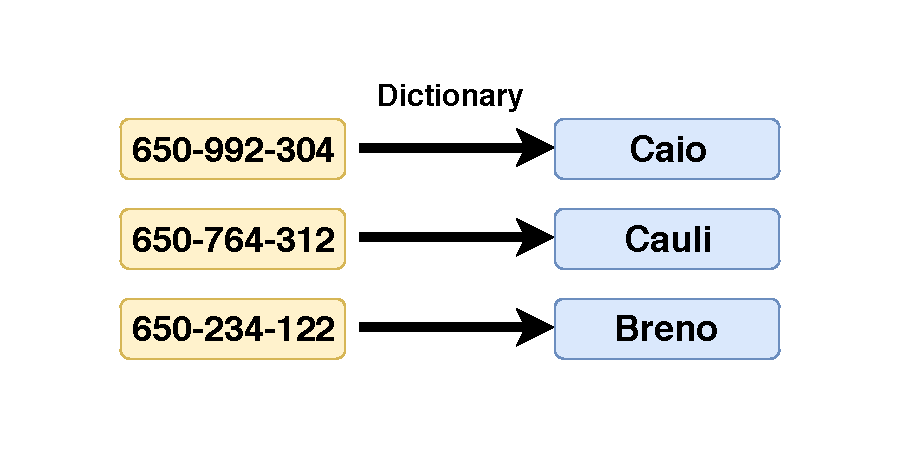
\includegraphics[width=12cm]{figuras/dictionary-example.pdf}
  \caption{Example of a dictionary that associates phone numbers to contact names. }
\end{figure}

Other use of a dictionary that we can think is to count the frequency that a certain number was called. One of the most used implementation of dictionaries is with a hash table. A key component in the implementation of a hash table is a hash function. This function usually takes the key of the key-value pair we want to add or update in the table and ``digest'' it into a number. That number is then used to identify the value, in this structure that we call hash table. In our example, the keys are phone numbers and the values are contact names.

An example of a hash function, that ``digest'' the phone numbers is the following: \\

\bigskip

\begin{figure}[h!]
  \centering
  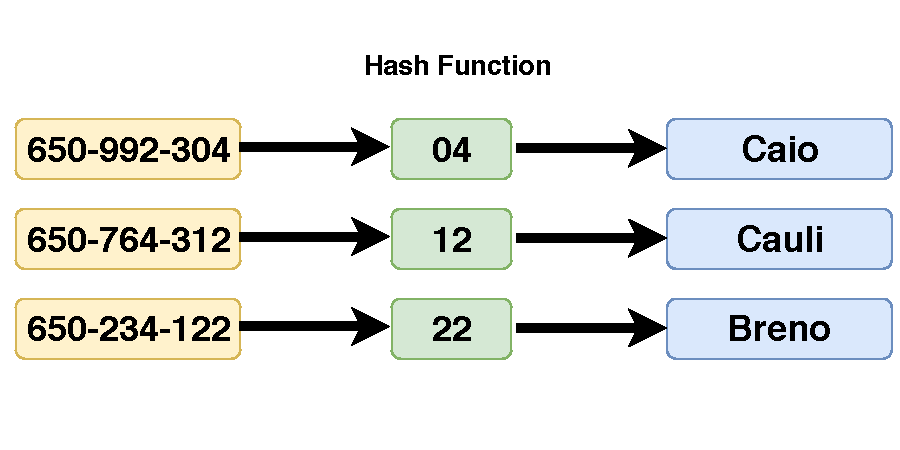
\includegraphics[width=12cm]{figuras/phone-hash-example.pdf}
  \caption{Example of a hash function hash function that just take the last 2 digits of the phone number }
\end{figure}

\medskip

As you can see this is a pretty simple function, it simply take the last 2 digits of each phone number. In this specific case, this is enough to uniquely identify each phone. We can imagine a function that can't uniquely identify each phone number, like getting just the last digit, in this case, Cauli's and Breno's numbers would have the same hash value, a collision in the table. Handling collisions in a hash table is a complete topic by itself, and it will be addressed in Chapter 3, Hash Tables. 

Handling collisions is actually a very important topic in hash tables and that is because the vast majority of hash functions will have collisions. To picture that we recall the ``Birthday Paradox'', that states that we only need 23 people in a room to have a chance greater than \( 50\% \) of 2 or more people having the same birthday. In Donald Knuth's famous book, The Art of Computer Programming (Vol. 3, Chapter 6.4) \citep{TAOCP3}, he uses as an example a function from a 31-element set to a 41-element set, and from about \( 10^{50} \) functions only about \( 10^{43} \) give distinct values for each argument, that is about 1 in every 10 million functions. This shows that we will have collisions more often than not, so knowing how to deal with it is a major problem that can not be neglected.

Hash functions and hash tables are among the most classic topics within computer science, yet is still one of the topics with most debate about what is state of the art. While the hash table was invented in 1953, widely discussed by Donald Knuth in his book, there are still many tweaks that can be made to boost its performance for specific use cases. One great example is F14, an open-source memory efficient hash table by Facebook \footnote{F14 is open sourced: \url{https://engineering.fb.com/developer-tools/f14/}}.

An example of lack of consensus in this area are the different hash functions and hash table implementations in different languages. There is no clear consensus on how to decide the size of a hash table, what are the trade-offs of the collision-resolution algorithms or even what defines a good hash function. Hopefully, we got years of research on the topic to study and present a view on the subject, and that is what I am presenting throughout this undergraduate thesis.

%% If you want it maybe interesting to cite Cassandra and other hash tables here.

\par

%% ------------------------------------------------------------------------- %%
\chapter{Hash Functions}
\label{cap:Hash Functions}

%% ------------------------------------------------------------------- %%
%\begin{itemize}
%\item Define Hash Function
%\item Give some examples of hash functions (Multiplicative / Remainder)
%\item Present Dragon Book metric and Evaluate hash functions
%\end{itemize}
%% ------------------------------------------------------------------- %%

Outside computer science, the word \textit{``hash''} in the English language means to ``chop'' or to ``mix'' something. This meaning is entirely related to what hash functions are supposed to do. Hash functions are functions that are used to map data of an arbitrary size to data of a fixed size \citep{HashFuncWiki}.

They have wide applications in computer science, being used in information and data security, compilers, distributed systems and hardcore algorithms. In this chapter we first define and explain the basics of a hash function, then we give an intuition in some metrics that tries to capture the idea of what is expected of a good hash function, as discussed in the famous \textit{``Red Dragon Book''} \citep{DragonBook} along with some reproduction of known results in the area.

The value extracted from the hash function for an object or key is usually called \textit{hash value} or simply \textit{value}. The hash value is in general, but not necessarily, smaller than the object that generated it. For example, we can have a hash function that takes Gigabytes or Terabytes files and return an 8 bytes hash value.

\begin{figure}[h!]
  \centering
  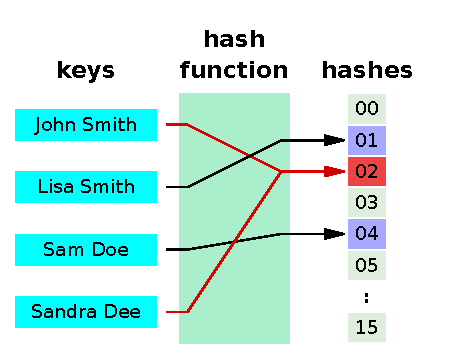
\includegraphics[width=6cm]{figuras/hash-function.pdf}
  \caption{Example of a hash function from string to 4 bit integer. Source: Wikipedia, Jorge Stolfi }
\end{figure}

\bigskip

\section{Definition}

A hash function over a set \( X \) a function \( H \) that takes an element \( x \) in \( X \) and associate to \( x \) a integer \( H(x) \) in the interval \( [0,M) \), for some integer \( M \). In symbols
\[ H: X \rightarrow [0, M) \]
When dealing with hash tables, \( X \) is the set of possible keys and \( M \) is the size of the table, which is usually just an array. Moreover, we saw earlier that hash functions are usually more useful when \( |X| > M \). This is the same definition used by Donald Knuth \citep{TAOCP3} and some articles \citep{RobinHoodHashing}. This definition makes sense for our purpose because we will be talking mostly about hash functions used in hash tables. In that case we want integers that will be indexes in an array (as we will see later on). In other cases we may see hash values as strings, like for when we hash an string for password storage or when we use a hash function in files for checking integrity (for when we are checking if two files are the same). For the goal of this thesis we will not be focusing on those functions, but it is important to notice that strings can also be easily associated to integers if we just look at their bytes.

For our purpose we are looking for a hash function that performs well for the construction of hash tables. Ideally, these functions should be fast to compute and minimizes the number of collisions. Depending on our goals we might want a different metric, for check-sums for example we may want a function that is very sensible to changes, and for passwords one that is very hard to find its inverse, those are so called cryptographic functions. For some collision resolution techniques, as we will see later, we may also want that the hash function disperse the values well too. Intuitively, a hash function should look like a random function having a given key as seed.

As written in Knuth's book, we know that it is theoretically impossible to create a hash function that generates true random data from non random data in actual file, but we can do pretty close to that or in some cases, even fewer collision than an uniformly random function. Knuth describes two specific methods for simple hash function, named \textit{division hashing} and \textit{multiplicative hashing} techniques. As the name suggests, the first is based on division operation and the former on multiplication operation.

\section{Division and Multiplicative Methods}

The \textit{division hashing} method maps an integer \( X \) associated to the data to its remainder modulo an integer \( M \). Supposing that we can represent the data as a non negative integer \( X \) the division hashing would be to choose a value M and the hashing function would be \( X \mod M \). The code would look as following:

\begin{lstlisting}
unsigned int divisionHashing(unsigned int X, unsigned int M) {
  return X % M;
}
\end{lstlisting}

A good hash function combines number theory, statistics and engineering and in general, large prime numbers tend to be a good value to \( M \), to avoid unwanted patterns or repetitions. One great example of this is if \( M \) is even, then the parity of hash value of \( X \) will match the parity of \( X \) (which will cause a bad distribution). The same pattern will happen in different intervals for different powers of \( 2 \).

For \textit{multiplicative hashing}, let's first suppose once more that we can represent the data as a non-negative integer \( X \) and we have chosen a constant \( S \), where \( 0 < S < 1 \). Then we multiply \( X \) by \( S \) and extract the fractional part of \( X \times S \), that is \( X \times S \mod  1 \). We can calculate that by doing: \( X \times S - \lfloor X \times S \rfloor \). Then we multiply that value, that will be between 0 and 1, by \( M \). The code of what was described above would look as following:

\medskip

\begin{lstlisting}
unsigned int multiplicativeHashing(unsigned int X,
                                   double S,
                                   unsigned int M) {
  double alpha = (double) X * S - floor((double) X * S);
  return (unsigned int) floor(alpha * (double) M);
}
\end{lstlisting}

In Knuth's book he describes \( S \) as being an integer \( A \) divided by \( w \), where \( w \) is the size of a ``word'' in our computer. He restricts \( A \) to be relatively prime to \( w \). That definition is often useful if you want to retrieve a value \( Y \) for a given hash value \( F \). This can be done via Bezout theorem \citep{TAOCP3}. It is good to note here that if \( H(X) = F \) and \( H(Y) = F \), \( X \) is not necessarily equal to \( Y \), as two different keys can have the same hash value.

\section{Hashing Strings}

We have many ways of converting non numerical data to non negative integers. In the end, it is all just a sequence bytes, that when read in a specific way form another type of data, such as images or strings. For example, one way of transforming a string to a non-negative integer is summing the ASCII value of its characters. The C++14 code for that would look as following:

\begin{lstlisting}
unsigned int stringToInteger(string str) {
  unsigned int hashValue = 0;
  for (char c : str) {
    hashValue += (int) c;
  }
  return hashValue;
}
\end{lstlisting}

We always use unsigned integers for our non negative integer calculations due to the natural modulo operation of it on overflow cases. It is equivalent to having a \( \mod \ 2^{32} \) every time it overflows, as we only look at the leading 32 bits. We can also use XOR function to mix numbers together. 

There is also a very common type of hash functions that tend to work pretty well for strings \citep{DragonHashFunc}. It is a ``superset'' of multiplicative hash functions, or a generalization. The C++14 code would look as following:

\begin{lstlisting}
unsigned int hashForString(string str,
                           unsigned int initialValue,
                           unsigned int multiplier,
                           unsigned int modulo) {
  unsigned int hash = initialValue;
  for (char c : str) {
    hash = (multiplier * hash + (int)c);
  }
  return hash % modulo;
}
\end{lstlisting}

The above function is very common for string hashing, and by just choosing a different initial value and multiplier we can have completely different hash functions. Although using summing or using XOR to combine the previous hash value with the new character usually don't provide much difference, with XOR operation we do not need to worry about overflow. Some values are of known hash functions, for example with \texttt{multiplier = 33} and \texttt{initialValue = 5381} generates \textit{Bernstein hash djb2} \citep{BernsteinHash} or \texttt{multiplier = 31} and \texttt{initialValue = 0} generates \textit{Kernighan and Ritchie's hash} \citep{KernighanHash}. Those are famous functions and their values are not chosen randomly, as there are some factors that maximizes the chance of producing a good hash function, where good means low collision rate and fast computation. Those factors are:

\begin{itemize}
\item The multiplier should be bigger than the size of the alphabet, in our case usually 26 for English words or 256 for ASCII. That is the case because if it is smaller we can have wrong matches easier. For example, suppose that \texttt{multiplier = 10} and \texttt{initialValue = 0}, we have \( H('ABA') = H('AAK') = 7225 \) before taking the modulo operation.

\item The multiplication by the multiplier should be easy to compute with simple operations, such as bitwise operations and adding. That is quite intuitive as we want a hash function that is fast to calculate. 

\item The multiplier should be coprime with the modulo. That is because if not we will ``cycle'' hashes at a greater rate than the modulo (We can use some modular arithmetic to prove that). Usually prime numbers tend to be good multipliers.
\end{itemize}

\section{Quality of a Hash Functions}

Now that we know some good templates for producing hash functions lets try to find a concrete metric or formula that measures the quality of a hash function. Fortunately, the famous book Compilers: Principles, Techniques, and Tools, also known as ``Red Dragon Book'' \citep{DragonBook}, has already proposed a quantity to measure the quality of a hash function. The formula gives this quantity:
\[ \mathlarger{\sum}_{j = 0}^{m - 1} \frac{b_j(b_j + 1)/2}{ (n/2m)(n + 2m - 1) }, \]
where \( n \) is the number of keys, \( m \) is the number of total slots and \( b_j \) is the number of keys in the \( j \)-th slot. The intuition for the numerator is that it represents the number of operations we will need to perform to find each element of the table. For example, we need 1 operation to find the first element, 2 to find the second, and so on. That means that we will end up with an arithmetic progression. We know that a hash function that distributes the keys according to an uniformly random distribution has expected bucket size of \( n / m \), so we can calculate that the expected value of the numerator formula is \( (n/2m)(n + 2m - 1) \). So that gives us a ratio of collisions (thinking just about operations to access a value) of ``our'' hash function with an ``ideal'' function. That means that a value close to \( 1.00 \) of the above formula is good, and values below to \( 1.00 \) means that we had less conflicts than an uniformly distributed random function.

From common data as used in Dragon Book and Strchr website \citep{DragonHashFunc} I will reproduce some tests with the previously cited hash functions.

\begin{figure}[h!]
  \centering
  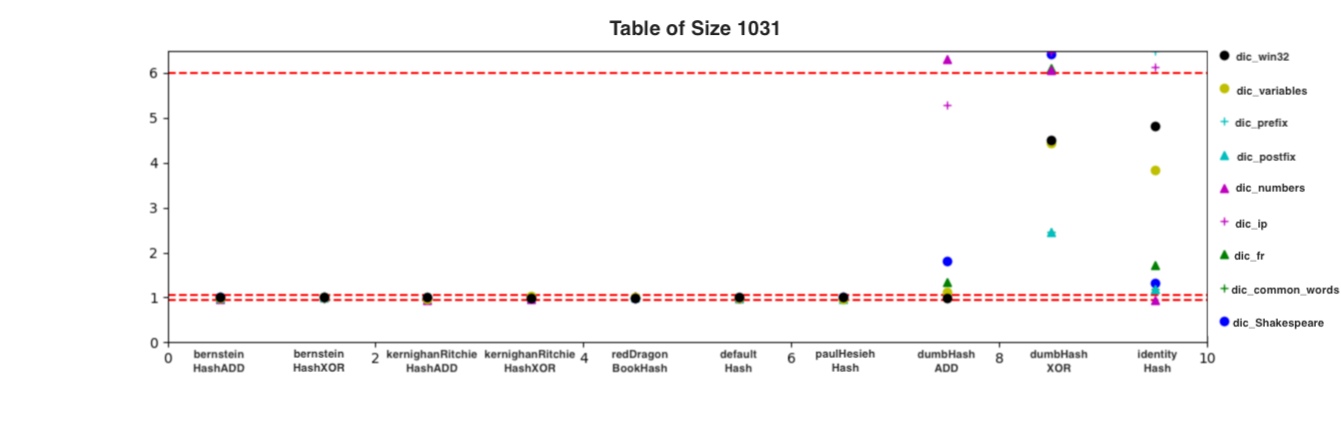
\includegraphics[width=14cm]{figuras/1031HashFunc.png}
  \caption{Functions tested against a ``small'' table}
\end{figure}

\medskip

\begin{figure}[h!]
  \centering
  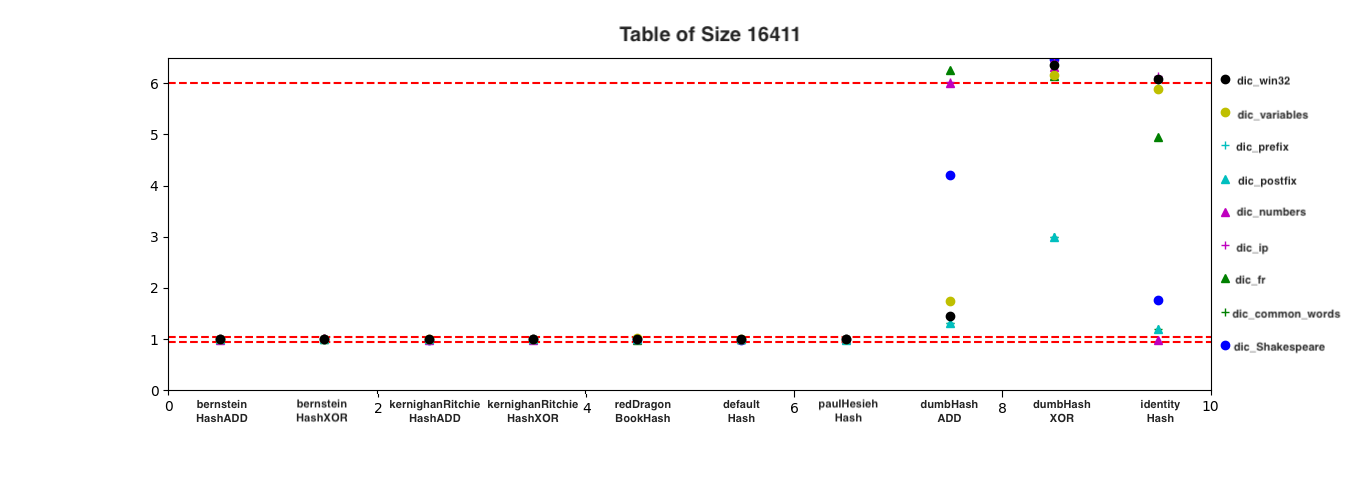
\includegraphics[width=14cm]{figuras/16411HashFunc.png}
  \caption{Functions tested against a ``medium'' sized table}
\end{figure}

\medskip

\begin{figure}[h!]
  \centering
  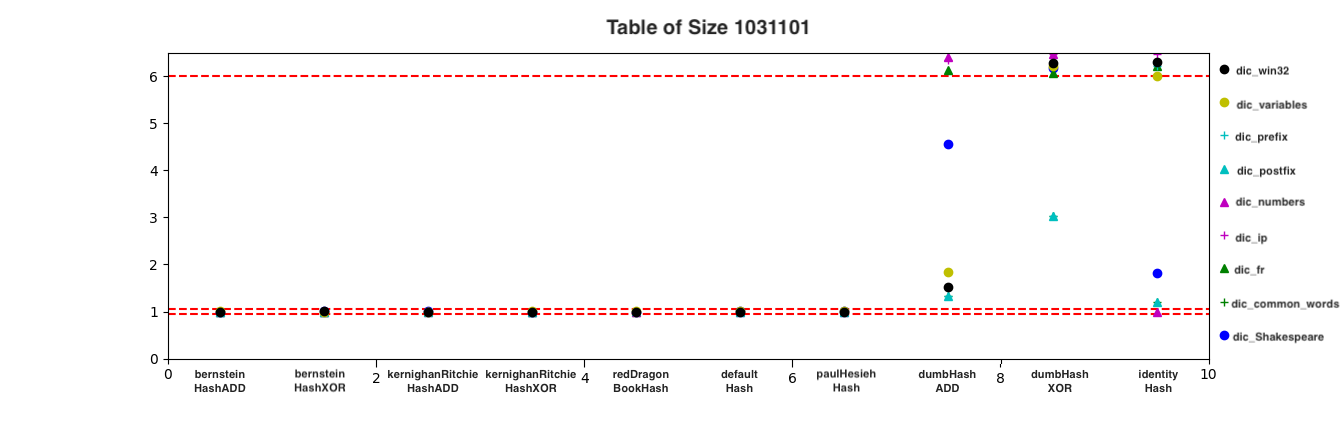
\includegraphics[width=14cm]{figuras/1031101HashFunc.png}
  \caption{Functions tested against a ``large'' table}
\end{figure}

\medskip

The results are shown in the same way displayed in the Red Dragon Book, with hash functions in the \( x \) axis and the ratio displayed in the \( y \) axis, with different identification for each file. We consider three sizes of tables to to count collisions, a ``small'', ``medium'' and a ``large'' table, the small table having a load factor (The percentage of the table occupied) of approximately \( \sim 0.5 \), the medium with \( \sim 0.05 \) and large with \( \sim 0.005 \). It's assumed that the modulo is not the responsibility of the hash function, so all hash functions return values from 0 to \( 2^{32} - 1 \), and the modulo is taken depending on the size of the table. From that we can already see that the load factor doesn't make a good hash function bad, but expose problems of ``bad'' hash functions in some cases. 

Another fact that it is important to notice from the graph is the red dotted lines. The top one is the ``Upper'' threshold, which results greater than 6 are just considered ``Big'', as in some cases the ratio exploded to values up to 200. The lower 2 red lines are in \( y = 1.05 \) and \( y = 0.95 \) which is the interval that we consider a hash function to have ``Good'' values. 

The tests were made with 10 different hash functions, tested against 9 different files (Provided by strchr website). All of the code used to test this can be found in the github repo \citep{GithubRepo}. The 10 hash functions are the following:

\begin{itemize}
\item \textbf{bernsteinHashADD}: The Bernstein hash function described earlier. We use the given hash template adding the elements. The multiplier is 33 and initial value is 5381. In the end we XOR the bits of the hash with itself shifted 16 to the right (That is half of the bits with our implementation).
  
\item \textbf{bernsteinHashXOR}: The same as above but substituting the first adding operator by the XOR operation.

\item \textbf{kernighanRitchieHashADD} The Kernighan and Ritchie Hash function described earlier. We use the given hash template adding the elements. The multiplier is 31 and initial value is 0.

\item \textbf{kernighanRitchieHashXOR} The same as above but substituting the first adding operator by the XOR operation.

\item \textbf{redDragonBookHash} The hash function tested in the Red Dragon Book. It is described as x65599 in the book.

\item \textbf{defaultHash} The default hash function of C++ standard template library.

\item \textbf{paulHesiehHash} A fast hash function described by Paul Hesieh. It is fast to calculate and more complex than Knuth multiplicative or division Hashing.
  
\item \textbf{dumbHashADD} A hash function that simply add all characters.

\item \textbf{dumbHashXOR} A hash function that simply XOR all characters.

\item \textbf{identityHash} A hash function that takes the first 4 bytes of the string.  
\end{itemize}

We have a variety of hash functions, with all being considered ``fast'' hash functions. The files tested include common words in English and french, strings of some IP values, numbers, common variable names and words with common prefix and suffix.

First thing we can notice from those graphs is that changing the ADD function to XOR doesn't make a good multiplicative hash function bad. Both are actually ``Equivalent'' given that we are also multiplying the values. For \texttt{dumbHashADD} and \texttt{dumbHashXOR} we can see clear differences, with \texttt{dumbHashXOR} being clearly worse. This can be explained by the cancellation property of XOR. We can see this example on the hash of this IP below:

\texttt{dumbHashXOR('168.1.1.0') = dumbHashXOR('168.2.2.0') = dumbHashXOR('124.6.8.0')}

We can see that many different IPs have the same hash value. More than that, XOR don't increase the number of bits, so all the hashes will be of just 1 byte.

Other thing that we can notice is that ``identity'' hash is good or perfect in some cases. One obvious case that ``identity'' function works perfectly is for numbers as we will have 0 collisions. Some languages, like Python 3, use the identity function to calculate hash for integers, as it is very fast and produces no collisions. But we can see that for other cases, such as common prefix, it works terrible as we just get the first 4 bytes.

The most common multiplicative hash functions tend to work similarly well, being reasonably close to an uniformly random function (that is our ``ideal'' hash function) in all cases.

As we can see, we don't need a lot of complexity to make a good hash function for a hash table. We have some functions working better for some specific case, like identity function working well for numbers, but general functions already work well enough.

One thing that is important to note here is that hash function is a very vast topic, and here we just covered hash functions related to hash tables. Hash functions have applications in distributed systems (consistent hashing), database indexing, caching, compilers (Red Dragon Book) and cryptography. Each application has different requirements and make some hash functions better than others.
\par


%% ------------------------------------------------------------------------- %%
\chapter{Hash Tables}
\label{cap:Hash Tables}

%% ------------------------------------------------------------------- %%
%\begin{itemize}
%\item Define hash table and its operations
%\item Open Addressing Strategies (Linear Probing, Quadratic Probing, ...)
%\item Chaining Strategy (Simple Chaining, Move-to-front ...)
%\item Load factor and resizing/rehashing the table
%\end{itemize}
%% ------------------------------------------------------------------- %%


Hash tables or hash maps is one of the most used applications of hash functions. It is actually so used in computer science that is almost impossible to talk about one without mentioning the other. This data structure consists in associating a \textit{key} to a \textit{value} in a table. That is, given a \textit{key}, it can retrieve the  \textit{value} for it.

It is one of the possible, and many times considered the best, implementations of a dictionary. It has to implement the \texttt{insert}, \texttt{find} and \texttt{remove} operations, that can be accessed from outside the dictionary. It usually implements a lot of other private methods. 

This data structure is usually considered very useful among software engineers and computer scientists, although it usually has a linear worst case cost for retrieving, inserting and deleting a key-value pair. That is because hash tables usually have a constant average cost for those operations.

Moreover, when talking about hash tables we have the problem of key collision, that is when two keys map to the same hash value. As we saw in the previous chapter, collisions are more common than not, so collision resolution is a critical problem. To solve that problem, we have several techniques that involve different trade-offs. Those techniques are usually divided into two main categories, open addressing and separate chaining. Other problem to consider regarding this data structure is when to resize the hash table, to minimize the chance of collision and the use o memory. For this last one we usually consider a load factor, \( \alpha \), that is the ratio of keys with the available slots in the table.

\newpage

Also, hash tables can be easily abstracted to hash sets, commonly used to store a set of elements and check whether an element is in the set. We can abstract hash sets to a hash table always with an empty value. Hash sets are one of the common ways to implement sets in programming languages, like unordered\_set from C++14.

It is also important to notice that hash tables have applications in different areas of computer science also, like compilers, caches and database indexing.


\begin{figure}[h!]
  \centering
  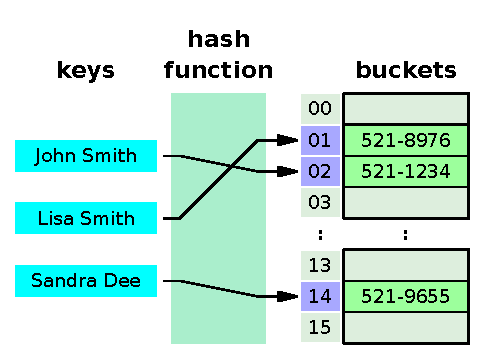
\includegraphics[width=12cm]{figuras/hash-table.pdf}
  \caption{Example of a hash table from string to string, more specifically name to phone number. Source: Wikipedia, Jorge Stolfi }
  \label{fig:hashTable}
\end{figure}

In the above figure (\ref{fig:hashTable}), we can see an example of a hash function that matches names of people to phone numbers, as we saw in the first chapter. This table has no collisions, and we can see that, for example, ``Jhon Smith'' has a hash value of 2 and his value in the table is ``521-1234''. That is we associated a names with phone numbers.

\newpage

\section{No collision open addressing hash table }

To start let's give an example of a hash table that has a perfect hash function, that is a function from \( X \) to \( [0, M) \) with no collisions from the used keys. For that example we use open addressing, that basically means that all data will be contained in an array (that is, the whole table). The operations \texttt{insert}, \texttt{find} and \texttt{remove} would be very easy to implement. For the sake of simplicity, we will assume all the keys are strings and values are integers. To start lets look at this simple class with dummy methods:

\begin{lstlisting}
class HashTable {
   vector< pair<string, int> > table;
   int m, n;
   
   HashTable() {
      m = 16;
      table.resize(m);
      n = 0;
   }

   unsigned int hashFunction(string s) {}
   
   void insert(string key, int value) {}

   int find(string key) {}

   void remove(string key) {}

private:
   double alpha = 1;
   void resizeIfNecessary() {}
}
\end{lstlisting}

As we can see it is pretty simple. The constructor builds a table of size \( 16 \), and we can assume a dynamic resizing every time the table is full. Later on we will see that this means that we resize every time the load factor, \( \alpha \), is equal to \( 1.00 \). We also can note that at the table part we are storing a pair of key and value, not just value. This is because we may want to retrieve all pairs of the table (like in a regular dictionary). The pairs are usually unordered (If they are not ordered by chance \dots). Actually, if one needs the set of keys sorted by total order, very likely hash tables are not the appropriate data structure. We will skip the implementation of hashFunction, as we already saw plenty of it in the last chapter, so we will go right in for the implementation of \texttt{insert}:

\begin{lstlisting}
void insert(string key, int value) {
  resizeIfNecessary();
  unsigned int idx = hashFunction(key);
  table[idx] = pair<string, int>(key, value);
  n++;
}
\end{lstlisting}

That is pretty simple, that is mostly because we will assume that we will never have a collision, so we just put the key on the position returned by the hash function. The method \texttt{find} is implemented as following:

\begin{lstlisting}
int find(string key) {
  unsigned int idx = hashFunction(key);
  if (table[idx].first == key)
    return table[idx].second;
  return 0;
}
\end{lstlisting}

Also very simple, we always know the value will be in position returned by idx. The \texttt{remove} will be of the same simplicity, as following:

\begin{lstlisting}
void remove(string key) {
  unsigned int idx = hashFunction(key);
  table[idx].first = pair<string, int>("", 0);
  n--;
}
\end{lstlisting}

Here we make the assumption that an empty position has an empty string. We could also carry a boolean, usually called a tombstone, to check if the position is occupied or not. If the hash function is perfect, than the insert, find and delete operations can be performed in constant time and linear space.

\section{Open addressing}

We can define open addressing in a general way as a hash table algorithm where the data always stay within the same vector. So, in the case of a collision, we need to define a systematic way to traverse the table. The sequence of elements we need to traverse when we have a collision is called \textit{``Probe sequence''}. With that our hash function would change to the following:
\[ h(x, i) \],
where \( x \) is our key and \( i \) is the probe sequence number. So every time we have a collision in \( h(x, i) \) we can simply go to \( h(x, i + 1) \). Given that, lets look into some different probe sequences.

\section{Linear Probing}

Linear probing is one of the most simple an practical probe sequences known. The probe sequence is basically:
\[ h(x, i) = (H(x) + i) ~\mathrm{mod}~ M \],
where \( M \) is the table size. That is a very simple probe sequence with not much secret on it. To implement the \texttt{insert} we can do the following:

\begin{lstlisting}
void insert(string key, int value) {
  resizeIfNecessary();
  unsigned int idx = hashFunction(key);
  while (table[idx] != pair<string, int>("", 0))
    idx = (idx + 1) % m;      
  table[idx] = pair<string, int>(key, value);
  n++;
}
\end{lstlisting}

That assumes that \texttt{pair<string, int>("", 0)} is the empty position, and performs a linear search until it finds one empty position to put the new (key, value) pair. The implementation of \texttt{find} is very similar:

\newpage

\begin{lstlisting}
int find(string key) {
  unsigned int idx = hashFunction(key);
  while (table[idx] != pair<string, int>("", 0)) {
    if (table[idx].first == key) 
      return table[idx].second;
    idx = (idx + 1) % m;
  }
  return 0; // Default value
}
\end{lstlisting}

It performs a linear search until it finds the element. If the key is not found the function returns a default value, that in our case is 0. 

For removal, we have the problem that we cannot leave ``holes'' in our table. That will be discussed more in depth later on the section ``How to delete an entry''. For now we will remove the element, and reinsert the key-value pairs that come right after it:

\begin{lstlisting}
void remove(string key) {
  unsigned int idx = hashFunction(key);
  while (table[idx] != pair<string, int>("", 0)) {
    if (table[idx].first == key) 
      break;
      idx = (idx + 1) % m;
  }
    
  if (table[idx].first == key) {
    table[idx] = pair<string, int>("", 0);
    vector< pair<string, int> > toRehash;
    int j = (idx + 1) % m;
    while (table[j] != pair<string, int>("", 0)) {
      toRehash.push_back(table[j]);
      table[j] = pair<string, int>("", 0);
      j = (j + 1) % m;
    }
    for (auto p : toRehash) {
      insert(p.first, p.second);
    }
    n--;
  }  
}
\end{lstlisting}

With that, the three operations have linear time complexity in the worst case. As we saw, we know hash functions that are considered good, with a rate of collision very close to an uniformly random function. Those functions will leave us with an expected constant time complexity for those operations, and we will see later on that in practice it is much faster than linear access. Another great benefit that linear probing has, specially when compared to other collision resolution strategies, is locality and cache friendliness.

However linear probing has the problem of clustering, that is long chains of occupied positions. This generates a greater problem, as long chains are only expected to get longer and longer. This can get worse if the hash function is not too sensitive to changes, having a lot of sequential hash values. 

\section{Quadratic Probing}

Another strategy for resolving collisions is quadratic probing. In this case, the probe sequence can be defined as:
\[ h(x, i) = (H(x) + i^2) \mod M \]
That solves the problem of having sequential hash values. The implementation of quadratic probing is very similar to the implementation of linear probing, with the exception that instead of adding one for each step we can keep the initial value and add the square of a counter.

However, quadratic probing doesn't solve the problem of clustering. Long chains are still expected to get longer and longer, the only difference is that the positions that lead to a longer chain are better distributed in the table. Another thing to notice is that quadratic probing has a worse locality and cache friendliness than linear probing. 

\section{Double Hashing}

As we saw the two strategies above have the problem of clustering, due to the fact that the sequences are the same for all keys. For that reason double hashing is a very good approach for open addressing. Double hashing probe sequence can be defined as following:
\[ h(x, i) = (H_1(x) + i * H_2(x)) \mod M \],
where \( H_1 \) and \( H_2 \) are two distinct hash functions. In that way not only the initial hash value will depend on \( x \), but it's probe sequence offset (that is, the number of slots between \(h(x, i) \) and \(h(x, i + 1) \)) will too. The implementation of double hashing is very similar to both quadratic and linear probing, except that we sum a different offset.

These last three implementations of hash table give us linear time worst case complexity for all operations and constant time expected time complexity under the simple uniform hashing assumption.

\section{Robin Hood Hashing}

Robin Hood Hashing is an optimization technique regarding collision resolution with open addressing. It should be paired with Linear Probing, Quadratic Probing or Double Hashing, but usually it is paired with linear probing due to it is good locality and cache friendliness. It is basic is that it minimizes the distance of each key from its ``home Slot'', that is, its initial hash value position. \citep{RobinHoodHashing}. Also, Robin Hood hashing is one of the few open addressing strategies to be built-in in hash tables of some languages, such as Rust.

In order to minimize the distance from each key from its home slot, Robin Hood hashing uses a concept that is called Probe Sequence Length, or PSL, of a key-value pair. The PSL of a key-value pair is the number of probes required to find that pair. For that reason we need to define a new class to store in our table, that we will call \texttt{Node}:

\begin{lstlisting}
class Node {
public:
   string key;
   int value;
   unsigned int PSL;   
   Node(string K = "", int V = 0, unsigned int P = 0):
      key(K), value(V), PSL(P) {}

   bool operator == (const Node& ot) {
      return key == ot.key && value == ot.value && PSL == ot.PSL;
   }
   bool operator != (const Node& ot) {
      return key != ot.key || value != ot.value || PSL != ot.PSL;
   }
};

const Node defaultNode = Node();
\end{lstlisting}

\texttt{Node} is a very simple class that stores a key, a value and an unsigned integer that is the PSL. The main idea around Robin Hood hashing it to move the Nodes with a low PSL in favor of Nodes with a high PSL. We can think of Nodes with a high PSL as poor, because we take longer to find it, and Nodes with a low PSL as rich because we can find them faster. For that reason the algorithm is called Robin Hood Hashing \citep{RobinHoodHashing}.

As explained when inserting an element we first look for an empty position. While searching for it, we check whether the \texttt{Node} that is in the way has a lower PSL than the Node that we are inserting, and if that is the case we swap them, securing a position for the current Node and move the other node forward. The implementation of this algorithm using Linear Probing would be the following:

\begin{lstlisting}
void insert(string key, int value) {
  resizeIfNecessary();
  unsigned int idx = hashFunction(key);
  Node toInsert = Node(key, value, 0);
  while (table[idx] != defaultNode) {
    if (toInsert.PSL > table[idx].PSL)
      swap(toInsert, table[idx]);         
    idx = (idx + 1) % m;
    toInsert.PSL++;
  }
  table[idx] = toInsert;
  n++;
}
\end{lstlisting}

For the \texttt{find} method we can use different lookup techniques. Here we will focus on the lookup that is most similar with linear probing, but with a tweak that will make finding that keys are not present faster. While searching for a key, we can calculate what the PSL of that key would be if were inserted, and if we find a Node with a greater PSL that means the pair is not present. That is because all Nodes after it will also have a PSL greater than the current PSL. The implementation of what was described above would be the following:

\newpage

\begin{lstlisting}
int find(string key) {
  unsigned int idx = hashFunction(key);
  unsigned int curPSL = 0;
  while (table[idx] != defaultNode) {
    if (table[idx].key == key) 
      return table[idx].value;
    // If the key were inserted it would be before this Node.
    if (table[idx].PSL > curPSL)
      break; 
    idx = (idx + 1) % m;
    curPSL++;
  }
  return 0; // Default value
}
\end{lstlisting}

For the removal we can apply \textit{backward shifting}. Although this will be discussed more in depth in the ``How to delete an entry'' section, this approach is unique to robin hood hashing and has a better performance than rehashing.

\textit{Backward shifting} consists in first clearing out the slot that contains the key to be removed, then shifting the following keys one step back until a Node with 0 PSL or an empty slot is encountered. The code for that would be the following:

\begin{lstlisting}
void remove(string key) {
  unsigned int idx = hashFunction(key);
  while (table[idx] != defaultNode) {
    if (table[idx].key == key) 
      break;
    idx = (idx + 1) % m;
  }
  if (table[idx].key == key) {
    table[idx] = defaultNode;
    while (table[(idx + 1) % m] != defaultNode &&
           table[(idx + 1) % m].PSL != 0) {
      swap(table[idx], table[(idx + 1) % m]);
      table[idx].PSL--;
      idx = (idx + 1) % m;
    }
    n--;
  }
}
\end{lstlisting}

We can always do that because the keys are always sorted according to the their home slot (That is, the first Node with PSL that is 0 that comes before them).

The worst time complexity of all operations is linear and the expected time complexity is constant. The expected length of the longest PSL in a full table is \( \log n \).
\section{Cuckoo Hashing}

Another well known strategy for collision resolution in open addressing is Cuckoo Hashing. It is a different strategy regarding the previous ones because it uses more than one array, usually two, but up to any number of arrays, to perform collision resolution. It is usually classified as open addressing because each slot can hold up to one key-value pair. For this explanation let's assume that we are using two arrays. Cuckoo hashing requires also one hash function per array used, in our case two hash functions.

%% Image representing cuckoo hashing

For the insertion of cuckoo hashing we try to insert the key in the first table and if a collision occurs we swap the key value pair that we are trying to insert with the element that is currently on the table and then try to insert it on the next array. If a collision occurs in the other array we swap the pairs and try again on the next one, until we find an empty position or we reach a certain threshold. The threshold is important because we can have cycles.

%% Image Representing insertion.

The code for the algorithm described above is the following:

\begin{lstlisting}
void insert(string key, int value) {
  resizeIfNecessary();
  unsigned int j = 0, it = 0;
  unsigned int idx = hashFunction(key, j), lim = maxLoop();
  pair<string, int> toInsert = pair<string, int>(key, value);
  while (table[j][idx] != pair<string, int>("", 0) && it < lim) {
    swap(table[j][idx], toInsert);
    j = (j + 1) % numTables;
    idx = hashFunction(toInsert.first, j);
    it++;
  }
  if (it == lim)
    resize();
  table[j][idx] = toInsert;
  n++;
}
\end{lstlisting}

This gives a very strong property to this collision resolution approach, that is every key value pair will be in its corresponding position in exactly one of the arrays. And this will give constant Lookup and Removal time. 

In order to find a key value pair we just need to look if the key value pair is present in one of the tables. The code is the following:

\begin{lstlisting}
int find(string key) {
  for (unsigned int j = 0; j < numTables; j++) {
    unsigned int idx = hashFunction(key, j);
    if (table[j][idx].first == key)
      return table[j][idx].second;
  }
  return 0;
}
\end{lstlisting}

For removal we can simply erase the key value pair from the table, as no key value pair affect the lookup of any other pair. The code is the following:

\begin{lstlisting}
void remove(string key) {
  for (unsigned int j = 0; j < numTables; j++) {
    unsigned int idx = hashFunction(key, j);
    if (table[j][idx].first == key) {
      table[j][idx] = pair<string, int>("", 0);
      n--;
    }
  }
}
\end{lstlisting}

Besides the amazing property of guaranteed constant lookup and removal, Cuckoo hashing has the problem of cycles during insertion, which can cause unwanted rehashes. To deal with that, many implementations also use a stash to keep a constant amount of elements in case the threshold is reached. A stash is a sort of ``bin'' of fixed size that we put key-value pairs that failed insertion, and during lookup we would also need to look at the stash.

\section{Coalesced Hashing}

Another well known strategy, described in Donald Knuth book \citep{TAOCP3}, is Coalesced Hashing. Although without much advantages in contrast with previous strategies, coalesced hashing condenses the hash table well in memory and is very similar to Chaining Hashing, our next topic.

The main idea of coalesced hashing is to add a new parameter to our key value pairs in the table, called next. That would create linked lists in the table in case we have a collision. To find the next element in case a collision we can find the first free bucket looking to the array in reverse order. The function to find the next free bucket is the following:

\begin{lstlisting}
int nextFreeBucket() {
  for (int i = m - 1; i >= 0; i--) {
    if (table[i].isDefaultNode())
      return (unsigned int)i;
    }
  return -1; // error
}
\end{lstlisting}

To insert an element, in case of a collision, we need to traverse the linked list beginning on the bucket that the key hashes to until the end. Then we add a new Node to the end of the linked list, pointing to the next free bucket. The complete code of the insertion algorithm will be shown later on.

To lookup for an element, we can traverse the linked list until we find a matching Node. The code for the find method would be the following:

\begin{lstlisting}
int find(string key) {
  unsigned int idx = hashFunction(key);
  while (idx != -1) {
    if (table[idx].key == key) 
      return table[idx].value;
    idx = table[idx].next;         
  }    
  return 0;
}
\end{lstlisting}

Removing a node in coalesced hashing is very difficult, as many other nodes can depend on it. For this reason the best way to delete an element in coalesced hashing is by using a strategy that is known as tombstoning. The idea of this strategy is to put a placeholder value, that will be considered as occupied by the find method but as free by the insertion method. The code for that would be the following:

\begin{lstlisting}
void remove(string key) {
  unsigned int idx = hashFunction(key);
  while (idx != -1) {
    if (table[idx].key == key) 
      break;
    idx = table[idx].next;         
  }
  if (table[idx].key == key) {
    table[idx].transformTombstone();
    n--;
  }
}
\end{lstlisting}

For this reason, the insertion method explained earlier on would have to be a little bit different, considering tombstones. The code would look like the following:

\begin{lstlisting}
void insert(string key, int value) {
  resizeIfNecessary();
  unsigned int idx = hashFunction(key);
  Node toInsert = Node(key, value, -1);
  if (!table[idx].isDefaultNode()) {
    while (table[idx].next != -1 && !table[idx].isTombstone())
      idx = table[idx].next; 
    if (!table[idx].isTombstone()) {
      table[idx].next = nextFreeBucket();
      idx = table[idx].next;
    }
  }
  table[idx] = toInsert;
  n++;
}
\end{lstlisting}

\section{Chaining hashing}

Chaining hashing, also known as closed addressing, is the implementation of a hash table using a container, usually called bucket, to store the (key, value) pairs with a given hash. On this implementation, each bucket of the table is a linked list, that will carry the key value pair in our case. We deal with collisions with this implementation by adding a new node to the start of the list.

This implementation is considered simpler than open addressing, usually because the way of dealing with collisions is clearer. Also it is less system dependent if we consider performance (as we saw one of the key advantages of open addressing is that it is cache friendly). That is one of the key reasons that C++ uses chaining hashing for its default implementation of unordered\_hash \citep{HashTableProposal}.

Below we will discuss an implementation of chaining hashing.

\section{Simple Chaining Hashing Algorithm}

For this chaining hashing implementation we will use C++14 STL data structure list as our container. list is a doubly linked list. For our \texttt{insert} we can implement it in the following way:

\begin{lstlisting}
void insert(string key, int value) {
  resizeIfNecessary();
  unsigned int idx = hashFunction(key);      
  table[idx].emplace_front(key, value);
  n++;
}
\end{lstlisting}

As we can see it is a very simple implementation, we just push a new element in the front of the list pointed in the idx. As before we add the counter of elements in the list and call resizeIfNcessary().

For \texttt{find} we can implement in the following way:

\begin{lstlisting}
int find(string key) {
  unsigned int idx = hashFunction(key);
  auto it = find_if(table[idx].begin(), table[idx].end(),
                    [&key](auto& kv) { return kv.first == key; });
  if (it != table[idx].end())
    return it->second;
  return 0;
}
\end{lstlisting}

That implementation is very succinct but uses some of the features of C++14 (such as generic lambdas). For \texttt{erase} we can implement in a very similar fashion:

\begin{lstlisting}
void remove(string key) {
  unsigned int idx = hashFunction(key);
  auto it = find_if(table[idx].begin(), table[idx].end(),
                    [&key](auto& kv) { return kv.first == key; });
  if (it != table[idx].end()) {
    table[idx].erase(it);
    n--;
  }
}
\end{lstlisting}

As we can see, with linked list it is clearly easier to erase an element. 

The naive algorithm of chaining hashing with a linked list gives linear worst time complexity for all operations and constant expected time complexity under the assumption of simple uniform hashing. 

% THINK ABOUT PUTTING THAT.

%One interesting thing to notice regarding chaining hashing implementation in C++ is that we may have a greater performance with implementations using vector instead of list, because of the better locality of vector.

\section{Move to front}

One great optimization to chaining hashing is every time you execute the \texttt{find} method to move to the beginning of the container the element that was found. That will keep in the beginning of the container the elements that are searched the most. As in many applications we can apply the 80 / 20 rule this greatly helps in time performance. The 80 / 20 rule is basically the idea that usually, 20\% of the keys will represent 80\% of the searches, this rule is also cited by Knuth \citep{TAOCP3}.

If our container is a linked list we can easily adapt the above implementation to move to front every time we search an element, with const time complexity cost. The implementation of \texttt{find} would be the following:

\begin{lstlisting}
int find(string key) {
  unsigned int idx = hashFunction(key);
  auto it = find_if(table[idx].begin(), table[idx].end(),
                    [&key](auto& kv) { return kv.first == key; });
  if (it != table[idx].end()) {
    if (it != table[idx].begin()) {
      table[idx].splice(table[idx].begin(), table[idx],
                        it, next(it));
    }
    return it->second;
  }
  return 0;
}
\end{lstlisting}

Here we are using the \texttt{splice} method of list C++ standard library to move an element inside a list. This still keeps the complexity of \texttt{find} in linear worst time and constant expected time. It is important to notice here that if our container wasn't a linked list we could take longer than constant time to move it to front.


\section{How to delete an entry}

In open addressing deleting an entry is considered hard by many of the collision resolution methods. Between clearing the entry and rehashing, clearing the entry and shifting the elements back or using tombstone, tombstone is usually considered the fastest approach due to its laziness.
The problem with tombstones is that it can make the table ``dirty'' if we have a high number of deletions, making lookups or insertions slower. So one suggestion is to rehash your table in the case of a high number of tombstones.

In contrast, deleting an entry in chaining hashing is delegated to the container that contains the key. That is, if we have a linked list as our container we just delegate the deletion to it. This is much easier is create less problems than open addressing deletion. That is one of the reasons why chaining hashing is usually chosen for default hash table implementation in many languages, like in C++ \citep{UnorderedMapDiscussion}.

\section{When to resize an array}

In open addressing the load factor to resize a hash table can't be greater than 1.0, because the table can't have more elements than its capacity. That is not true for chaining hashing as we will see later on. A good load factor depends on several factors, such as the strategy used. Some strategies are more ``permissive'' of a load factor closer to 1, Robin Hood for example can still work well with load factors close to 0.9 and doesn't lose much performance with load factors greater than that \citep{RobinHoodDefault}. On the other hand, Cuckoo Hashing doesn't work well with load factors greater than 0.5. Higher load factors means a better use o memory, which is an advantage of Open Addressing, where lower load factors means more memory used but greater efficiency when using the data structure. For that reason we try to always use the greater load factor possible without degrading much performance when using open addressing. In general this value ranges from 0.3 for cuckoo hashing up to .9 for Robin Hood hashing.

In contrast to open addressing, chaining hashing can have max load factors greater than 1.0, although many times those are not used, and when they are used they are not far from 1.0. Default hash tables of C++ and Java use chaining hashing, and the max load factor for a hash table in C++ is 1.0, while for java is 0.75. \citep{MaxLoadFactorCplusplus}.
It can be easily proven that the expected time complexity for operations in chaining hashing is \( O(1 + \alpha) \) where \( \alpha \) is the max load factor. For that reason an big alphas still works reasonably well with chaining hashing. Golang for example has 6.5 as max load factor.
Although chaining hashing can still work well with bigger load factors it ends up using more memory and also has a worse locality for cache purposes.

\section{Open Addressing vs Chaining Hashing}

When comparing Open Addressing vs Chaining hashing we can cite many pros and cons. Let us start with the open addressing pros. Among the pros of open addressing we can see that open addressing techniques such as linear probing tend to be more cache friendly. That is because as the key value pairs are stored in the memory in a sequential way with the vector, when loading a key value pair we will load a chunck of memory that is around it (that will have other key value pairs). Related to it is the 80 / 20 rule, that when applied to hash tables means that ``in practice'' 80\% of the keys will be accessed 20\% of the time (and 20\% of the keys will be accessed 80\% of the time). This is only for illustration purposes, obviously this is not valid for every application, as we can artificially create one that does not follow the rule. Another advantage of open addressing is that all the memory will be in a single and sequential ``Block'' of memory. 
\par

%% ------------------------------------------------------------------------- %%
\chapter{Applications}
\label{cap:Applications}

%% ------------------------------------------------------------------------- %%
%\begin{itemize}
%\item Give a glance at what type of application we have, focus on 2 algorithimic
%\item Rabin Karp
%\item Hashing trees
%\end{itemize}
%% ------------------------------------------------------------------------- %%

Hash functions and hash tables have a great number of applications in computer science. In this chapter we present applications of hash functions in algorithms, and other areas (like cryptography, data deduplication and caching).

We focus in two applications: Rabin-Karp \citep{RabinKarpWiki} string matching algorithm and hashing of a rooted tree for isomorphism checking. Rabin-karp string matching algorithm is one of the main application of a technique called rolling hashing. Hashing of rooted tree for isomorphism checking \citep{TreeIsomorphism} is an interesting application sometimes used in competitive programming.

We start by presenting the so called 3-sum problem as a motivation.

\section{3-sum problem}
The problem is stated as following:

\medskip

\textquote{\textit{Make a function that given an array of integer numbers and an integer S, it returns if there are any 3 different elements in this array that its sum equals S. Assume that there are no three different elements in the array that overflow a 32-bit integer when summed together.}}

\medskip

This a very interesting problem that has many different solutions. To start we present the brute force solution:

\begin{lstlisting}
bool threeSumWithoutHashTable(vector<int>& v, int S) {
   for (int i = 0; i < v.size(); i++)
      for (int j = i + 1; j < v.size(); j++)
         for (int k = j + 1; k < v.size(); k++)
            if (v[i] + v[j] + v[k] == S) return true;
   return false;
}
\end{lstlisting}

\medskip

The above solution solves the problem in \( O(n^3) \) time complexity and \( O(1) \) memory complexity, being \( n \) the size of the array. It doesn't allocate any memory but checks every triple to find if one satisfy the condition. The question is, can we do better in time complexity using hash tables? The answer is yes:

\medskip

\begin{lstlisting}
bool threeSumWithHashTable(vector<int>& v, int S) {
   unordered_map<int, int> hashTable; 
   for (int i = 0; i < v.size(); i++)
      hashTable[v[i]]++;
   for (int i = 0; i < v.size(); i++)
      for (int j = i + 1; j < v.size(); j++) {
         hashTable[v[i]]--;
         hashTable[v[j]]--;         
         if (hashTable.find(S - v[i] - v[j]) != hashTable.end() &&
             hashTable[S - v[i] - v[j]] > 0) return true;
         hashTable[v[i]]++;
         hashTable[v[j]]++;
      }
   return false;
}
\end{lstlisting}

\medskip

The above solution solves the problem in \( O(n^2) \) time complexity (average and expected) and \( O(n) \) memory complexity. Although the worst case scenario is \( O(n^3) \) and it uses more memory, this solution is way faster in practice for large input cases. To showcase this we did some simulations with different array sizes. The arrays were generated randomly and 100 arrays were generated for each test case, the results are: \\

\bigskip

\begin{tabular}{|l|l|l|l|}
  \hline
  ArraySize & Time Without Hash Table & Time with Hash Table & Increase in Performance \\
  \hline
  128       & 4.231ms                 & 6.494ms              & -53.4\%                  \\
  \hline
  256       & 34.223ms                & 26.665ms             & 22.0\%                   \\
  \hline
  512       & 267.499ms               & 99.130ms             & 62.9\%                   \\
  \hline
  1024      & 1742.688ms              & 302.453ms            & 82.6\%                   \\
  \hline
  2048      & 7345.126ms              & 683.197ms            & 90.6\%                   \\
  \hline
  4096      & 25029.888ms             & 761.363ms            & 96.9\%                   \\
  \hline
\end{tabular}

\bigskip

As we can see in the table above, the three sum solution using hash table quickly surpasses the brute force implementation. To learn more about how the tests were made, you can check the GithubRepo \citep{GithubRepo}.

\section{Rabin-Karp}

Rabin Karp is a famous pattern matching on string algorithm. Differently than other classic solutions to pattern matching, such as Knuth-Morris-Pratt \citep{KMSWiki} algorithm or Boyer Moore \citep{BMWiki}, Rabin Karp is based on hashing. It relies on the property that if the hashes of two strings are not equal, they are certainly different strings, and if they are equal, they can be the same string. The definition of the pattern matching problem is the following:

\medskip

\textquote{\textit{Make a function that given two strings, one string t and one string p, it returns the index of the first occurrence of p in t, or -1 if p is not present in t. It is guaranteed that the length of t is greater than the length of p.}}

So given two strings, we need to find the first occurrence of \( p \) in \( t \). To first solve this problem, we use the naive, brute force solution:

\begin{lstlisting}
int findPatternBruteForce(string t, string p) {
   for (int i = 0; i <= t.size() - p.size(); i++) {
      bool match = true;
      for (int j = 0; j < p.size(); j++)
         if (t[i + j] != p[j]) {
            match = false;
            break;
         }
      if (match) return i;
   }
   return -1;
}
\end{lstlisting}

We can see that the brute force solution has worst case scenario of \( O(nm) \) being \( n = |t| \), the size of the string \( t \), and \( m = |p| \), the size of the string \( p \). One possible optimization for this solution is if we could check a text interval against the pattern quicker than \( O(m) \). If we had the hash of the pattern and the hash of the text interval, we could easily do that. The hash of the pattern is constant, but we have \( O(n) \) intervals to check, and given that each interval has \( O(m) \) size, if we calculated each of them alone this would take \( O(nm) \) again. However, for some hash functions, given the hash of an interval we could calculate the next hash faster. One example of a hash function with this property is the \( dumbHashXOR \) hash function presented in chapter 1. Lets test it with intervals in ``abracadabra'' with intervals of size 4:

\[ dumbHashXOR(\mathtt{'brac'}) = dumbHashXOR(\mathtt{'abra'}) \oplus \mathtt{'a'} \oplus \mathtt{'c'} \]

So given the hash of \texttt{'abra'} we could easily move to \texttt{'brac'}. Functions with this ``shifting'' property are called rolling hash functions. As we saw in the hash function chapter, ``dumbHashXOR'' is, generally, a not so good hash function. Hopefully, we have better rolling hash functions for that, one example is polynomial hashing. The polynomial hashing of a string \( s \) with prime \( P \) would be:

\[ \sum_{i=0}^{m-1}s[i] \times P^{i} \]

So we know that given hash of \( s[0\,.\,.\,m{-}1] \) we can calculate the hash of \( s[1\,.\,.\,m] \) in \( O(1) \) in the following way:

\[ PolynomialHash(s[1\,.\,.\,m]) = \sum_{i=1}^{m}s[i] \times P^{i-1} = \sum_{i=0}^{m-1}s[i] \times P^{i} - s[0] + s[m] \times P^{m-1} \]

We would just need to store \( P^{m-1} \) for recalculating the hash. So we can check if the pattern is matched on the text quicker with hashing. As just hashing may return a match where we don't have a match, we need to double check to have 100\% accuracy. So the algorithm will be:

\newpage

\begin{lstlisting}
const int PRIME = 33;
const int MOD = 1000033;
int findPatternRabinKarp(string t, string p) {
   int textHash = 0, patternHash = 0;
   int pot = 1;
   // pot will be PRIME^{p.size() - 1}
   for (int i = 0; i < p.size() - 1; i++)
      pot = (pot * PRIME) % MOD;
   for (int i = 0; i < p.size(); i++) {
      textHash = (textHash * PRIME + t[i]) % MOD;
      patternHash = (patternHash * PRIME + p[i]) % MOD;
   }
   for (int i = 0; i <= t.size() - p.size(); i++) {
      if (textHash == patternHash) {
         bool match = true;
         for (int j = 0; j < p.size(); j++)
            if (t[i + j] != p[j]) {
               match = false;
               break;
            }
         if (match) return i;
      }
      textHash = (PRIME * (textHash - pot * t[i]) + t[i+p.size()]) % MOD;
      if (textHash < 0) textHash += MOD;
   }
   return -1;
}
\end{lstlisting}

The expected time complexity of this algorithm is \( O(n) \), because the number of string collisions on line 17 on the code above is expected to be low. One interesting fact is that when testing both algorithms shown against each other, for random strings, generated with random lowercase alphabetic characters, the first algorithm is actually faster. That is because in most cases we would exit the brute force early on (we have actually \( (1/26)^j \) chance of getting to the next step for each check for an alphabetical random string), making it ``expected linear'' for this case. And as Rabin Karp has an overhead for calculating the hash, that makes it slower for that case. But that doesn't mean that the algorithm is actually worse, for real text and for random strings where each character is repeated 100 times the algorithm show its strength.

All the code and tests made for this algorithm can be find in github \citep{GithubRepo}.

\section{Complete tripartite graph}

We can also use hashing for graph problems. This is a pretty specific problem but with a very interesting application from the hashing point of view. The problem statement goes as following:

\medskip

\textquote{\textit{Given an undirected graph, decide if the vertices can be partitioned in three groups, such that no two vertices of the same group are connected and every two vertices of different groups are connected .}}

That is, given a graph decide if the graph is a tripartite complete graph. 

We can notice that all the vertices from a partition will have the same adjacency list (They will be adjacent all the other vertices). From that we can hash every adjacency list into an integer, and divide the nodes in groups. If we have 3 groups, we have a potential tripartition. Then we can double check if all the vertices in a partition have an adjacency list of size \( n - partitionSize \), where \( n \) is the number of vertices in the graph and \( partitionSize \) is the size of the partition. That will guarantee that they are pointing to all vertices outside the partition.

For the hashing algorithm in the solution of this problem, we can use any of the hashing algorithms described in the first chapter, as we can see an array of integers as a string. If we use a hashing algorithm that is not \( dumbXOR \) or \( dumbADD \), we need to first sort the array to ensure that all equivalent lists will have the same array.

If we use \( dumbXOR \) or \( dumbADD \), one thing that can help to minimize collisions is to give each vertex a random value in a greater set. For example if we have \( n = 10^5 \) for the size of our graph, we can map the nodes to a random value between \( 0 \) and \( 10^9 + 7 \). That would increase the size of our potential hashes, minimizing the possible collisions. This problem can be seen in codeforces: \url{https://codeforces.com/contest/1228/problem/D}

\medskip

\section{Hashing trees to check for isomorphism}

For this last algorithmic application of hash functions and hash tables we describe how to decide if two rooted trees are isomorphic. We say that two trees,  \( T_1 \) and \( T_2 \) are isomorphic if there is a bijection \( \phi \) between the set of vertices \(V_1 \) and \(V_2\) of the trees, such that:

\[ \forall u, v \in V_1~ ~ u ~adj_{T_1} ~v \iff \phi(u) ~adj_{T_2} ~\phi(v) \]

That is, if \(u \) is adjacent to \( v \) in the first tree, \( \phi(u) \) must be adjacent to \( \phi(v) \) in the second tree and vice-versa.

Given that definition, we can state the problem of deciding if two trees are isomorphic:

\medskip

\textquote{\textit{Write a function that given two rooted trees, decide if they are isomorphic.}}

\medskip

We could solve this problem using hash functions if we knew how to hash trees to integers. As we saw in the first chapter, everything is bits in the end and we just need a smart way of representing our data. We can represent a rooted tree as a node that points to its child nodes and so on. So we could define a hash function that always collide when we have isomorphic trees. The following hash function was described by competitive programmer \textit{rng\_58} in his blog \citep{TreeIsomorphism}.


\[ Hash(N) = \begin{cases} x_0 ~\text{if N is a leaf (has no childs)} \\
    \Pi_{i = 1}^{k} (x_d + Hash(C_i)) ~mod M ~\text{where} ~C_i ~\text{is a child node, and d is the height of N}
  \end{cases} \]

For that function we need an array \( x \) of size at least the maximum height between both trees. That function is actually a polynomial value of our tree. We can visualize that on the following image:

\begin{figure}[h!]
  \centering
  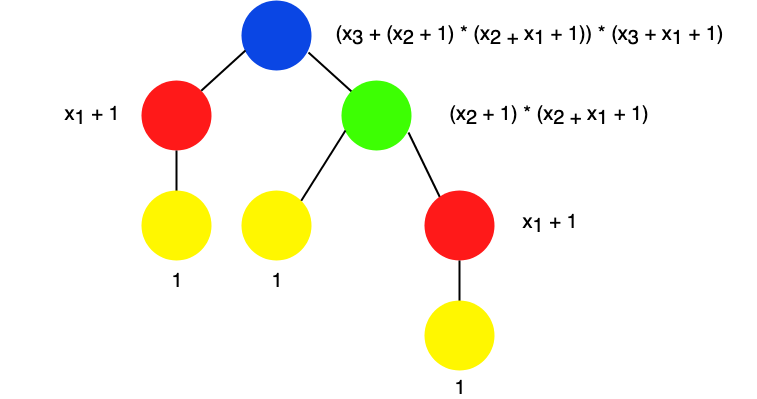
\includegraphics[width=8.5cm]{figuras/treeIsomorphism.png}
  \caption{Example of a tree with the hash of each node. }
\end{figure}


On the above picture we can see that the hash function is cumulative, and it forms a polynomial function in the end. The code for the above algorithm can be written as following in C++14:

\begin{lstlisting}
vector< vector<int> > adj; // Adjacency list of the graph
vector<long long> x; // X values for hash calculation
vector<int> d; // Height of each node
const int MOD = 1e9 + 7;
long long hashTree(int u, int p) {
   long long myHash = 1;
   for (int v : adj[u])
      if (v != p)
         myHash = (myHash * (d[h[u]] + hashTree(v, u))) % MOD;
   return myHash;
}
\end{lstlisting}

The hash of a tree can be defined recursively by the hashes of its subtrees. We can define the values of the array \( X \) as random values between \( 0 \) and \texttt{MOD - 1}. We can also trivially calculate the height of each node recursively. The algorithm described is linear.

One interesting caveat of this problem is that, although hashing trees to check for isomorphism only works with rooted trees, we can make it work for the problem of checking tree isomorphism for arbitrary trees. The basic idea is that we can root the tree by the center or centroid of tree (Because we know that we only have at most 2 centers or centroids on a tree). If we have more than one center or centroid, we can calculate the hash of the tree rooted by both and check if at least one of the hashed match. As this is not on the scope of this text I will limit the explanation here, but one can learn more about it in the bibliography \citep{Centroid}.

It is also important to cite here that there is another algorithm, the Aho-Hopcroft-Ulman algorithm, that runs in worst case linear time complexity that also solves the tree isomorphism problem. This algorithm is based on comparing both trees in a bottom up fashion \cite{AHU}.

SPOJ Problem: \url{https://www.spoj.com/problems/TREEISO}

%% May put there other applications such as consistent hashing 
\par

%% ------------------------------------------------------------------------- %%
\chapter{Final Remarks}
\label{cap:conclusions}

As we can see by previous chapters, hash functions and hash tables are very wide topics, with several details that we can have pages and pages with explanations. During this text the goal is to give a glance of how to implement a hash table data structure, with some other applications of the hash function itself.

It is important to notice that almost every programming language has it's implementation of a hash table, with some having a built-in implementation of a hash function for external usage. The most famous that we can cite here is Java, C++ (which have an implementation on STL), Golang, Python, Ruby, C\# and Scala. It's implementation may differ among paradigms as well, for example although in Scala Mutable hash maps uses chaining hashing, it also uses a Hash Trie for immutable hash maps, which is a complete different implementation with it's own specificalities and benefits for functional programming languages. \citep{hashMapAnalysis} 

One other interesting fact about hash tables is that it is an example about how memory locality is important in modern data structures. Memory locality is the proximity of the data accessed, which means that the data of your data structure is close to each other and it is ``cache friendly''. Although not accounted by usual complexity analysis, it is an important factor for regular used data structures, as one of the key performance factors of modern day processors.

During this text I also realized how deep we can go in each hash related topic. For that reason there are many contents that are not included here but are interesting to learn about. The main topics that would be included if I had more time were:

\begin{itemize}
\item Consistent Hashing
\item Distributed Hash Table
\item A deep analysis of the hash tables implemented during this text
\end{itemize}

Consistent hashing is a very interesting topic, because it is a special kind of hash function commonly used to implement sharded databases. It is special because when the table is resized, only \( \frac{K}{n} \) keys needs to be remapped on average, where K is the number of keys and N is the number of slots.\citep{wikiConsistent} This is very interesting and very useful in the context of databases because it easily allows horizontal scaling (that is, adding more machines).

Another interesting topic that I would have liked to discuss is distributed hash tables. A very used application in modern day, distributed hash table is a service that simulated a hash table lookup in a distributed environment. Common examples of this is modern services such as Memcached and Redis, that allow fast responses and scaling in modern web applications.

Lastly, it would be interesting to do a deep analysis of the hash tables implemented during this text. This would be different because we would see in practice many of the trade-offs discussed during this text, such as memory locality. There are many different factors in a deep analysis like this, like testing with different load factors, different deleting strategies, and different queries (random queries or queries closer to the 80/20 rule).

\par

%!TeX root=../tese.tex
%("dica" para o editor de texto: este arquivo é parte de um documento maior)
% para saber mais: https://tex.stackexchange.com/q/78101/183146

% Os capítulos de compõem a dissertação/tese, com numeração normal, podem
% ser inseridos diretamente aqui ou "puxados" de outros arquivos
%% ------------------------------------------------------------------------- %%
\chapter{Introduction}
\label{cap:Introduction}

One of the most used data structures in computer science are dictionaries, which are also known as associative array, map or symbol table. Those are a collection or key-value pairs, where all pairs have different keys, which support operations of adding a new pair, finding a pair given the key, and deleting a pair. If one thinks about it, this is perhaps one of the most executed tasks in many software systems. For instance, the call history of numbers on a cell phone shows for each phone number, the owner of that number. In a dictionary we can insert a phone number and its owner, so that given a phone number one can retrieve the owner. 


\begin{figure}[h!]
  \centering
  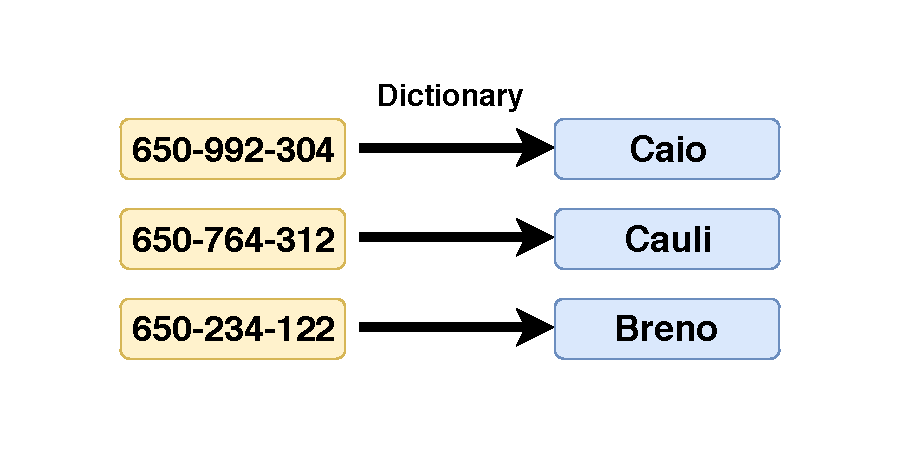
\includegraphics[width=12cm]{figuras/dictionary-example.pdf}
  \caption{Example of a dictionary that associates phone numbers to contact names. }
\end{figure}

Other use of a dictionary that we can think is to count the frequency that a certain number was called. One of the most used implementation of dictionaries is with a hash table. A key component in the implementation of a hash table is a hash function. This function usually takes the key of the key-value pair we want to add or update in the table and ``digest'' it into a number. That number is then used to identify the value, in this structure that we call hash table. In our example, the keys are phone numbers and the values are contact names.

An example of a hash function, that ``digest'' the phone numbers is the following: \\

\bigskip

\begin{figure}[h!]
  \centering
  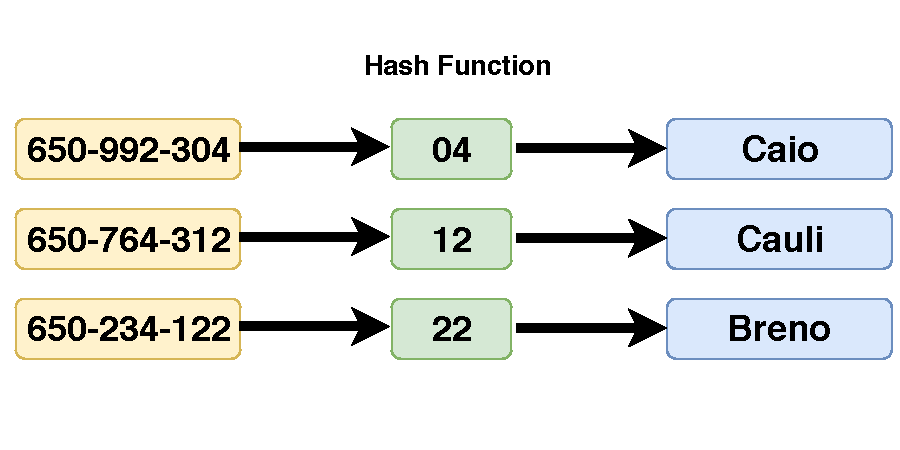
\includegraphics[width=12cm]{figuras/phone-hash-example.pdf}
  \caption{Example of a hash function hash function that just take the last 2 digits of the phone number }
\end{figure}

\medskip

As you can see this is a pretty simple function, it simply take the last 2 digits of each phone number. In this specific case, this is enough to uniquely identify each phone. We can imagine a function that can't uniquely identify each phone number, like getting just the last digit, in this case, Cauli's and Breno's numbers would have the same hash value, a collision in the table. Handling collisions in a hash table is a complete topic by itself, and it will be addressed in Chapter 3, Hash Tables. 

Handling collisions is actually a very important topic in hash tables and that is because the vast majority of hash functions will have collisions. To picture that we recall the ``Birthday Paradox'', that states that we only need 23 people in a room to have a chance greater than \( 50\% \) of 2 or more people having the same birthday. In Donald Knuth's famous book, The Art of Computer Programming (Vol. 3, Chapter 6.4) \citep{TAOCP3}, he uses as an example a function from a 31-element set to a 41-element set, and from about \( 10^{50} \) functions only about \( 10^{43} \) give distinct values for each argument, that is about 1 in every 10 million functions. This shows that we will have collisions more often than not, so knowing how to deal with it is a major problem that can not be neglected.

Hash functions and hash tables are among the most classic topics within computer science, yet is still one of the topics with most debate about what is state of the art. While the hash table was invented in 1953, widely discussed by Donald Knuth in his book, there are still many tweaks that can be made to boost its performance for specific use cases. One great example is F14, an open-source memory efficient hash table by Facebook \footnote{F14 is open sourced: \url{https://engineering.fb.com/developer-tools/f14/}}.

An example of lack of consensus in this area are the different hash functions and hash table implementations in different languages. There is no clear consensus on how to decide the size of a hash table, what are the trade-offs of the collision-resolution algorithms or even what defines a good hash function. Hopefully, we got years of research on the topic to study and present a view on the subject, and that is what I am presenting throughout this undergraduate thesis.

%% If you want it maybe interesting to cite Cassandra and other hash tables here.

\par

%% ------------------------------------------------------------------------- %%
\chapter{Hash Functions}
\label{cap:Hash Functions}

%% ------------------------------------------------------------------- %%
%\begin{itemize}
%\item Define Hash Function
%\item Give some examples of hash functions (Multiplicative / Remainder)
%\item Present Dragon Book metric and Evaluate hash functions
%\end{itemize}
%% ------------------------------------------------------------------- %%

Outside computer science, the word \textit{``hash''} in the English language means to ``chop'' or to ``mix'' something. This meaning is entirely related to what hash functions are supposed to do. Hash functions are functions that are used to map data of an arbitrary size to data of a fixed size \citep{HashFuncWiki}.

They have wide applications in computer science, being used in information and data security, compilers, distributed systems and hardcore algorithms. In this chapter we first define and explain the basics of a hash function, then we give an intuition in some metrics that tries to capture the idea of what is expected of a good hash function, as discussed in the famous \textit{``Red Dragon Book''} \citep{DragonBook} along with some reproduction of known results in the area.

The value extracted from the hash function for an object or key is usually called \textit{hash value} or simply \textit{value}. The hash value is in general, but not necessarily, smaller than the object that generated it. For example, we can have a hash function that takes Gigabytes or Terabytes files and return an 8 bytes hash value.

\begin{figure}[h!]
  \centering
  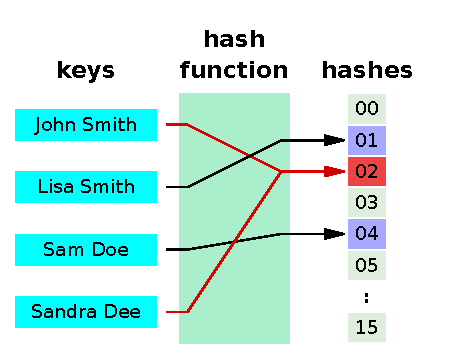
\includegraphics[width=6cm]{figuras/hash-function.pdf}
  \caption{Example of a hash function from string to 4 bit integer. Source: Wikipedia, Jorge Stolfi }
\end{figure}

\bigskip

\section{Definition}

A hash function over a set \( X \) a function \( H \) that takes an element \( x \) in \( X \) and associate to \( x \) a integer \( H(x) \) in the interval \( [0,M) \), for some integer \( M \). In symbols
\[ H: X \rightarrow [0, M) \]
When dealing with hash tables, \( X \) is the set of possible keys and \( M \) is the size of the table, which is usually just an array. Moreover, we saw earlier that hash functions are usually more useful when \( |X| > M \). This is the same definition used by Donald Knuth \citep{TAOCP3} and some articles \citep{RobinHoodHashing}. This definition makes sense for our purpose because we will be talking mostly about hash functions used in hash tables. In that case we want integers that will be indexes in an array (as we will see later on). In other cases we may see hash values as strings, like for when we hash an string for password storage or when we use a hash function in files for checking integrity (for when we are checking if two files are the same). For the goal of this thesis we will not be focusing on those functions, but it is important to notice that strings can also be easily associated to integers if we just look at their bytes.

For our purpose we are looking for a hash function that performs well for the construction of hash tables. Ideally, these functions should be fast to compute and minimizes the number of collisions. Depending on our goals we might want a different metric, for check-sums for example we may want a function that is very sensible to changes, and for passwords one that is very hard to find its inverse, those are so called cryptographic functions. For some collision resolution techniques, as we will see later, we may also want that the hash function disperse the values well too. Intuitively, a hash function should look like a random function having a given key as seed.

As written in Knuth's book, we know that it is theoretically impossible to create a hash function that generates true random data from non random data in actual file, but we can do pretty close to that or in some cases, even fewer collision than an uniformly random function. Knuth describes two specific methods for simple hash function, named \textit{division hashing} and \textit{multiplicative hashing} techniques. As the name suggests, the first is based on division operation and the former on multiplication operation.

\section{Division and Multiplicative Methods}

The \textit{division hashing} method maps an integer \( X \) associated to the data to its remainder modulo an integer \( M \). Supposing that we can represent the data as a non negative integer \( X \) the division hashing would be to choose a value M and the hashing function would be \( X \mod M \). The code would look as following:

\begin{lstlisting}
unsigned int divisionHashing(unsigned int X, unsigned int M) {
  return X % M;
}
\end{lstlisting}

A good hash function combines number theory, statistics and engineering and in general, large prime numbers tend to be a good value to \( M \), to avoid unwanted patterns or repetitions. One great example of this is if \( M \) is even, then the parity of hash value of \( X \) will match the parity of \( X \) (which will cause a bad distribution). The same pattern will happen in different intervals for different powers of \( 2 \).

For \textit{multiplicative hashing}, let's first suppose once more that we can represent the data as a non-negative integer \( X \) and we have chosen a constant \( S \), where \( 0 < S < 1 \). Then we multiply \( X \) by \( S \) and extract the fractional part of \( X \times S \), that is \( X \times S \mod  1 \). We can calculate that by doing: \( X \times S - \lfloor X \times S \rfloor \). Then we multiply that value, that will be between 0 and 1, by \( M \). The code of what was described above would look as following:

\medskip

\begin{lstlisting}
unsigned int multiplicativeHashing(unsigned int X,
                                   double S,
                                   unsigned int M) {
  double alpha = (double) X * S - floor((double) X * S);
  return (unsigned int) floor(alpha * (double) M);
}
\end{lstlisting}

In Knuth's book he describes \( S \) as being an integer \( A \) divided by \( w \), where \( w \) is the size of a ``word'' in our computer. He restricts \( A \) to be relatively prime to \( w \). That definition is often useful if you want to retrieve a value \( Y \) for a given hash value \( F \). This can be done via Bezout theorem \citep{TAOCP3}. It is good to note here that if \( H(X) = F \) and \( H(Y) = F \), \( X \) is not necessarily equal to \( Y \), as two different keys can have the same hash value.

\section{Hashing Strings}

We have many ways of converting non numerical data to non negative integers. In the end, it is all just a sequence bytes, that when read in a specific way form another type of data, such as images or strings. For example, one way of transforming a string to a non-negative integer is summing the ASCII value of its characters. The C++14 code for that would look as following:

\begin{lstlisting}
unsigned int stringToInteger(string str) {
  unsigned int hashValue = 0;
  for (char c : str) {
    hashValue += (int) c;
  }
  return hashValue;
}
\end{lstlisting}

We always use unsigned integers for our non negative integer calculations due to the natural modulo operation of it on overflow cases. It is equivalent to having a \( \mod \ 2^{32} \) every time it overflows, as we only look at the leading 32 bits. We can also use XOR function to mix numbers together. 

There is also a very common type of hash functions that tend to work pretty well for strings \citep{DragonHashFunc}. It is a ``superset'' of multiplicative hash functions, or a generalization. The C++14 code would look as following:

\begin{lstlisting}
unsigned int hashForString(string str,
                           unsigned int initialValue,
                           unsigned int multiplier,
                           unsigned int modulo) {
  unsigned int hash = initialValue;
  for (char c : str) {
    hash = (multiplier * hash + (int)c);
  }
  return hash % modulo;
}
\end{lstlisting}

The above function is very common for string hashing, and by just choosing a different initial value and multiplier we can have completely different hash functions. Although using summing or using XOR to combine the previous hash value with the new character usually don't provide much difference, with XOR operation we do not need to worry about overflow. Some values are of known hash functions, for example with \texttt{multiplier = 33} and \texttt{initialValue = 5381} generates \textit{Bernstein hash djb2} \citep{BernsteinHash} or \texttt{multiplier = 31} and \texttt{initialValue = 0} generates \textit{Kernighan and Ritchie's hash} \citep{KernighanHash}. Those are famous functions and their values are not chosen randomly, as there are some factors that maximizes the chance of producing a good hash function, where good means low collision rate and fast computation. Those factors are:

\begin{itemize}
\item The multiplier should be bigger than the size of the alphabet, in our case usually 26 for English words or 256 for ASCII. That is the case because if it is smaller we can have wrong matches easier. For example, suppose that \texttt{multiplier = 10} and \texttt{initialValue = 0}, we have \( H('ABA') = H('AAK') = 7225 \) before taking the modulo operation.

\item The multiplication by the multiplier should be easy to compute with simple operations, such as bitwise operations and adding. That is quite intuitive as we want a hash function that is fast to calculate. 

\item The multiplier should be coprime with the modulo. That is because if not we will ``cycle'' hashes at a greater rate than the modulo (We can use some modular arithmetic to prove that). Usually prime numbers tend to be good multipliers.
\end{itemize}

\section{Quality of a Hash Functions}

Now that we know some good templates for producing hash functions lets try to find a concrete metric or formula that measures the quality of a hash function. Fortunately, the famous book Compilers: Principles, Techniques, and Tools, also known as ``Red Dragon Book'' \citep{DragonBook}, has already proposed a quantity to measure the quality of a hash function. The formula gives this quantity:
\[ \mathlarger{\sum}_{j = 0}^{m - 1} \frac{b_j(b_j + 1)/2}{ (n/2m)(n + 2m - 1) }, \]
where \( n \) is the number of keys, \( m \) is the number of total slots and \( b_j \) is the number of keys in the \( j \)-th slot. The intuition for the numerator is that it represents the number of operations we will need to perform to find each element of the table. For example, we need 1 operation to find the first element, 2 to find the second, and so on. That means that we will end up with an arithmetic progression. We know that a hash function that distributes the keys according to an uniformly random distribution has expected bucket size of \( n / m \), so we can calculate that the expected value of the numerator formula is \( (n/2m)(n + 2m - 1) \). So that gives us a ratio of collisions (thinking just about operations to access a value) of ``our'' hash function with an ``ideal'' function. That means that a value close to \( 1.00 \) of the above formula is good, and values below to \( 1.00 \) means that we had less conflicts than an uniformly distributed random function.

From common data as used in Dragon Book and Strchr website \citep{DragonHashFunc} I will reproduce some tests with the previously cited hash functions.

\begin{figure}[h!]
  \centering
  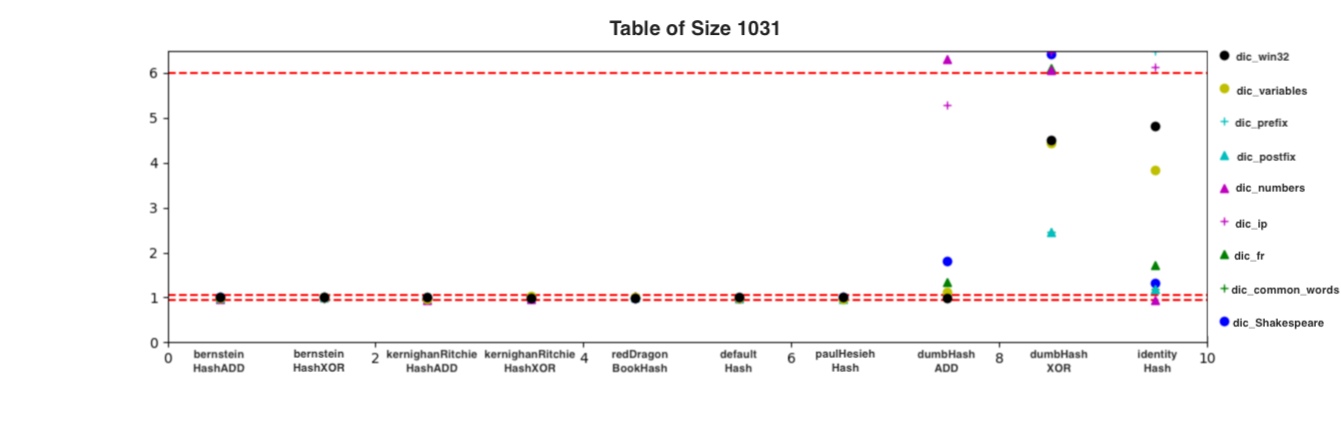
\includegraphics[width=14cm]{figuras/1031HashFunc.png}
  \caption{Functions tested against a ``small'' table}
\end{figure}

\medskip

\begin{figure}[h!]
  \centering
  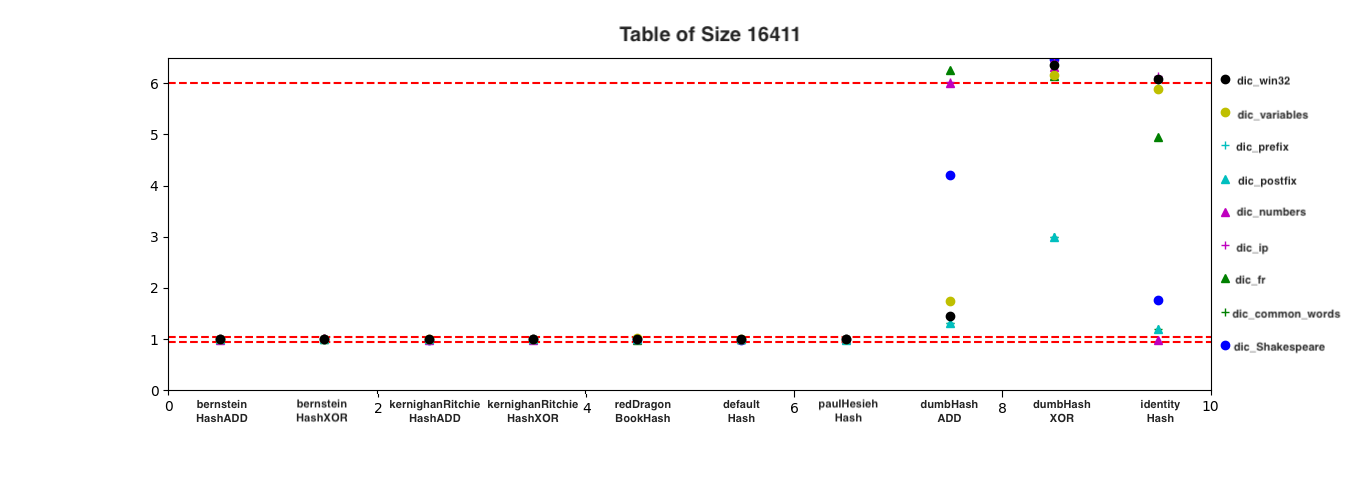
\includegraphics[width=14cm]{figuras/16411HashFunc.png}
  \caption{Functions tested against a ``medium'' sized table}
\end{figure}

\medskip

\begin{figure}[h!]
  \centering
  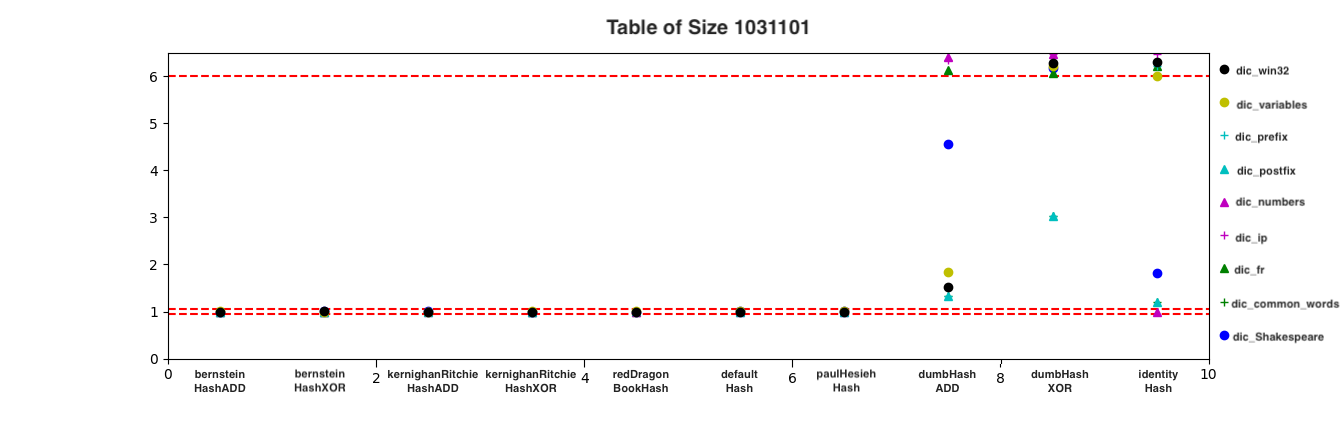
\includegraphics[width=14cm]{figuras/1031101HashFunc.png}
  \caption{Functions tested against a ``large'' table}
\end{figure}

\medskip

The results are shown in the same way displayed in the Red Dragon Book, with hash functions in the \( x \) axis and the ratio displayed in the \( y \) axis, with different identification for each file. We consider three sizes of tables to to count collisions, a ``small'', ``medium'' and a ``large'' table, the small table having a load factor (The percentage of the table occupied) of approximately \( \sim 0.5 \), the medium with \( \sim 0.05 \) and large with \( \sim 0.005 \). It's assumed that the modulo is not the responsibility of the hash function, so all hash functions return values from 0 to \( 2^{32} - 1 \), and the modulo is taken depending on the size of the table. From that we can already see that the load factor doesn't make a good hash function bad, but expose problems of ``bad'' hash functions in some cases. 

Another fact that it is important to notice from the graph is the red dotted lines. The top one is the ``Upper'' threshold, which results greater than 6 are just considered ``Big'', as in some cases the ratio exploded to values up to 200. The lower 2 red lines are in \( y = 1.05 \) and \( y = 0.95 \) which is the interval that we consider a hash function to have ``Good'' values. 

The tests were made with 10 different hash functions, tested against 9 different files (Provided by strchr website). All of the code used to test this can be found in the github repo \citep{GithubRepo}. The 10 hash functions are the following:

\begin{itemize}
\item \textbf{bernsteinHashADD}: The Bernstein hash function described earlier. We use the given hash template adding the elements. The multiplier is 33 and initial value is 5381. In the end we XOR the bits of the hash with itself shifted 16 to the right (That is half of the bits with our implementation).
  
\item \textbf{bernsteinHashXOR}: The same as above but substituting the first adding operator by the XOR operation.

\item \textbf{kernighanRitchieHashADD} The Kernighan and Ritchie Hash function described earlier. We use the given hash template adding the elements. The multiplier is 31 and initial value is 0.

\item \textbf{kernighanRitchieHashXOR} The same as above but substituting the first adding operator by the XOR operation.

\item \textbf{redDragonBookHash} The hash function tested in the Red Dragon Book. It is described as x65599 in the book.

\item \textbf{defaultHash} The default hash function of C++ standard template library.

\item \textbf{paulHesiehHash} A fast hash function described by Paul Hesieh. It is fast to calculate and more complex than Knuth multiplicative or division Hashing.
  
\item \textbf{dumbHashADD} A hash function that simply add all characters.

\item \textbf{dumbHashXOR} A hash function that simply XOR all characters.

\item \textbf{identityHash} A hash function that takes the first 4 bytes of the string.  
\end{itemize}

We have a variety of hash functions, with all being considered ``fast'' hash functions. The files tested include common words in English and french, strings of some IP values, numbers, common variable names and words with common prefix and suffix.

First thing we can notice from those graphs is that changing the ADD function to XOR doesn't make a good multiplicative hash function bad. Both are actually ``Equivalent'' given that we are also multiplying the values. For \texttt{dumbHashADD} and \texttt{dumbHashXOR} we can see clear differences, with \texttt{dumbHashXOR} being clearly worse. This can be explained by the cancellation property of XOR. We can see this example on the hash of this IP below:

\texttt{dumbHashXOR('168.1.1.0') = dumbHashXOR('168.2.2.0') = dumbHashXOR('124.6.8.0')}

We can see that many different IPs have the same hash value. More than that, XOR don't increase the number of bits, so all the hashes will be of just 1 byte.

Other thing that we can notice is that ``identity'' hash is good or perfect in some cases. One obvious case that ``identity'' function works perfectly is for numbers as we will have 0 collisions. Some languages, like Python 3, use the identity function to calculate hash for integers, as it is very fast and produces no collisions. But we can see that for other cases, such as common prefix, it works terrible as we just get the first 4 bytes.

The most common multiplicative hash functions tend to work similarly well, being reasonably close to an uniformly random function (that is our ``ideal'' hash function) in all cases.

As we can see, we don't need a lot of complexity to make a good hash function for a hash table. We have some functions working better for some specific case, like identity function working well for numbers, but general functions already work well enough.

One thing that is important to note here is that hash function is a very vast topic, and here we just covered hash functions related to hash tables. Hash functions have applications in distributed systems (consistent hashing), database indexing, caching, compilers (Red Dragon Book) and cryptography. Each application has different requirements and make some hash functions better than others.
\par


%% ------------------------------------------------------------------------- %%
\chapter{Hash Tables}
\label{cap:Hash Tables}

%% ------------------------------------------------------------------- %%
%\begin{itemize}
%\item Define hash table and its operations
%\item Open Addressing Strategies (Linear Probing, Quadratic Probing, ...)
%\item Chaining Strategy (Simple Chaining, Move-to-front ...)
%\item Load factor and resizing/rehashing the table
%\end{itemize}
%% ------------------------------------------------------------------- %%


Hash tables or hash maps is one of the most used applications of hash functions. It is actually so used in computer science that is almost impossible to talk about one without mentioning the other. This data structure consists in associating a \textit{key} to a \textit{value} in a table. That is, given a \textit{key}, it can retrieve the  \textit{value} for it.

It is one of the possible, and many times considered the best, implementations of a dictionary. It has to implement the \texttt{insert}, \texttt{find} and \texttt{remove} operations, that can be accessed from outside the dictionary. It usually implements a lot of other private methods. 

This data structure is usually considered very useful among software engineers and computer scientists, although it usually has a linear worst case cost for retrieving, inserting and deleting a key-value pair. That is because hash tables usually have a constant average cost for those operations.

Moreover, when talking about hash tables we have the problem of key collision, that is when two keys map to the same hash value. As we saw in the previous chapter, collisions are more common than not, so collision resolution is a critical problem. To solve that problem, we have several techniques that involve different trade-offs. Those techniques are usually divided into two main categories, open addressing and separate chaining. Other problem to consider regarding this data structure is when to resize the hash table, to minimize the chance of collision and the use o memory. For this last one we usually consider a load factor, \( \alpha \), that is the ratio of keys with the available slots in the table.

\newpage

Also, hash tables can be easily abstracted to hash sets, commonly used to store a set of elements and check whether an element is in the set. We can abstract hash sets to a hash table always with an empty value. Hash sets are one of the common ways to implement sets in programming languages, like unordered\_set from C++14.

It is also important to notice that hash tables have applications in different areas of computer science also, like compilers, caches and database indexing.


\begin{figure}[h!]
  \centering
  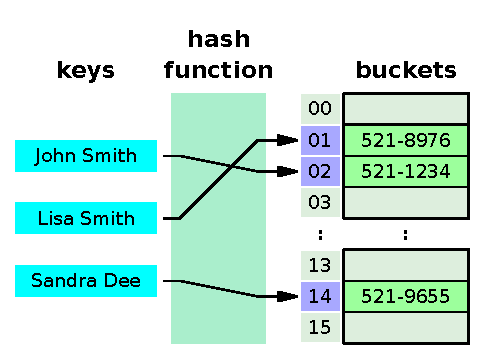
\includegraphics[width=12cm]{figuras/hash-table.pdf}
  \caption{Example of a hash table from string to string, more specifically name to phone number. Source: Wikipedia, Jorge Stolfi }
  \label{fig:hashTable}
\end{figure}

In the above figure (\ref{fig:hashTable}), we can see an example of a hash function that matches names of people to phone numbers, as we saw in the first chapter. This table has no collisions, and we can see that, for example, ``Jhon Smith'' has a hash value of 2 and his value in the table is ``521-1234''. That is we associated a names with phone numbers.

\newpage

\section{No collision open addressing hash table }

To start let's give an example of a hash table that has a perfect hash function, that is a function from \( X \) to \( [0, M) \) with no collisions from the used keys. For that example we use open addressing, that basically means that all data will be contained in an array (that is, the whole table). The operations \texttt{insert}, \texttt{find} and \texttt{remove} would be very easy to implement. For the sake of simplicity, we will assume all the keys are strings and values are integers. To start lets look at this simple class with dummy methods:

\begin{lstlisting}
class HashTable {
   vector< pair<string, int> > table;
   int m, n;
   
   HashTable() {
      m = 16;
      table.resize(m);
      n = 0;
   }

   unsigned int hashFunction(string s) {}
   
   void insert(string key, int value) {}

   int find(string key) {}

   void remove(string key) {}

private:
   double alpha = 1;
   void resizeIfNecessary() {}
}
\end{lstlisting}

As we can see it is pretty simple. The constructor builds a table of size \( 16 \), and we can assume a dynamic resizing every time the table is full. Later on we will see that this means that we resize every time the load factor, \( \alpha \), is equal to \( 1.00 \). We also can note that at the table part we are storing a pair of key and value, not just value. This is because we may want to retrieve all pairs of the table (like in a regular dictionary). The pairs are usually unordered (If they are not ordered by chance \dots). Actually, if one needs the set of keys sorted by total order, very likely hash tables are not the appropriate data structure. We will skip the implementation of hashFunction, as we already saw plenty of it in the last chapter, so we will go right in for the implementation of \texttt{insert}:

\begin{lstlisting}
void insert(string key, int value) {
  resizeIfNecessary();
  unsigned int idx = hashFunction(key);
  table[idx] = pair<string, int>(key, value);
  n++;
}
\end{lstlisting}

That is pretty simple, that is mostly because we will assume that we will never have a collision, so we just put the key on the position returned by the hash function. The method \texttt{find} is implemented as following:

\begin{lstlisting}
int find(string key) {
  unsigned int idx = hashFunction(key);
  if (table[idx].first == key)
    return table[idx].second;
  return 0;
}
\end{lstlisting}

Also very simple, we always know the value will be in position returned by idx. The \texttt{remove} will be of the same simplicity, as following:

\begin{lstlisting}
void remove(string key) {
  unsigned int idx = hashFunction(key);
  table[idx].first = pair<string, int>("", 0);
  n--;
}
\end{lstlisting}

Here we make the assumption that an empty position has an empty string. We could also carry a boolean, usually called a tombstone, to check if the position is occupied or not. If the hash function is perfect, than the insert, find and delete operations can be performed in constant time and linear space.

\section{Open addressing}

We can define open addressing in a general way as a hash table algorithm where the data always stay within the same vector. So, in the case of a collision, we need to define a systematic way to traverse the table. The sequence of elements we need to traverse when we have a collision is called \textit{``Probe sequence''}. With that our hash function would change to the following:
\[ h(x, i) \],
where \( x \) is our key and \( i \) is the probe sequence number. So every time we have a collision in \( h(x, i) \) we can simply go to \( h(x, i + 1) \). Given that, lets look into some different probe sequences.

\section{Linear Probing}

Linear probing is one of the most simple an practical probe sequences known. The probe sequence is basically:
\[ h(x, i) = (H(x) + i) ~\mathrm{mod}~ M \],
where \( M \) is the table size. That is a very simple probe sequence with not much secret on it. To implement the \texttt{insert} we can do the following:

\begin{lstlisting}
void insert(string key, int value) {
  resizeIfNecessary();
  unsigned int idx = hashFunction(key);
  while (table[idx] != pair<string, int>("", 0))
    idx = (idx + 1) % m;      
  table[idx] = pair<string, int>(key, value);
  n++;
}
\end{lstlisting}

That assumes that \texttt{pair<string, int>("", 0)} is the empty position, and performs a linear search until it finds one empty position to put the new (key, value) pair. The implementation of \texttt{find} is very similar:

\newpage

\begin{lstlisting}
int find(string key) {
  unsigned int idx = hashFunction(key);
  while (table[idx] != pair<string, int>("", 0)) {
    if (table[idx].first == key) 
      return table[idx].second;
    idx = (idx + 1) % m;
  }
  return 0; // Default value
}
\end{lstlisting}

It performs a linear search until it finds the element. If the key is not found the function returns a default value, that in our case is 0. 

For removal, we have the problem that we cannot leave ``holes'' in our table. That will be discussed more in depth later on the section ``How to delete an entry''. For now we will remove the element, and reinsert the key-value pairs that come right after it:

\begin{lstlisting}
void remove(string key) {
  unsigned int idx = hashFunction(key);
  while (table[idx] != pair<string, int>("", 0)) {
    if (table[idx].first == key) 
      break;
      idx = (idx + 1) % m;
  }
    
  if (table[idx].first == key) {
    table[idx] = pair<string, int>("", 0);
    vector< pair<string, int> > toRehash;
    int j = (idx + 1) % m;
    while (table[j] != pair<string, int>("", 0)) {
      toRehash.push_back(table[j]);
      table[j] = pair<string, int>("", 0);
      j = (j + 1) % m;
    }
    for (auto p : toRehash) {
      insert(p.first, p.second);
    }
    n--;
  }  
}
\end{lstlisting}

With that, the three operations have linear time complexity in the worst case. As we saw, we know hash functions that are considered good, with a rate of collision very close to an uniformly random function. Those functions will leave us with an expected constant time complexity for those operations, and we will see later on that in practice it is much faster than linear access. Another great benefit that linear probing has, specially when compared to other collision resolution strategies, is locality and cache friendliness.

However linear probing has the problem of clustering, that is long chains of occupied positions. This generates a greater problem, as long chains are only expected to get longer and longer. This can get worse if the hash function is not too sensitive to changes, having a lot of sequential hash values. 

\section{Quadratic Probing}

Another strategy for resolving collisions is quadratic probing. In this case, the probe sequence can be defined as:
\[ h(x, i) = (H(x) + i^2) \mod M \]
That solves the problem of having sequential hash values. The implementation of quadratic probing is very similar to the implementation of linear probing, with the exception that instead of adding one for each step we can keep the initial value and add the square of a counter.

However, quadratic probing doesn't solve the problem of clustering. Long chains are still expected to get longer and longer, the only difference is that the positions that lead to a longer chain are better distributed in the table. Another thing to notice is that quadratic probing has a worse locality and cache friendliness than linear probing. 

\section{Double Hashing}

As we saw the two strategies above have the problem of clustering, due to the fact that the sequences are the same for all keys. For that reason double hashing is a very good approach for open addressing. Double hashing probe sequence can be defined as following:
\[ h(x, i) = (H_1(x) + i * H_2(x)) \mod M \],
where \( H_1 \) and \( H_2 \) are two distinct hash functions. In that way not only the initial hash value will depend on \( x \), but it's probe sequence offset (that is, the number of slots between \(h(x, i) \) and \(h(x, i + 1) \)) will too. The implementation of double hashing is very similar to both quadratic and linear probing, except that we sum a different offset.

These last three implementations of hash table give us linear time worst case complexity for all operations and constant time expected time complexity under the simple uniform hashing assumption.

\section{Robin Hood Hashing}

Robin Hood Hashing is an optimization technique regarding collision resolution with open addressing. It should be paired with Linear Probing, Quadratic Probing or Double Hashing, but usually it is paired with linear probing due to it is good locality and cache friendliness. It is basic is that it minimizes the distance of each key from its ``home Slot'', that is, its initial hash value position. \citep{RobinHoodHashing}. Also, Robin Hood hashing is one of the few open addressing strategies to be built-in in hash tables of some languages, such as Rust.

In order to minimize the distance from each key from its home slot, Robin Hood hashing uses a concept that is called Probe Sequence Length, or PSL, of a key-value pair. The PSL of a key-value pair is the number of probes required to find that pair. For that reason we need to define a new class to store in our table, that we will call \texttt{Node}:

\begin{lstlisting}
class Node {
public:
   string key;
   int value;
   unsigned int PSL;   
   Node(string K = "", int V = 0, unsigned int P = 0):
      key(K), value(V), PSL(P) {}

   bool operator == (const Node& ot) {
      return key == ot.key && value == ot.value && PSL == ot.PSL;
   }
   bool operator != (const Node& ot) {
      return key != ot.key || value != ot.value || PSL != ot.PSL;
   }
};

const Node defaultNode = Node();
\end{lstlisting}

\texttt{Node} is a very simple class that stores a key, a value and an unsigned integer that is the PSL. The main idea around Robin Hood hashing it to move the Nodes with a low PSL in favor of Nodes with a high PSL. We can think of Nodes with a high PSL as poor, because we take longer to find it, and Nodes with a low PSL as rich because we can find them faster. For that reason the algorithm is called Robin Hood Hashing \citep{RobinHoodHashing}.

As explained when inserting an element we first look for an empty position. While searching for it, we check whether the \texttt{Node} that is in the way has a lower PSL than the Node that we are inserting, and if that is the case we swap them, securing a position for the current Node and move the other node forward. The implementation of this algorithm using Linear Probing would be the following:

\begin{lstlisting}
void insert(string key, int value) {
  resizeIfNecessary();
  unsigned int idx = hashFunction(key);
  Node toInsert = Node(key, value, 0);
  while (table[idx] != defaultNode) {
    if (toInsert.PSL > table[idx].PSL)
      swap(toInsert, table[idx]);         
    idx = (idx + 1) % m;
    toInsert.PSL++;
  }
  table[idx] = toInsert;
  n++;
}
\end{lstlisting}

For the \texttt{find} method we can use different lookup techniques. Here we will focus on the lookup that is most similar with linear probing, but with a tweak that will make finding that keys are not present faster. While searching for a key, we can calculate what the PSL of that key would be if were inserted, and if we find a Node with a greater PSL that means the pair is not present. That is because all Nodes after it will also have a PSL greater than the current PSL. The implementation of what was described above would be the following:

\newpage

\begin{lstlisting}
int find(string key) {
  unsigned int idx = hashFunction(key);
  unsigned int curPSL = 0;
  while (table[idx] != defaultNode) {
    if (table[idx].key == key) 
      return table[idx].value;
    // If the key were inserted it would be before this Node.
    if (table[idx].PSL > curPSL)
      break; 
    idx = (idx + 1) % m;
    curPSL++;
  }
  return 0; // Default value
}
\end{lstlisting}

For the removal we can apply \textit{backward shifting}. Although this will be discussed more in depth in the ``How to delete an entry'' section, this approach is unique to robin hood hashing and has a better performance than rehashing.

\textit{Backward shifting} consists in first clearing out the slot that contains the key to be removed, then shifting the following keys one step back until a Node with 0 PSL or an empty slot is encountered. The code for that would be the following:

\begin{lstlisting}
void remove(string key) {
  unsigned int idx = hashFunction(key);
  while (table[idx] != defaultNode) {
    if (table[idx].key == key) 
      break;
    idx = (idx + 1) % m;
  }
  if (table[idx].key == key) {
    table[idx] = defaultNode;
    while (table[(idx + 1) % m] != defaultNode &&
           table[(idx + 1) % m].PSL != 0) {
      swap(table[idx], table[(idx + 1) % m]);
      table[idx].PSL--;
      idx = (idx + 1) % m;
    }
    n--;
  }
}
\end{lstlisting}

We can always do that because the keys are always sorted according to the their home slot (That is, the first Node with PSL that is 0 that comes before them).

The worst time complexity of all operations is linear and the expected time complexity is constant. The expected length of the longest PSL in a full table is \( \log n \).
\section{Cuckoo Hashing}

Another well known strategy for collision resolution in open addressing is Cuckoo Hashing. It is a different strategy regarding the previous ones because it uses more than one array, usually two, but up to any number of arrays, to perform collision resolution. It is usually classified as open addressing because each slot can hold up to one key-value pair. For this explanation let's assume that we are using two arrays. Cuckoo hashing requires also one hash function per array used, in our case two hash functions.

%% Image representing cuckoo hashing

For the insertion of cuckoo hashing we try to insert the key in the first table and if a collision occurs we swap the key value pair that we are trying to insert with the element that is currently on the table and then try to insert it on the next array. If a collision occurs in the other array we swap the pairs and try again on the next one, until we find an empty position or we reach a certain threshold. The threshold is important because we can have cycles.

%% Image Representing insertion.

The code for the algorithm described above is the following:

\begin{lstlisting}
void insert(string key, int value) {
  resizeIfNecessary();
  unsigned int j = 0, it = 0;
  unsigned int idx = hashFunction(key, j), lim = maxLoop();
  pair<string, int> toInsert = pair<string, int>(key, value);
  while (table[j][idx] != pair<string, int>("", 0) && it < lim) {
    swap(table[j][idx], toInsert);
    j = (j + 1) % numTables;
    idx = hashFunction(toInsert.first, j);
    it++;
  }
  if (it == lim)
    resize();
  table[j][idx] = toInsert;
  n++;
}
\end{lstlisting}

This gives a very strong property to this collision resolution approach, that is every key value pair will be in its corresponding position in exactly one of the arrays. And this will give constant Lookup and Removal time. 

In order to find a key value pair we just need to look if the key value pair is present in one of the tables. The code is the following:

\begin{lstlisting}
int find(string key) {
  for (unsigned int j = 0; j < numTables; j++) {
    unsigned int idx = hashFunction(key, j);
    if (table[j][idx].first == key)
      return table[j][idx].second;
  }
  return 0;
}
\end{lstlisting}

For removal we can simply erase the key value pair from the table, as no key value pair affect the lookup of any other pair. The code is the following:

\begin{lstlisting}
void remove(string key) {
  for (unsigned int j = 0; j < numTables; j++) {
    unsigned int idx = hashFunction(key, j);
    if (table[j][idx].first == key) {
      table[j][idx] = pair<string, int>("", 0);
      n--;
    }
  }
}
\end{lstlisting}

Besides the amazing property of guaranteed constant lookup and removal, Cuckoo hashing has the problem of cycles during insertion, which can cause unwanted rehashes. To deal with that, many implementations also use a stash to keep a constant amount of elements in case the threshold is reached. A stash is a sort of ``bin'' of fixed size that we put key-value pairs that failed insertion, and during lookup we would also need to look at the stash.

\section{Coalesced Hashing}

Another well known strategy, described in Donald Knuth book \citep{TAOCP3}, is Coalesced Hashing. Although without much advantages in contrast with previous strategies, coalesced hashing condenses the hash table well in memory and is very similar to Chaining Hashing, our next topic.

The main idea of coalesced hashing is to add a new parameter to our key value pairs in the table, called next. That would create linked lists in the table in case we have a collision. To find the next element in case a collision we can find the first free bucket looking to the array in reverse order. The function to find the next free bucket is the following:

\begin{lstlisting}
int nextFreeBucket() {
  for (int i = m - 1; i >= 0; i--) {
    if (table[i].isDefaultNode())
      return (unsigned int)i;
    }
  return -1; // error
}
\end{lstlisting}

To insert an element, in case of a collision, we need to traverse the linked list beginning on the bucket that the key hashes to until the end. Then we add a new Node to the end of the linked list, pointing to the next free bucket. The complete code of the insertion algorithm will be shown later on.

To lookup for an element, we can traverse the linked list until we find a matching Node. The code for the find method would be the following:

\begin{lstlisting}
int find(string key) {
  unsigned int idx = hashFunction(key);
  while (idx != -1) {
    if (table[idx].key == key) 
      return table[idx].value;
    idx = table[idx].next;         
  }    
  return 0;
}
\end{lstlisting}

Removing a node in coalesced hashing is very difficult, as many other nodes can depend on it. For this reason the best way to delete an element in coalesced hashing is by using a strategy that is known as tombstoning. The idea of this strategy is to put a placeholder value, that will be considered as occupied by the find method but as free by the insertion method. The code for that would be the following:

\begin{lstlisting}
void remove(string key) {
  unsigned int idx = hashFunction(key);
  while (idx != -1) {
    if (table[idx].key == key) 
      break;
    idx = table[idx].next;         
  }
  if (table[idx].key == key) {
    table[idx].transformTombstone();
    n--;
  }
}
\end{lstlisting}

For this reason, the insertion method explained earlier on would have to be a little bit different, considering tombstones. The code would look like the following:

\begin{lstlisting}
void insert(string key, int value) {
  resizeIfNecessary();
  unsigned int idx = hashFunction(key);
  Node toInsert = Node(key, value, -1);
  if (!table[idx].isDefaultNode()) {
    while (table[idx].next != -1 && !table[idx].isTombstone())
      idx = table[idx].next; 
    if (!table[idx].isTombstone()) {
      table[idx].next = nextFreeBucket();
      idx = table[idx].next;
    }
  }
  table[idx] = toInsert;
  n++;
}
\end{lstlisting}

\section{Chaining hashing}

Chaining hashing, also known as closed addressing, is the implementation of a hash table using a container, usually called bucket, to store the (key, value) pairs with a given hash. On this implementation, each bucket of the table is a linked list, that will carry the key value pair in our case. We deal with collisions with this implementation by adding a new node to the start of the list.

This implementation is considered simpler than open addressing, usually because the way of dealing with collisions is clearer. Also it is less system dependent if we consider performance (as we saw one of the key advantages of open addressing is that it is cache friendly). That is one of the key reasons that C++ uses chaining hashing for its default implementation of unordered\_hash \citep{HashTableProposal}.

Below we will discuss an implementation of chaining hashing.

\section{Simple Chaining Hashing Algorithm}

For this chaining hashing implementation we will use C++14 STL data structure list as our container. list is a doubly linked list. For our \texttt{insert} we can implement it in the following way:

\begin{lstlisting}
void insert(string key, int value) {
  resizeIfNecessary();
  unsigned int idx = hashFunction(key);      
  table[idx].emplace_front(key, value);
  n++;
}
\end{lstlisting}

As we can see it is a very simple implementation, we just push a new element in the front of the list pointed in the idx. As before we add the counter of elements in the list and call resizeIfNcessary().

For \texttt{find} we can implement in the following way:

\begin{lstlisting}
int find(string key) {
  unsigned int idx = hashFunction(key);
  auto it = find_if(table[idx].begin(), table[idx].end(),
                    [&key](auto& kv) { return kv.first == key; });
  if (it != table[idx].end())
    return it->second;
  return 0;
}
\end{lstlisting}

That implementation is very succinct but uses some of the features of C++14 (such as generic lambdas). For \texttt{erase} we can implement in a very similar fashion:

\begin{lstlisting}
void remove(string key) {
  unsigned int idx = hashFunction(key);
  auto it = find_if(table[idx].begin(), table[idx].end(),
                    [&key](auto& kv) { return kv.first == key; });
  if (it != table[idx].end()) {
    table[idx].erase(it);
    n--;
  }
}
\end{lstlisting}

As we can see, with linked list it is clearly easier to erase an element. 

The naive algorithm of chaining hashing with a linked list gives linear worst time complexity for all operations and constant expected time complexity under the assumption of simple uniform hashing. 

% THINK ABOUT PUTTING THAT.

%One interesting thing to notice regarding chaining hashing implementation in C++ is that we may have a greater performance with implementations using vector instead of list, because of the better locality of vector.

\section{Move to front}

One great optimization to chaining hashing is every time you execute the \texttt{find} method to move to the beginning of the container the element that was found. That will keep in the beginning of the container the elements that are searched the most. As in many applications we can apply the 80 / 20 rule this greatly helps in time performance. The 80 / 20 rule is basically the idea that usually, 20\% of the keys will represent 80\% of the searches, this rule is also cited by Knuth \citep{TAOCP3}.

If our container is a linked list we can easily adapt the above implementation to move to front every time we search an element, with const time complexity cost. The implementation of \texttt{find} would be the following:

\begin{lstlisting}
int find(string key) {
  unsigned int idx = hashFunction(key);
  auto it = find_if(table[idx].begin(), table[idx].end(),
                    [&key](auto& kv) { return kv.first == key; });
  if (it != table[idx].end()) {
    if (it != table[idx].begin()) {
      table[idx].splice(table[idx].begin(), table[idx],
                        it, next(it));
    }
    return it->second;
  }
  return 0;
}
\end{lstlisting}

Here we are using the \texttt{splice} method of list C++ standard library to move an element inside a list. This still keeps the complexity of \texttt{find} in linear worst time and constant expected time. It is important to notice here that if our container wasn't a linked list we could take longer than constant time to move it to front.


\section{How to delete an entry}

In open addressing deleting an entry is considered hard by many of the collision resolution methods. Between clearing the entry and rehashing, clearing the entry and shifting the elements back or using tombstone, tombstone is usually considered the fastest approach due to its laziness.
The problem with tombstones is that it can make the table ``dirty'' if we have a high number of deletions, making lookups or insertions slower. So one suggestion is to rehash your table in the case of a high number of tombstones.

In contrast, deleting an entry in chaining hashing is delegated to the container that contains the key. That is, if we have a linked list as our container we just delegate the deletion to it. This is much easier is create less problems than open addressing deletion. That is one of the reasons why chaining hashing is usually chosen for default hash table implementation in many languages, like in C++ \citep{UnorderedMapDiscussion}.

\section{When to resize an array}

In open addressing the load factor to resize a hash table can't be greater than 1.0, because the table can't have more elements than its capacity. That is not true for chaining hashing as we will see later on. A good load factor depends on several factors, such as the strategy used. Some strategies are more ``permissive'' of a load factor closer to 1, Robin Hood for example can still work well with load factors close to 0.9 and doesn't lose much performance with load factors greater than that \citep{RobinHoodDefault}. On the other hand, Cuckoo Hashing doesn't work well with load factors greater than 0.5. Higher load factors means a better use o memory, which is an advantage of Open Addressing, where lower load factors means more memory used but greater efficiency when using the data structure. For that reason we try to always use the greater load factor possible without degrading much performance when using open addressing. In general this value ranges from 0.3 for cuckoo hashing up to .9 for Robin Hood hashing.

In contrast to open addressing, chaining hashing can have max load factors greater than 1.0, although many times those are not used, and when they are used they are not far from 1.0. Default hash tables of C++ and Java use chaining hashing, and the max load factor for a hash table in C++ is 1.0, while for java is 0.75. \citep{MaxLoadFactorCplusplus}.
It can be easily proven that the expected time complexity for operations in chaining hashing is \( O(1 + \alpha) \) where \( \alpha \) is the max load factor. For that reason an big alphas still works reasonably well with chaining hashing. Golang for example has 6.5 as max load factor.
Although chaining hashing can still work well with bigger load factors it ends up using more memory and also has a worse locality for cache purposes.

\section{Open Addressing vs Chaining Hashing}

When comparing Open Addressing vs Chaining hashing we can cite many pros and cons. Let us start with the open addressing pros. Among the pros of open addressing we can see that open addressing techniques such as linear probing tend to be more cache friendly. That is because as the key value pairs are stored in the memory in a sequential way with the vector, when loading a key value pair we will load a chunck of memory that is around it (that will have other key value pairs). Related to it is the 80 / 20 rule, that when applied to hash tables means that ``in practice'' 80\% of the keys will be accessed 20\% of the time (and 20\% of the keys will be accessed 80\% of the time). This is only for illustration purposes, obviously this is not valid for every application, as we can artificially create one that does not follow the rule. Another advantage of open addressing is that all the memory will be in a single and sequential ``Block'' of memory. 
\par

%% ------------------------------------------------------------------------- %%
\chapter{Applications}
\label{cap:Applications}

%% ------------------------------------------------------------------------- %%
%\begin{itemize}
%\item Give a glance at what type of application we have, focus on 2 algorithimic
%\item Rabin Karp
%\item Hashing trees
%\end{itemize}
%% ------------------------------------------------------------------------- %%

Hash functions and hash tables have a great number of applications in computer science. In this chapter we present applications of hash functions in algorithms, and other areas (like cryptography, data deduplication and caching).

We focus in two applications: Rabin-Karp \citep{RabinKarpWiki} string matching algorithm and hashing of a rooted tree for isomorphism checking. Rabin-karp string matching algorithm is one of the main application of a technique called rolling hashing. Hashing of rooted tree for isomorphism checking \citep{TreeIsomorphism} is an interesting application sometimes used in competitive programming.

We start by presenting the so called 3-sum problem as a motivation.

\section{3-sum problem}
The problem is stated as following:

\medskip

\textquote{\textit{Make a function that given an array of integer numbers and an integer S, it returns if there are any 3 different elements in this array that its sum equals S. Assume that there are no three different elements in the array that overflow a 32-bit integer when summed together.}}

\medskip

This a very interesting problem that has many different solutions. To start we present the brute force solution:

\begin{lstlisting}
bool threeSumWithoutHashTable(vector<int>& v, int S) {
   for (int i = 0; i < v.size(); i++)
      for (int j = i + 1; j < v.size(); j++)
         for (int k = j + 1; k < v.size(); k++)
            if (v[i] + v[j] + v[k] == S) return true;
   return false;
}
\end{lstlisting}

\medskip

The above solution solves the problem in \( O(n^3) \) time complexity and \( O(1) \) memory complexity, being \( n \) the size of the array. It doesn't allocate any memory but checks every triple to find if one satisfy the condition. The question is, can we do better in time complexity using hash tables? The answer is yes:

\medskip

\begin{lstlisting}
bool threeSumWithHashTable(vector<int>& v, int S) {
   unordered_map<int, int> hashTable; 
   for (int i = 0; i < v.size(); i++)
      hashTable[v[i]]++;
   for (int i = 0; i < v.size(); i++)
      for (int j = i + 1; j < v.size(); j++) {
         hashTable[v[i]]--;
         hashTable[v[j]]--;         
         if (hashTable.find(S - v[i] - v[j]) != hashTable.end() &&
             hashTable[S - v[i] - v[j]] > 0) return true;
         hashTable[v[i]]++;
         hashTable[v[j]]++;
      }
   return false;
}
\end{lstlisting}

\medskip

The above solution solves the problem in \( O(n^2) \) time complexity (average and expected) and \( O(n) \) memory complexity. Although the worst case scenario is \( O(n^3) \) and it uses more memory, this solution is way faster in practice for large input cases. To showcase this we did some simulations with different array sizes. The arrays were generated randomly and 100 arrays were generated for each test case, the results are: \\

\bigskip

\begin{tabular}{|l|l|l|l|}
  \hline
  ArraySize & Time Without Hash Table & Time with Hash Table & Increase in Performance \\
  \hline
  128       & 4.231ms                 & 6.494ms              & -53.4\%                  \\
  \hline
  256       & 34.223ms                & 26.665ms             & 22.0\%                   \\
  \hline
  512       & 267.499ms               & 99.130ms             & 62.9\%                   \\
  \hline
  1024      & 1742.688ms              & 302.453ms            & 82.6\%                   \\
  \hline
  2048      & 7345.126ms              & 683.197ms            & 90.6\%                   \\
  \hline
  4096      & 25029.888ms             & 761.363ms            & 96.9\%                   \\
  \hline
\end{tabular}

\bigskip

As we can see in the table above, the three sum solution using hash table quickly surpasses the brute force implementation. To learn more about how the tests were made, you can check the GithubRepo \citep{GithubRepo}.

\section{Rabin-Karp}

Rabin Karp is a famous pattern matching on string algorithm. Differently than other classic solutions to pattern matching, such as Knuth-Morris-Pratt \citep{KMSWiki} algorithm or Boyer Moore \citep{BMWiki}, Rabin Karp is based on hashing. It relies on the property that if the hashes of two strings are not equal, they are certainly different strings, and if they are equal, they can be the same string. The definition of the pattern matching problem is the following:

\medskip

\textquote{\textit{Make a function that given two strings, one string t and one string p, it returns the index of the first occurrence of p in t, or -1 if p is not present in t. It is guaranteed that the length of t is greater than the length of p.}}

So given two strings, we need to find the first occurrence of \( p \) in \( t \). To first solve this problem, we use the naive, brute force solution:

\begin{lstlisting}
int findPatternBruteForce(string t, string p) {
   for (int i = 0; i <= t.size() - p.size(); i++) {
      bool match = true;
      for (int j = 0; j < p.size(); j++)
         if (t[i + j] != p[j]) {
            match = false;
            break;
         }
      if (match) return i;
   }
   return -1;
}
\end{lstlisting}

We can see that the brute force solution has worst case scenario of \( O(nm) \) being \( n = |t| \), the size of the string \( t \), and \( m = |p| \), the size of the string \( p \). One possible optimization for this solution is if we could check a text interval against the pattern quicker than \( O(m) \). If we had the hash of the pattern and the hash of the text interval, we could easily do that. The hash of the pattern is constant, but we have \( O(n) \) intervals to check, and given that each interval has \( O(m) \) size, if we calculated each of them alone this would take \( O(nm) \) again. However, for some hash functions, given the hash of an interval we could calculate the next hash faster. One example of a hash function with this property is the \( dumbHashXOR \) hash function presented in chapter 1. Lets test it with intervals in ``abracadabra'' with intervals of size 4:

\[ dumbHashXOR(\mathtt{'brac'}) = dumbHashXOR(\mathtt{'abra'}) \oplus \mathtt{'a'} \oplus \mathtt{'c'} \]

So given the hash of \texttt{'abra'} we could easily move to \texttt{'brac'}. Functions with this ``shifting'' property are called rolling hash functions. As we saw in the hash function chapter, ``dumbHashXOR'' is, generally, a not so good hash function. Hopefully, we have better rolling hash functions for that, one example is polynomial hashing. The polynomial hashing of a string \( s \) with prime \( P \) would be:

\[ \sum_{i=0}^{m-1}s[i] \times P^{i} \]

So we know that given hash of \( s[0\,.\,.\,m{-}1] \) we can calculate the hash of \( s[1\,.\,.\,m] \) in \( O(1) \) in the following way:

\[ PolynomialHash(s[1\,.\,.\,m]) = \sum_{i=1}^{m}s[i] \times P^{i-1} = \sum_{i=0}^{m-1}s[i] \times P^{i} - s[0] + s[m] \times P^{m-1} \]

We would just need to store \( P^{m-1} \) for recalculating the hash. So we can check if the pattern is matched on the text quicker with hashing. As just hashing may return a match where we don't have a match, we need to double check to have 100\% accuracy. So the algorithm will be:

\newpage

\begin{lstlisting}
const int PRIME = 33;
const int MOD = 1000033;
int findPatternRabinKarp(string t, string p) {
   int textHash = 0, patternHash = 0;
   int pot = 1;
   // pot will be PRIME^{p.size() - 1}
   for (int i = 0; i < p.size() - 1; i++)
      pot = (pot * PRIME) % MOD;
   for (int i = 0; i < p.size(); i++) {
      textHash = (textHash * PRIME + t[i]) % MOD;
      patternHash = (patternHash * PRIME + p[i]) % MOD;
   }
   for (int i = 0; i <= t.size() - p.size(); i++) {
      if (textHash == patternHash) {
         bool match = true;
         for (int j = 0; j < p.size(); j++)
            if (t[i + j] != p[j]) {
               match = false;
               break;
            }
         if (match) return i;
      }
      textHash = (PRIME * (textHash - pot * t[i]) + t[i+p.size()]) % MOD;
      if (textHash < 0) textHash += MOD;
   }
   return -1;
}
\end{lstlisting}

The expected time complexity of this algorithm is \( O(n) \), because the number of string collisions on line 17 on the code above is expected to be low. One interesting fact is that when testing both algorithms shown against each other, for random strings, generated with random lowercase alphabetic characters, the first algorithm is actually faster. That is because in most cases we would exit the brute force early on (we have actually \( (1/26)^j \) chance of getting to the next step for each check for an alphabetical random string), making it ``expected linear'' for this case. And as Rabin Karp has an overhead for calculating the hash, that makes it slower for that case. But that doesn't mean that the algorithm is actually worse, for real text and for random strings where each character is repeated 100 times the algorithm show its strength.

All the code and tests made for this algorithm can be find in github \citep{GithubRepo}.

\section{Complete tripartite graph}

We can also use hashing for graph problems. This is a pretty specific problem but with a very interesting application from the hashing point of view. The problem statement goes as following:

\medskip

\textquote{\textit{Given an undirected graph, decide if the vertices can be partitioned in three groups, such that no two vertices of the same group are connected and every two vertices of different groups are connected .}}

That is, given a graph decide if the graph is a tripartite complete graph. 

We can notice that all the vertices from a partition will have the same adjacency list (They will be adjacent all the other vertices). From that we can hash every adjacency list into an integer, and divide the nodes in groups. If we have 3 groups, we have a potential tripartition. Then we can double check if all the vertices in a partition have an adjacency list of size \( n - partitionSize \), where \( n \) is the number of vertices in the graph and \( partitionSize \) is the size of the partition. That will guarantee that they are pointing to all vertices outside the partition.

For the hashing algorithm in the solution of this problem, we can use any of the hashing algorithms described in the first chapter, as we can see an array of integers as a string. If we use a hashing algorithm that is not \( dumbXOR \) or \( dumbADD \), we need to first sort the array to ensure that all equivalent lists will have the same array.

If we use \( dumbXOR \) or \( dumbADD \), one thing that can help to minimize collisions is to give each vertex a random value in a greater set. For example if we have \( n = 10^5 \) for the size of our graph, we can map the nodes to a random value between \( 0 \) and \( 10^9 + 7 \). That would increase the size of our potential hashes, minimizing the possible collisions. This problem can be seen in codeforces: \url{https://codeforces.com/contest/1228/problem/D}

\medskip

\section{Hashing trees to check for isomorphism}

For this last algorithmic application of hash functions and hash tables we describe how to decide if two rooted trees are isomorphic. We say that two trees,  \( T_1 \) and \( T_2 \) are isomorphic if there is a bijection \( \phi \) between the set of vertices \(V_1 \) and \(V_2\) of the trees, such that:

\[ \forall u, v \in V_1~ ~ u ~adj_{T_1} ~v \iff \phi(u) ~adj_{T_2} ~\phi(v) \]

That is, if \(u \) is adjacent to \( v \) in the first tree, \( \phi(u) \) must be adjacent to \( \phi(v) \) in the second tree and vice-versa.

Given that definition, we can state the problem of deciding if two trees are isomorphic:

\medskip

\textquote{\textit{Write a function that given two rooted trees, decide if they are isomorphic.}}

\medskip

We could solve this problem using hash functions if we knew how to hash trees to integers. As we saw in the first chapter, everything is bits in the end and we just need a smart way of representing our data. We can represent a rooted tree as a node that points to its child nodes and so on. So we could define a hash function that always collide when we have isomorphic trees. The following hash function was described by competitive programmer \textit{rng\_58} in his blog \citep{TreeIsomorphism}.


\[ Hash(N) = \begin{cases} x_0 ~\text{if N is a leaf (has no childs)} \\
    \Pi_{i = 1}^{k} (x_d + Hash(C_i)) ~mod M ~\text{where} ~C_i ~\text{is a child node, and d is the height of N}
  \end{cases} \]

For that function we need an array \( x \) of size at least the maximum height between both trees. That function is actually a polynomial value of our tree. We can visualize that on the following image:

\begin{figure}[h!]
  \centering
  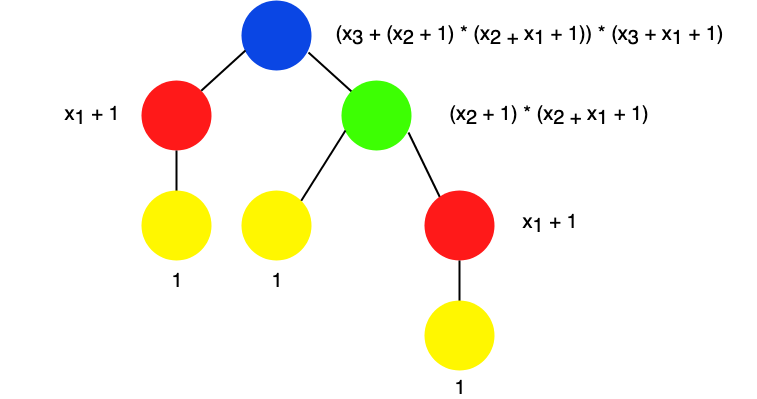
\includegraphics[width=8.5cm]{figuras/treeIsomorphism.png}
  \caption{Example of a tree with the hash of each node. }
\end{figure}


On the above picture we can see that the hash function is cumulative, and it forms a polynomial function in the end. The code for the above algorithm can be written as following in C++14:

\begin{lstlisting}
vector< vector<int> > adj; // Adjacency list of the graph
vector<long long> x; // X values for hash calculation
vector<int> d; // Height of each node
const int MOD = 1e9 + 7;
long long hashTree(int u, int p) {
   long long myHash = 1;
   for (int v : adj[u])
      if (v != p)
         myHash = (myHash * (d[h[u]] + hashTree(v, u))) % MOD;
   return myHash;
}
\end{lstlisting}

The hash of a tree can be defined recursively by the hashes of its subtrees. We can define the values of the array \( X \) as random values between \( 0 \) and \texttt{MOD - 1}. We can also trivially calculate the height of each node recursively. The algorithm described is linear.

One interesting caveat of this problem is that, although hashing trees to check for isomorphism only works with rooted trees, we can make it work for the problem of checking tree isomorphism for arbitrary trees. The basic idea is that we can root the tree by the center or centroid of tree (Because we know that we only have at most 2 centers or centroids on a tree). If we have more than one center or centroid, we can calculate the hash of the tree rooted by both and check if at least one of the hashed match. As this is not on the scope of this text I will limit the explanation here, but one can learn more about it in the bibliography \citep{Centroid}.

It is also important to cite here that there is another algorithm, the Aho-Hopcroft-Ulman algorithm, that runs in worst case linear time complexity that also solves the tree isomorphism problem. This algorithm is based on comparing both trees in a bottom up fashion \cite{AHU}.

SPOJ Problem: \url{https://www.spoj.com/problems/TREEISO}

%% May put there other applications such as consistent hashing 
\par

%% ------------------------------------------------------------------------- %%
\chapter{Final Remarks}
\label{cap:conclusions}

As we can see by previous chapters, hash functions and hash tables are very wide topics, with several details that we can have pages and pages with explanations. During this text the goal is to give a glance of how to implement a hash table data structure, with some other applications of the hash function itself.

It is important to notice that almost every programming language has it's implementation of a hash table, with some having a built-in implementation of a hash function for external usage. The most famous that we can cite here is Java, C++ (which have an implementation on STL), Golang, Python, Ruby, C\# and Scala. It's implementation may differ among paradigms as well, for example although in Scala Mutable hash maps uses chaining hashing, it also uses a Hash Trie for immutable hash maps, which is a complete different implementation with it's own specificalities and benefits for functional programming languages. \citep{hashMapAnalysis} 

One other interesting fact about hash tables is that it is an example about how memory locality is important in modern data structures. Memory locality is the proximity of the data accessed, which means that the data of your data structure is close to each other and it is ``cache friendly''. Although not accounted by usual complexity analysis, it is an important factor for regular used data structures, as one of the key performance factors of modern day processors.

During this text I also realized how deep we can go in each hash related topic. For that reason there are many contents that are not included here but are interesting to learn about. The main topics that would be included if I had more time were:

\begin{itemize}
\item Consistent Hashing
\item Distributed Hash Table
\item A deep analysis of the hash tables implemented during this text
\end{itemize}

Consistent hashing is a very interesting topic, because it is a special kind of hash function commonly used to implement sharded databases. It is special because when the table is resized, only \( \frac{K}{n} \) keys needs to be remapped on average, where K is the number of keys and N is the number of slots.\citep{wikiConsistent} This is very interesting and very useful in the context of databases because it easily allows horizontal scaling (that is, adding more machines).

Another interesting topic that I would have liked to discuss is distributed hash tables. A very used application in modern day, distributed hash table is a service that simulated a hash table lookup in a distributed environment. Common examples of this is modern services such as Memcached and Redis, that allow fast responses and scaling in modern web applications.

Lastly, it would be interesting to do a deep analysis of the hash tables implemented during this text. This would be different because we would see in practice many of the trade-offs discussed during this text, such as memory locality. There are many different factors in a deep analysis like this, like testing with different load factors, different deleting strategies, and different queries (random queries or queries closer to the 80/20 rule).

\par

\par


%%%%%%%%%%%%%%%%%%%%%%%%%%%% APÊNDICES E ANEXOS %%%%%%%%%%%%%%%%%%%%%%%%%%%%%%%%

% Um apêndice é algum conteúdo adicional de sua autoria que colabora com a
% ideia geral do texto mas que, por alguma razão, não precisa fazer parte
% da sequência do discurso; por exemplo, a demonstração de um teorema, as
% perguntas usadas em uma pesquisa qualitativa etc.
%
% Um anexo é um documento que não é de sua autoria mas que é relevante para
% a tese; por exemplo, a especificação do padrão que o trabalho discute.
%
% Os comandos appendix e annex reiniciam a numeração de capítulos e passam
% a numerá-los com letras. "annex" não faz parte de nenhuma classe padrão,
% ele foi criado para este modelo (em annex.sty e utils.tex). Se o
% trabalho não tiver apêndices ou anexos, remova estas linhas.
%
% Diferentemente de \mainmatter, \backmatter etc., \appendix e \annex não
% forçam o início de uma nova página. Em geral isso não é importante, pois
% o comando seguinte costuma ser "\chapter", mas pode causar problemas com
% a formatação dos cabeçalhos. Assim, vamos forçar uma nova página antes
% de cada um deles.

%%%% Apêndices %%%%
%\makeatletter
%\if@openright\cleardoublepage\else\clearpage\fi
%\makeatother

% Este formato está definido na package imeusp-headers.
%\pagestyle{appendix}

%\appendix

%\input{conteudo-exemplo/apendices}
%\input{conteudo/apendices}
%\par

%%%% Anexos %%%%
%\makeatletter
%\if@openright\cleardoublepage\else\clearpage\fi
%\makeatother

% Este formato está definido na package imeusp-headers (note que é o mesmo
% que o anterior; repetimos aqui caso você queira desabilitar toda a seção
% de apêndices).
%\pagestyle{appendix}

%\annex

%\input{conteudo-exemplo/anexos}
%\input{conteudo/anexos}
%\par


%%%%%%%%%%%%%%%%%%%%%%%%%%%%%% SEÇÕES FINAIS %%%%%%%%%%%%%%%%%%%%%%%%%%%%%%%%%%%

% Aqui vão a bibliografia, índice remissivo e outras seções similares.

% O comando backmatter desabilita a numeração de capítulos.
\backmatter

% Este formato está definido na package imeusp-headers
\pagestyle{backmatter}

% Espaço adicional no sumário antes das referências / índice remissivo
\addtocontents{toc}{\vspace{2\baselineskip plus .5\baselineskip minus .5\baselineskip}}

% A bibliografia é obrigatória

%%%%%%%%% Bibliografia com natbib (preterido): %%%%%%%%%
%\bibliographystyle{extras/alpha-ime}% citação bibliográfica alpha
%\bibliographystyle{extras/plainnat-ime} % citação bibliográfica textual
%\bibliography{bibliografia}  % associado ao arquivo: 'bibliografia.bib'

%%%%%%%% Bibliografia com biblatex (preferido): %%%%%%%%

\printbibliography[
  title=\refname\label{bibliografia}, % "Referências", recomendado pela ABNT
  %title=\bibname\label{bibliografia}, % "Bibliografia"
  % Inclui a bibliografia no sumário
  heading=bibintoc,
]

% imprime o índice remissivo no documento (opcional)
\printindex

\end{document}
